\documentclass[a4paper,twoside,DIV15,BCOR12mm]{scrbook}

\usepackage[utf8]{inputenc}
\usepackage{ngerman, url}
\usepackage{hyperref}
\usepackage{microtype}
\usepackage{tikz}
\usepackage{schnaubelt}
\usepackage{analysis}

\pdfinfo{
	/Author (Die Mitarbeiter von http://mitschriebwiki.nomeata.de/)
	/Title   (Funktionentheorie I)
	/Subject (Funktionentheorie I)
	/Keywords (Analysis)
}

\author{Prof. Dr. Roland Schnaubelt}
\publishers{Die Mitarbeiter von \url{http://mitschriebwiki.nomeata.de/}}
\title{Funktionentheorie I}
\date{Sommersemester 2009}
\makeindex

\begin{document}

\maketitle

\chapter*{Vorwort}

\section*{Über dieses Skriptum}
Dies ist ein Mitschrieb der Vorlesung \glqq Funktionentheorie I\grqq\
von Herrn Prof. Dr. Schnaubelt im Sommersemester 2009 an der Universität Karlsruhe (TH).
Die Mitschriebe der Vorlesung werden mit ausdrücklicher Genehmigung von Herrn Schnaubelt hier veröffentlicht,
Herr Schnaubelt ist für den Inhalt nicht verantwortlich.

\section*{Wer}
Beteiligt am Mitschrieb sind Michael Fütterer, Jonathan Zachhuber und
Alexander Koch.

\section*{Wo}
Alle Kapitel inklusive \LaTeX-Quellen können unter \url{http://mitschriebwiki.nomeata.de} abgerufen werden.
Dort ist ein \emph{Wiki} eingerichtet und von Joachim Breitner um die \LaTeX-Funktionen erweitert.
Das heißt, jeder kann Fehler nachbessern und sich an der Entwicklung
beteiligen. Auf Wunsch ist auch ein Zugang über \emph{Subversion} möglich.


\tableofcontents




\chapter{Komplexe Differenzierbarkeit}

\section{Vorbemerkungen zu \C}


%TODO Anfang

\begin{dfn} \label{dfn1.1}
  Eine Funktion $f\colon D \to \C$ heißt \emph{(komplex) differenzierbar} in $z_0 \in D$, wenn
  \[\lim_{z\to z_0}{\frac{f(z)-f(z_0)}{z-z_0}} \ad f^\prime(z_0)\]
  existiert. Dann heißt $f^\prime(z_0)$ die \emph{Ableitung} von $f$ bei $z_0$. Wenn $f$ bei allen $z_0\in D$ komplex
  differenzierbar ist, dann heißt $f$ \emph{holomorph}. Wir schreiben dann $f\in H(D)$. Iterativ definiert man höhere
  Ableitungen.
\end{dfn}

\begin{bem} \label{bem1.2}
\begin{enumerate}
\item Offenbar sind die Funktionen $f(x)=1$, $g(z)=z$ auf $\C$ holomorph mit $f^\prime(z)=0$, $g^\prime(z)=1$.
\item Genau wie in Analysis 1 zeigt man: Seien $f, g\colon D \to \C$ in $z\in D$ differenzierbar und $\alpha, \beta \in
  \C$. Dann sind auch $\alpha f + \beta g$, $f\cdot g$ und $\frac1f$ (wenn $f(z)\neq0$) in $z$ differenzierbar und es gelten die
  bekannten Regeln. Ebenso gilt die Kettenregel.
\item Polynome $p$ sind auf $\C$ und rationale Funktionen $f = \frac{p}{q}$ mit einem Polynom $q \neq 0$ sind auf $\{z\in\C:
  q(t) \neq 0\}$ holomorph mit den reellen Formeln für $p^\prime$, $f^\prime$.
\end{enumerate}
\end{bem}

\paragraph{Erinnerung an Analysis 1:} Gegeben seien $\kmplx{a_n}$ ($\nat{n}_0$) und ein $\kmplx{c}$. Die Potenzreihe
\[f(z) = \sum_{n=0}^\infty a_n(z-c)^n\]
konvergiert absolut für alle $z$ mit
\[|z-c| < \rho \da \left(\ls_{n\ra\infty}\sqrt[n]{|a_n|}\right)^{-1}\in[0,+\infty]\] 
und divergiert, falls $z\notin \bar{B}(c,\rho)$.

Reduktion auf $c=0$: Betrachte
\[h(w) \da f(c+w) = \sum_{n=0}^\infty a_n w^n,\]
wobei $w=z-c\in B(0,\rho)$, $z=c+w$.

\begin{satz}[vgl. Analysis 1, Theorem 4.12] \label{satz1.3} Sei
\[f(z) = \sum_{n=0}^\infty a_n(z-c)^n,\ z\in B(c,\rho),\]
eine Potenzreihe mit Konvergenzradius $\rho > 0$. Dann ist $f\in H(B(c,\rho))$ und
\[f^\prime(z) = \sum_{n=1}^\infty n a_n(z-c)^{n-1} =: g(z)\ (\forall z\in B(c,\rho)),\]
wobei die Potenzreihe $g$ den gleichen Konvergenzradius $\rho$ hat.

Sei $\nat{m}$. Iterativ folgt:
\[\exists f^{(m)}(z) = \sum_{n=m}^\infty n\cdot\dotsc\cdot (n-m+1) a_n(z-c)^{n-m}, \forall z\in B(c,\rho).\]
\end{satz}
\begin{proof} Wie in Analysis 1 zeigt man: $g$ hat Konvergenzradius $\rho$. Sei oBdA $c = 0$.

Seien $z\in B(0,\rho)$, $\ep>0$, $r>0$ mit $|z|<r<\rho$. Sei $w\in \bar{B}(0,r)$ mit $w\neq z$.

Da $\sum_{n=1}^\infty na_nr^{n-1}$ absolut konvergiert, existiert ein $N = \nat{N_\ep}$ mit
\begin{equation}\label{1.3s}0 \leq\!\!\! \sum_{n=N+1}^\infty\!\!\! n |a_n| r^{n-1} \leq \ep.\tag{$*$}\end{equation}

Ferner:
\[0\leq d(w) \da \biggl\lvert\frac{f(w)-f(z)}{w-z} - g(z)\biggr\rvert = \biggl\lvert\sum_{n=1}^\infty a_n\underbrace{\left(\frac{w^n-z^n}{w-z} - z^{n-1}\right)}_{\ad p_n(w)}\biggr\rvert\]
mit $p_n(w) = w^{n-1}+zw^{n-2}+\dotsb+z^{n-1}-nz^{n-1}$.
Dabei gelten:
\begin{itemize}
\item $p_n(w) \ra 0$, $w\ra z$ (für jedes feste $\nat{n}$)
\item \label{1.3ss}$|p_n(w)| \leq r^{n-1} + rr^{n-2} + \dotsb + r^{n-1} + nr^{n-1} = 2nr^{n-1}$ \hfill($\ast\ast$)
\end{itemize}

Damit folgt:
\begin{align*}
0&\leq d(w) \leq \sum_{n=1}^\infty |a_n||p_n(w)| \stackrel{\hyperref[1.3ss]{(**)}}{\leq} \sum_{n=1}^N |a_n||p_n(w)|\ + \sum_{n=N+1}^\infty 2n|a_n|r^{n-1}\\
&\stackrel{\eqref{1.3s}}{\leq} N \max\{|a_1||p_1(w)|,\dotsb,|a_n||p_n(w)|\} + 2\ep \ra 2\ep\ (w\ra z)\ (N = N_\ep\ \text{fest!})
\end{align*}

$\displaystyle\folgt \lim_{w\ra z} d(w) \leq 2\ep$. Da $\ep>0$ beliebig war, folgt $\displaystyle\lim_{w\ra z} d(w) = 0$.
\end{proof}

\paragraph{Beispiele} mit $\rho = \infty$.\begin{enumerate}
\item $\displaystyle \exp(z) \da \sum_{n=0}^\infty \frac{z^n}{n!},\ \exp^\prime(z) = \sum_{n=1}^\infty \frac{z^{n-1}}{(n-1)!} = \exp(z)$.
\item $\displaystyle \sin(z) = \sum_{n=0}^\infty \frac{(-1)^n}{(2n+1)!}z^{2n+1},\ \sin^\prime(z) = \sum_{n=0}^\infty \frac{(-1)^n}{(2n)!}z^{2n} = \cos(z).$
\item $\displaystyle \cos(z) = \sum_{n=0}^\infty \frac{(-1)^n}{(2n)!}z^{2n},\newline \cos^\prime(z) = \sum_{n=1}^\infty \frac{(-1)^n}{(2n-1)!}z^{2n-1} \stackrel{l=n-1}{=} \sum_{l=0}^\infty \frac{(-1)^{l+1}}{(2l+1)!}z^{2l+1} = -\sin(z).$
\end{enumerate}

%eine Trennlinie oder so?

\noindent Seien $f\colon D\ra\C$, $z_0\in D$, $z\in D$. Setze wieder $u = \Re f$, $v = \Im f$, $x_0 = \Re z_0$, $y_0 = \Im z_0$, also
\[f(x,y) = u(x,y) + \i v(x,y) = \cmplx{u(x,y)}{v(x,y)}.\]
Sei $z\neq z_0$ und $f$ bei $z_0$ komplex differenzierbar. Dann gilt:
\[\frac{1}{(z-z_0)}|f(z)-f(z_0)-f^\prime(z_0)(z-z_0)| = \left|\frac{f(z)-f(z_0)}{z-z_0} - f^\prime(z_0)\right| \ra 0,\ z\ra z_0.\]

Die Zahl $\kmplx{f^\prime(z_0)}$ kann als $\C$-lineare Abbildung $w\mapsto f^\prime(z_0)w$ aufgefasst werden. Diese ist dann auch $\R$-linear auf $\R^2$, kann also durch eine reelle $2\times 2$-Matrix dargestellt werden. Nach Analysis 2 ist nun $f$ in $z_0 = (x,y)$ reell differenzierbar und somit existieren die partiellen Ableitungen von $u$ und $v$ und es gilt:
\[\label{1.3+}f^\prime(x_0,y_0) = \left(\!\!\!\begin{array}{c c}\frac{\partial u}{\partial x} (x_0,y_0) & \frac{\partial u}{\partial y} (x_0,y_0)\\
\frac{\partial v}{\partial x} (x_0,y_0) & \frac{\partial v}{\partial y} (x_0,y_0)\end{array}\!\!\!\right).\tag{+}\]

\begin{satz} \label{satz1.4}
  Sei $f\colon D\ra\C$, $z_0 = x_0 + \i y_0\in D$. Dann sind äquivalent:
\begin{enumerate}
\item $f$ ist in $z_0$ komplex differenzierbar.
\item $f$ ist in $z_0$ reell differenzierbar und es gelten die \emph{Cauchy-Riemannschen Differentialgleichungen}
\begin{equation} \label{CR}
\frac{\partial u}{\partial x} (x_0,y_0) = \frac{\partial v}{\partial y} (x_0,y_0),\quad \frac{\partial u}{\partial y} (x_0,y_0) =
-\frac{\partial v}{\partial x} (x_0,y_0). \tag{CR}
\end{equation}
Insbesondere ist $f^\prime(z_0)$ schiefsymmetrisch.
\end{enumerate}
\end{satz}

\begin{proof} Die letzte Behauptung folgt aus \eqref{1.3+} und \eqref{CR}$_2$.

\noindent $(a) \folgt (b)$: Sei $r > 0$ mit $B(z_0,r) \subseteq D$, $\rat{t}$ mit $0 < |t| < r$. Dann gelten
\begin{align}
f^\prime(z_0) &= \lim_{t\ra 0} \frac{1}{t} (f(z_0+t) - f(z_0))\nonumber\\
&=  \lim_{t\ra 0} \left(\frac{1}{t} (u(x_0+t,y_0)-u(x_0,y_0)) + \frac{\i}{t} (v(x_0+t,y_0)-v(x_0,y_0))\right)\nonumber\\
&=\frac{\partial u}{\partial x} (x_0,y_0) + \i\frac{\partial v}{\partial x} (x_0,y_0)
\end{align} und \begin{align}
f^\prime(z_0) &= \lim_{t\ra 0} \underbrace{\frac{1}{\i t}}_{=-\frac{\i}{t}} (f(z_0+\i t) - f(z_0))\nonumber\\
&=  \lim_{t\ra 0} \left(-\i\frac{1}{t} (u(x_0,y_0+t)-u(x_0,y_0)) + \frac{\i}{\i t} (v(x_0,y_0+t)-v(x_0,y_0))\right)\nonumber\\
&=-\i\frac{\partial u}{\partial y} (x_0,y_0) + \frac{\partial v}{\partial y} (x_0,y_0).
\end{align}
Vergleichen von Real- und Imaginärteil liefert \eqref{CR}.

\noindent $(b) \folgt (a)$: Setze
\[w=\frac{\partial u}{\partial x} (x_0,y_0) + \i\frac{\partial v}{\partial x}\stackrel{\text{\eqref{CR}}}{=} \frac{\partial v}{\partial y} (x_0,y_0) - \i\frac{\partial u}{\partial y}(x_0,y_0) \in\C.\]
Dann gilt:
\[w(z-z_0) = (\Re w)(x-x_0) - (\Im w)(y-y_0) + \i((\Re w)(y-y_0) + (\Im w)(x-x_0))\]
\[\stackrel{\text{Def. $w$}}{=} \cmplx{\frac{\partial u}{\partial x} (x_0,y_0)(x-x_0) + \frac{\partial u}{\partial y}(x_0,y_0)(y-y_0)}{\frac{\partial v}{\partial y} (x_0,y_0)(y-y_0) + \frac{\partial v}{\partial x}(x_0,y_0)(x-x_0)}\ \text{(in $\R^2$)}.\]
\begin{align*}
\displaystyle\folgt &|f(z)-f(z_0)-w(z-z_0)|\frac{1}{|z-z_0|}\\
&\qquad= \left|\cmplx{x-x_0}{y-y_0}\right|_2^{-1} \left|\cmplx{u(x,y)-u(x_0,y_0)-\left(\nabla u(x_0,y_0)\mid\cmplx{x-x_0}{y-y_0}\right)}{v(x,y)-v(x_0,y_0)-\left(\nabla v(x_0,y_0)\mid\cmplx{x-x_0}{y-y_0}\right)}\right|_2 \ra 0,
\end{align*}

%$\displaystyle\underbrace{(x,y)}_{=z} \ra \underbrace{(x_0,y_0)}_{=z_0}$,
für $(x_0,y_0)=z_0 \to z=(x,y)$,
da $u$, $v$ differenzierbar.
\end{proof}

\begin{bsp} \label{bsp1.5}
\begin{enumerate}
\item $f(z) = \bar{z}$, $\kmplx{z}$, ist nirgends komplex differenzierbar, obwohl $f(x,y) = \cmplx{x}{-y}$ reell $C^\infty$ ist. Denn $u(x,y) = x$, $v(x,y) = -y$; also 
\[\frac{\partial u}{\partial x}(x,y) = 1 \neq -1 = \frac{\partial v}{\partial y}(x,y),\]
was \eqref{CR}$_1$ widerspricht.
\item $f(z) = |z|^2 = x^2 + y^2$, $\kmplx{z}$, ist nur in $z=0$ komplex differenzierbar, denn hier ist $u(x,y) = x^2+y^2$, $v(x,y) = 0$ und somit:
\[\frac{\partial u}{\partial x}(x,y) = 2x \stackrel{!}{=} \frac{\partial v}{\partial y}(x,y) = 0 \gdw x=0,\]
\[\frac{\partial u}{\partial y}(x,y) = 2y \stackrel{!}{=} -\frac{\partial v}{\partial x}(x,y) = 0 \gdw y=0.\]
\item $\displaystyle f(z) = \frac{1}{z} = \frac{\bar{z}}{|z|^2} = \underbrace{\frac{x}{x^2+y^2}}_{=u} + \i\underbrace{\frac{-y}{x^2+y^2}}_{=v}$ ist holomorph für $z\neq 0$ (Bem.~\ref{bem1.2}).
\end{enumerate}
\end{bsp}

\begin{bem} \label{bem1.6}
Sei $f$ in $z = x+\i y$ komplex differenzierbar. Nach (+) und \eqref{CR} gilt:
\begin{equation}
A \da f^\prime(z) = \left(\!\!\!\begin{array}{c c}\frac{\partial u}{\partial x}(x,y)&\frac{\partial u}{\partial y}(x,y)\\-\frac{\partial u}{\partial x}(x,y)&\frac{\partial u}{\partial x}(x,y)\end{array}\!\!\!\right) = \left(\!\!\!\begin{array}{c c}\frac{\partial v}{\partial y}(x,y)&-\frac{\partial v}{\partial x}(x,y)\\\frac{\partial v}{\partial x}(x,y)&\frac{\partial v}{\partial y}(x,y)\end{array}\!\!\!\right).
\end{equation}
Also gilt $\rho \da \displaystyle \det A = \frac{\partial u}{\partial x}(x,y)^2 + \frac{\partial u}{\partial y}(x,y)^2 =
\frac{\partial v}{\partial x}(x,y)^2 + \frac{\partial v}{\partial y}(x,y)^2 \geq 0$ und \\ $f^\prime(z) \neq 0 \gdw \det A > 0$.
Ferner ist $A^TA = (\det A)\I$. Sei $f^\prime(z) \neq 0$. Dann gilt
\[\label{1.6s}\frac{1}{\sqrt{\rho}}A \text{ orthogonal} \tag{$*$}\]
\[\label{1.6ss}\folgt \abs{Av}_2 = \sqrt{\rho} \abs{v}_2 \quad (\forall v \in \R^2). \tag{$**$}\]
Sei $\gamma_j \in C^1((-1,1), \R^2)$ eine Kurve in $D$ mit $\gamma_j(0) = (x, y)$, $\gamma_j^\prime(0) \ad v_j \in \R^2
\setminus \{(0,0)\}$ ($j=1,2$). Dann ist $Av_j = (f \circ \gamma_j)^\prime(0) = f^\prime(x, y) \gamma_j^\prime(0)$ ein
Tangentenvektor der Bildkurve $f \circ \gamma_j$ bei $f(x, y)$ ($j=1,2$). Weiter gilt: \[\frac{(v_1\mid v_2)}{\abs{v_1}_2
  \abs{v_2}_2} \nach{=}{\eqref{1.6s},\eqref{1.6ss}} \frac{\frac1\rho (Av_1\mid Av_2)}{\frac1\rho \abs{Av_1}_2 \abs{Av_2}_2},\]
woraus durch Anwenden des Arcuscosinus folgt: $\sphericalangle(v_1,v_2) = \sphericalangle(Av_1,Av_2)$ (Winkel ohne Orientierung).\\
Also ist der Winkel der Urbildtangenten gleich dem Winkel der Bildtangenten unter $f$. Falls also $f^\prime(z)\neq0$, dann ist
$f$ bei $z=x+\i y$ \emph{winkeltreu} (``konform''). Ferner ist $f$ orientierungstreu, da $\det A > 0$.
\end{bem}
%TODO Bild!

\begin{dfn} \label{dfn1.7}
Seien $U, V \subseteq \C$ offen und nichtleer. Sei $f\colon U \to V$ bijektiv und $f\in H(U)$, $f^{-1}\in H(V)$. Dann heißt $f$ \emph{biholomorph}. (Dann heißen $U$ und $V$ auch ``konform äquivalent''.)
\end{dfn}

\begin{satz} \label{satz1.8}
\begin{enumerate}
\item\label{satz1.8a} Seien $U, V \subseteq \C$ offen und nichtleer, $f\colon U \to V$ biholomorph. Dann ist $f^\prime(z)\neq 0$ für alle $z\in U$ und es gilt
\[(f^{-1})^\prime(f(z)) = (f^{-1})^\prime(w) = \frac{1}{f^\prime(f^{-1}(w))} = \frac{1}{f^\prime(z)} \quad (\forall z\in U,\ \forall w=f(z) \in V)\]
\item Seien $f\in H(D) \cap C^1(D, \R^2)$, $z_0\in D$, $f^\prime(z_0)\neq0$. Dann exisieren offene $U, V \subseteq \C$ mit $z_0\in U$, $f(z_0)\in V$, sodass $f\colon U \to V$ biholomorph ist. Somit ist a) auf $f$ für alle $z\in U$ und $w=f(z)\in V$ anwendbar.
\end{enumerate}
\end{satz}
\begin{proof}
\begin{enumerate}
\item Nach Bem.~\ref{bem1.2} und $z=f^{-1}(f(z))$ ($\forall z\in U$) folgt $1 = (f^{-1})^\prime(f(z))f^\prime(z)$. Durchdividieren ergibt Behauptung a).
\item Nach Bem.~\ref{bem1.6} ist $f^\prime(z_0)$ als $2\times2$-Matrix invertierbar. Der Umkehrsatz aus Analysis 2 liefert Behauptung b).\qedhere
\end{enumerate}
\end{proof}

\begin{dfn*} Eine Funktion $u\in C^2(D, \R)$ heißt \emph{harmonisch} auf $D$, wenn für alle $(x, y) \in D$ gilt:
\[\triangle u(x, y) \da \frac{\partial^2u}{\partial x^2}(x, y) + \frac{\partial^2u}{\partial y^2}(x, y) = 0.\]
\end{dfn*}

\begin{satz} \label{satz1.9}
\begin{enumerate}
\item Sei $f\in H(D) \cap C^2(D, \R^2)$. Dann sind $u=\Re f$, $v = \Im f$ harmonisch auf $D$.
\item Sei $u \in C^2(D, \R)$ auf $D$ harmonisch, $B_0 \da B((x_0,y_0),r) \subseteq D$ für ein $r>0$, $(x_0,y_0)\in D$. Dann existiert ein $f\in H(B_0)$ mit $u = \Re f$.
\end{enumerate}
\end{satz}
\begin{proof}
\begin{enumerate}
\item Der Satz von Schwarz aus Analysis 2 (Satz 2.21) liefert
\[\frac{\partial^2u}{\partial x^2} + \frac{\partial^2u}{\partial y^2} \nach{=}{\eqref{CR}}
\frac{\partial}{\partial x} \frac{\partial v}{\partial y} - \frac{\partial}{\partial y} \frac{\partial v}{\partial x} = 0.\]
\item Setze für $(x, y) \in B_0$
\[v(x, y) = - \Integral{x_0}{x}{\frac{\partial u}{\partial y}(s, y_0)}{s} +
\Integral{y_0}{y}{\frac{\partial u}{\partial x}(x, s)}{s}.\]
Beachte: die Strecken von $(x_0,y_0)$ nach $(x,y_0)$ und von $(x,y_0)$ nach $(x,y)$ liegen in $B_0$. Analysis 1 und 2 liefern: $v\in C^1(B_0)$ und
\begin{multline*}
\frac{\partial v}{\partial x}(x, y) = - \frac{\partial u}{\partial y}(x, y_0) + \Integral{y_0}{y}{\underbrace{\frac{\partial^2 u}{\partial x^2}(x, s)}_{\nach{=}{n.V.} - \frac{\partial^2 u}{\partial y^2}(x,s)}}{s}\\
= - \frac{\partial u}{\partial y}(x, y_0) - \frac{\partial u}{\partial y}(x, y) + \frac{\partial u}{\partial y}(x, y_0)
= - \frac{\partial u}{\partial y}(x, y)
\end{multline*}
\folgt \eqref{CR}$_2$.
Ferner $\frac{\partial v}{\partial y}(x, y) = \frac{\partial u}{\partial x}(x, y)$ \folgt \eqref{CR} gilt. Mit
Satz~\ref{satz1.4} folgt: $f=u+\i v$ ist auf $B_0$ holomorph. \qedhere
\end{enumerate}
\end{proof}

\begin{bsp*}
Sei $f(z) = z^3 = (x+\i y)^3 = x^3 + 3\i x^2 y - 3xy^2 - \i y^3$. Satz~\ref{satz1.9} liefert: $u(x,y) = \Re f(x, y) = x^3 - 3xy^2$ ist harmonisch auf $\C$.
\end{bsp*}


\section{Elementare Funktionen}

\subsection{Möbiustransformationen}

\noindent Sei $A = \mat{a}{b}{c}{d} \in \mathrm{M}_{22}(\C)$ mit $\det A = ad-bc \neq 0$ (dann ist $c\neq0$ oder
$d\neq0$). Setze
\[m_A(z) = \frac{az+b}{cz+d} \quad \  \text{für} \quad z \in D_A \da
\begin{cases} \C \setminus \left\{-\frac{d}{c}\right\} ,& c \neq 0, \\ \C ,& c = 0. \end{cases}\]
$m_A$ heißt \emph{Möbius-Transformation}. Offensichtlich ist $m_A \in H(D_A)$.
\paragraph{Eigenschaften.} Sei $A$ wie oben und $\tilde{A} = \mat{\tilde{a}}{\tilde{b}}{\tilde{c}}{\tilde{d}} \in
\mathrm{M}_{22}(\C)$ mit $\det \tilde{A} \neq 0$.
\begin{enumerate}
\item Es gilt
  \[m_A(z) = z \; (\forall z \in D_A) \gdw A = \mat{a}{0}{0}{a} \text { für ein } a \in \C \setminus \{0\}.\]
  \begin{proof}
    "`$\Leftarrow$"': einsetzen! "`$\Rightarrow$"': Für alle $z\in D$ gilt:
    \[m_A(z)=z \folgt cz^2 + (d-a)z - b = 0 \text{ (}\forall z\in D_A\text{) }\]
    \[\folgt c=0, d=a, b=0 \folgt A = \mat{a}{0}{0}{a}. \qedhere\]
  \end{proof}
\item Für alle $\alpha\in\C$ gilt $m_{\alpha A} = m_A$.
\item Es gilt $m_A(m_{\tilde{A}}(z)) = m_{A\tilde{A}}(z)$ (soweit alles definiert).
\begin{proof} Für passende $z$:
  \[m_A(m_{\tilde{A}}(z)) =
  \frac{a\frac{\tilde{a}z+\tilde{b}}{\tilde{c}z+\tilde{d}}+b}{c\frac{\tilde{a}z+\tilde{b}}{\tilde{c}z+\tilde{d}}+d} =
  \frac{(a\tilde{a}+b\tilde{c})z+(a\tilde{b}+b\tilde{d})}{(c\tilde{a}+d\tilde{c})z+(c\tilde{b}+d\tilde{d})} =
  m_{A\tilde{A}}(z). \qedhere\]
\end{proof}
\item Es gilt: $\displaystyle A^{-1} = \frac{1}{ad-bc}\mat{d}{-b}{-c}{a}$. Damit folgt: $\displaystyle D_{A^{-1}}=
  \begin{cases} \C\setminus\left\{\frac{a}{c}\right\},&c\neq 0,\\\C,&c=0.\end{cases}$

Man zeigt leicht, dass gilt:
\[\label{m:s}m_A(D_A) \subseteq D_{A^{-1}},\tag{$\ast$}\]
\[\label{m:ss}m_{A^{-1}}(D_{A^{-1}}) \subseteq D_A.\tag{$\ast\ast$}\]
Also folgt aus c): $m_A(D_A) = D_{A^{-1}}$ (wende auf \eqref{m:ss} $m_A$ an), $m_{A^{-1}}(D_{A^{-1}}) = D_A$ (wende auf \eqref{m:s} $m_{A^{-1}}$ an) und $(m_A)^{-1} = m_{A^{-1}}$.

Insbesondere sind $m_A\colon D_A\ra D_{A^{-1}}$, $m_{A^{-1}}\colon D_{A^{-1}}\ra D_A$ biholomorph.
\item\label{eigenschaften:e} Sei $c=0$ (also $d\neq0$). Dann ist $m_A(z) = \frac{a}{d}z + \frac{b}{d}$ eine affine Abbildung, also $m_A = T \circ S$
  mit $Tw=w+\frac{d}{d}$ (Translation) und $Sw = \frac{a}{d}w$ (Drehstreckung). Sei nun $c\neq0$. Dann gilt $m_A = A_2 \circ J
  \circ A_1$, wobei $A_1w = cw+d$, $A_2w = \frac{a}{c} - \frac{ad-bc}{c}w$ (affin) und $Jw = \frac1w$ ($w\neq0$) (Inversion).
  \begin{proof}
    Es gilt $\displaystyle\frac{az+b}{cz+d} = \frac{a}{c} - \frac{ad-bc}{c}\frac{1}{cz+d} = A_2(J(A_1(z)))$.
  \end{proof}
%%%%%%%%%%%%%%%%%%%%%%%%%%%%
% Eigentlich aus der nächsten Vorlesung, muss aber glaub
% ich hier hin ....
%%%%%%%%%%%%%%%%%%%%%%%%%%%%
Fasse jede Gerade in $\C$ als verallgemeinerten Kreis über $\infty$ auf. Also ist ein verallgemeinerter Kreis $K$ entweder eine Gerade oder eine echte Kreislinie. Beachte: $K$ wird durch die Angabe dreier verschiedener Punkte in $\C_\infty$ eindeutig bestimmt.
\item\label{eigenschaften:f} Jede Möbiustransformation bildet einen verallgemeinerten Kreis bijektiv auf einen verallgemeinerten Kreis ab.
\begin{proof} Nach \ref{eigenschaften:e}
%%%%%%%%%%%%%%%%%%%%%%%
% Da steht im Moment eine 5, obwohl da ein e sein sollte ...
% das Problem hatten wir glaub ich schonmal, weiß aber nicht
% mehr die Lösung ;-)
%%%%%%%%%%%%%%%%%%%%%%%
 ist die Behauptung nur für Translationen $T$, Drehstreckungen $S$ und die Inversion $J$ zu zeigen. Klar: $T$, $S$ sind ``verallgemeinert kreistreu.''

Zu $J$: Sei $r>0$, $\kmplx{z_0}$. Dann:
\[z\in K\da \partial B(z_0,r)\gdw r^2 = |z-z_0|^2 = (z-z_0)(\bar{z}-\bar{z_0}) = |z|^2-z_0\bar{z}-\bar{z_0}z+|z_0|^2.\]
Damit: 
\[\label{m:f:s}K=\{\kmplx{z}: \alpha|z|^2+c\bar{z}+\bar{c}z+\delta = 0\}\tag{$*$}\]
für feste $\alpha$, $\delta\in\R$, $\kmplx{c}$ mit $|c|^2>\alpha\delta$, wobei $z_0=-\frac{c}{\alpha}$, $r^2=\frac{|c|^2}{\alpha^2}-\frac{\delta}{\alpha}$, falls $\alpha\neq 0$.

$\leadsto$ Für $\alpha\neq 0$ beschreibt \eqref{m:f:s} die echte Kreislinie $\partial B(z_0,r)$. Für $\alpha = 0$ beschreibt \eqref{m:f:s} die Gerade $\Re(\bar{c}z) = -\frac{\delta}{2}$ (Beachte: $c\neq 0$). Multipliziere \eqref{m:f:s} mit $\frac{1}{|z|^2}$. Dann erfüllt $w = Jz = \frac{1}{z} = \frac{\bar{z}}{|z|^2}$ die Gleichung:
\[ 0 = \underbrace{\alpha}_{\ad\delta'} + \underbrace{cw}_{\ad -\bar{c}'} + \underbrace{\bar{c}\bar{w}}_{\ad -c'} + \underbrace{\delta|w|^2}_{\ad\alpha'}.\]
Weiter gilt: $|c'|^2-\alpha'\delta' = |c|^2-\alpha\delta > 0$. Wenn $K$ durch \eqref{m:f:s} beschrieben wird, dann folgt also $J(K)\subseteq K'$, wobei $K'$ ein verallgemeinerter Kreis ist. Genauso: $J(K')\subseteq K$. Da $J^2 = \id$ folgt $K'=J^2(K')\subseteq J(K)\folgt J(K)=K'$.
\end{proof}
\end{enumerate}

%%%%%%%%%%%%%%%%%%%%%%%
% Aus der vorherigen Vorlesung, gehört aber glaub
% ich dahinter .....
%%%%%%%%%%%%%%%%%%%%%%%
\begin{dfn} \label{dfn1.10}
  Setze $\C_\infty = \C \cup \{\infty\}$, $\R_\infty = \R \cup \{\infty\}$, wobei gelten soll:
\begin{eqnarray*}
&\forall\kmplx{z}: z+\infty = \infty + z = \infty,\ \frac{z}{\infty} = 0,\\
&\forall\kmplx{z}\setminus \{0\}: z\cdot\infty = \infty\cdot z = \infty,\ \frac{z}{0} = \infty.
\end{eqnarray*}
\textbf{Verboten:} $0\cdot\infty$, $\infty\cdot 0$, $\frac{0}{0}$, $\frac{\infty}{\infty}$.

\noindent Wir schreiben $z_n \ra \infty$, wenn $\abs{z_n} \ra +\infty\ (n\ra\infty)$.

\noindent Beachte: Dieses $\infty$ ist ein anderes als $\pm\infty$ in $\R$ aus Analysis 1.
\end{dfn}

Setze bezüglich dieser ``Konvergenz'' $m_A$ ``stetig'' fort durch
\[m_A (\infty) \da \left\{\!\!\!\begin{array}{r @{,\ } l}\frac{a}{c}&c\neq 0\\\infty&c=0\end{array}\right..\]
Beachte:
\[m_A(z)=\frac{a+\frac{b}{z}}{c+\frac{d}{z}}\ (z\neq 0),\ m_A\left(-\frac{d}{c}\right) = \infty\]
(beachte: $-\frac{ad}{c} + b\neq 0$, da $\det A\neq 0$).

Mit etwas Rechnung folgt: $m_A\colon\C_\infty\ra\C_\infty$ ist bijektiv mit $(m_A)^{-1} = m_{A^{-1}}\colon\C_\infty\ra\C_\infty$.

Sei $\mathcal{M}\da\{m_A\colon\C_\infty\ra\C_\infty\mid\det A\neq 0\}$. Mit obigen Eigenschaften (und etwas Rechnung bezüglich $\infty$) folgt:
\begin{itemize}
\item $\mathcal{M}$ ist eine Gruppe bezüglich der Komposition.
\item $\Phi\colon \mathrm{GL}(2,\C)\ra\mathcal{M}$, $A\mapsto m_A$ ist ein surjektiver Gruppenhomomorphismus mit
  $\mathrm{Kern }\Phi = \{\alpha \I \mid \kmplx{\alpha}\setminus\{0\}\}.$
\end{itemize}
%%%%%%%%%%%%%%%%%%%%%%%%%%%%%

\begin{bsp}[Cayley-Transformation]
Sei $C=\mat{1}{-\i}{1}{\i}$ ($\leadsto\det C = 2\i\neq 0$) $\displaystyle\leadsto M_C(z) = \frac{z-\i}{z+\i}$.

Dabei: $\displaystyle M_C(-\i) = \frac{-2}{0} = \infty$, $\displaystyle M_C(\infty) = \frac{1-\frac{\i}{\infty}}{1+\frac{\i}{\infty}} = 1$. Weiter: $\displaystyle M_C(0) = -1$, $\displaystyle M_C(1) = \frac{1-\i}{1+\i} = -\i$. Durch $\{0,1,\infty\}$ läuft der verallgemeinerte Kreis $\R_\infty = \R\cup\{\infty\}$. Nach \label{eigenschaften:f} %%s.o.
verläuft der Bildkreis $M_C(\R_\infty)$ durch die Bilder $-1,-\i,1$. Dies ist $\set{S} = \partial \set{D}$ mit $\set{D} = B(0,1)$. Also $M_C(\R_\infty) = \set{S}$.

Ferner: Für $b\in\R\setminus\{-1\}$ gilt $\displaystyle M_C(\i b) = \frac{b-1}{b+1}$, insbesondere $M_C(\i) = 0$. $\i\R_\infty$ verläuft durch $0,\i,\infty$. $\R_\infty$ verläuft durch die Bildpunkte $-1,0,1 \folgt M_C(\i\R_\infty) = \R_\infty$. Mit Analysis 1: $M_C(\i\R_+) = [-1,1)$.

%% Bild
\begin{tikzpicture}[scale=2]

\draw[->] (0,-1.5) -- (0,1.5);
\draw[->] (-1.5,0) -- (1.5,0);
\filldraw [gray] (0,0) circle (1pt);
\draw (0,0) node [anchor=north west] {$0$};
\filldraw [gray] (1pt,0.95) -- (0,1.07) -- (-1pt,0.95) -- cycle;
\draw (-1pt,1) -- (1pt,1);
\draw (0,1) node [anchor=west] {$\i$};
\draw [blue] (-1.5,0.6) -- (1.5,0.6);
\filldraw [blue] (0,0.6) circle (1pt);
\draw [blue] (0,0.73) arc (90:180:1.3mm);
\draw [blue] (-0.5mm,0.65) node {.};
\draw (1,1pt) -- (1,-1pt);
\draw (0.97,1pt) -- (1.03,-1pt);
\draw (0.97,-1pt) -- (1.03,1pt);
\draw (1,0) node [anchor=north] {$1$};
\draw [gray] (-1.8,0) node [shape=rectangle,fill] {};
\draw (-1.8,0) node [anchor=north] {$\infty$};
\draw [red] (-1.8,0) -- (1.5,0);
\draw [green] (0,-1.5) -- (0,1.5);

\begin{scope}[xshift=4cm]
\draw[->] (0,-1.5) -- (0,1.5);
\draw[->] (-1.5,0) -- (1.5,0);
\draw[red] (0,0) circle (1cm);
\filldraw[gray] (-1,0) circle (1pt);
\draw (-1,0) node [anchor=north] {$-1$};
\draw (-1pt,-1) -- (1pt,-1);
\draw (-1pt,-0.97) -- (1pt,-1.03);
\draw (-1pt,-1.03) -- (1pt,-0.97);
\draw (0,-1) node [anchor=east] {$-\i$};
\filldraw [gray] (1pt,-1pt) -- (-1pt,-1pt) -- (0,1pt) -- cycle;
\draw (0,0) node [anchor=north west] {$0$};
\draw [gray] (1,0) node [shape=rectangle,fill] {};
\draw (1,0) node [anchor=north] {$1$};
\filldraw [blue] (-0.6,0) circle (1pt);
\draw [blue] (0.2,0) circle (0.8);
\draw [blue] (-0.6,0) -- (-0.6,0.13) arc (90:180:1.3mm);
\draw [blue] (-0.65,0.5mm) node {.};
\draw [blue] (-1,-1) node[anchor=north] {$M_C(\i b)$};
\draw [blue,->] (-1,-1) -- (-0.65,-0.05);
\draw [green] (-1.5,0) -- (1.5,0);
\end{scope}

\draw[->] (1.5,0.8) .. controls (1.8,1.2) and (2.2,1.2) .. (2.5,0.8);
\draw (2,1.3) node {$M_C$};

\end{tikzpicture}

Die Gerade $K\colon \i b + x$, $\reell{x}$, ($b>0$ fest) wird auf den verallgemeinerten Kreis $K'$ durch $M_C(\i b)\in (-1,1)$ und $1 = M_C(\infty)$ abgebildet. Nach Bem. \ref{bem1.6} und da $K'$ die imaginäre Achse im Winkel $\frac{\pi}{2}$ schneidet, schneidet $M_C(K)$ die reelle Achse ($=M_C(\i\R_\infty)$) auch senkrecht in $M_C(\i b)$. $\folgt M_C(K)$ ist symmetrisch zur $x$-Achse und liegt in $\set{D}\folgt M_C(\set{H}_+)\subseteq\set{D}$, mit $\set{H}_+ = \{\kmplx{z}:\Im{z}>0\}$. Sei weiter $w\in\set{D}$. Sei $K$ der Kreis durch $w$ und $1$, der symmetrisch zur $x$-Achse ist. Sei $a\in (-1,1)$ der zweite Schnittpunkt von $K$ mit der $x$-Achse $\folgt$ Es gibt genau ein $b\in (0,+\infty)$ mit $\displaystyle a = \frac{b-1}{b+1}$. Also: Ist $w\in M_C(\i b + \R_\infty)\folgt M_C(\set{H}_+) = \set{D}\folgt M_C\colon\set{H}_+\ra\set{D}$ ist biholomorph.
\end{bsp}

\subsection{Potenzen und Wurzeln}

Sei $\nat{n}$, $n\geq 2$. Mit $\sqrt[n]{x}$ wird stets die reelle Wurzel bezeichnet. Für $\theta\in (0,\pi]$ definiere den (offenen) Sektor:
\[\Sigma_\theta \da \{z\in\C\setminus\{0\}: |\arg z| < \theta\}\]
speziell: $\Sigma_\pi = \C\setminus\R_-$ (geschlitzte Ebene), $\Sigma_\frac{\pi}{2} = \{\kmplx{z}: \Re{z} > 0\} = \C_+$ (rechte Halbebene)

\mbox{
\begin{minipage}[c]{.5\textwidth}
\begin{center}
\begin{tikzpicture}[scale=1.5]
\draw [->] (0,-1) -- (0,1);
\draw [->] (-1,0) -- (1,0);
\draw (0,0) -- (50:1.2);
\draw (0,0) -- (-50:1.2);
\draw (50:0.6) arc (50:-50:0.6);
\draw (30:1) node [anchor=west] {$\Sigma_\theta$, $\theta < \frac{\pi}{2}$};
\end{tikzpicture}
\end{center}
\end{minipage}
\begin{minipage}[c]{.5\textwidth}
$z = r\e^{\i\phi}\in\Sigma_\theta \gdw r > 0,\ |\phi| < \theta$

(wobei $|\phi| \leq \pi$)
\end{minipage}
}

Betrachte: $P_n(z) = z^n$, $\kmplx{z}$. Dann: $P_n(r\e^{\i\phi})=r^n\e^{\i\phi n}$. Also bildet $P_n$ den Halbstrahl $\{r\e^{\i\phi},\ r>0\}$ mit Winkel $\phi\in(-\pi,\pi]$ bijektiv auf den Halbstrahl $\{s\e^{\i\phi n},\ s>0\}$ mit $n$-fachem Winkel (modulo $2\pi$) ab.

Setze $p_n\da {P_n}|_{\Sigma_\frac{\pi}{n}}$. Dann ist $p_n\colon\Sigma_\frac{\pi}{n} \ra \Sigma_\pi$ bijektiv.

Beachte: $P_n$ ist schon auf $\bar{\Sigma_\frac{\pi}{n}}$ nicht mehr injektiv. Beispiel für $n=2$:
\[+\i,-\i\in\bar{\Sigma_\frac{\pi}{2}} = \bar{\C_+},\ P_2(\i) = -1 = P_2 (-\i).\]

\begin{dfn}\label{dfn1.12} Der Hauptzweig der $n$-ten Wurzel ist die Umkehrabbildung $r_n = p_n^{-1}\colon \Sigma_\pi\ra \Sigma_\frac{\pi}{n}$. Man schreibt $r_n(w) \ad w^\frac{1}{n}$ für $w\in\Sigma_\pi$.
\end{dfn}

%% Strich?

Per Definition haben wir $r_n(z^n) = z\ (\forall z\in\Sigma_\frac{\pi}{n})$, $r_n(w)^n = w\ (\forall w\in\Sigma_\pi)$. Es gilt:
\begin{equation}\label{1.5}
r(s\e^{\i\psi}) = \sqrt[n]{s}\e^{\i\frac{\psi}{n}}\ (\forall s > 0,\ |\psi| < \pi)
\end{equation}
(denn: $z=\sqrt[n]{s}\e^{\i\frac{\psi}{n}}\in\Sigma_\frac{\pi}{n}$ und $z^n = s\e^{\i\psi}$)

Insbesondere: $r_n(x) = \sqrt[n]{x}$ für $x>0$.

Weiter: ${p_n}^\prime(z) = nz^{n-1}\neq 0\ (\forall z\in\Sigma_\frac{\pi}{n})$.

Mit Satz \ref{satz1.8} sind $r_n\in H(\Sigma_\pi)$ und
\[\left.\begin{array}{r l}p_n\colon&\Sigma_\frac{\pi}{n}\ra\Sigma_\pi\\r_n\colon&\Sigma_\pi\ra\Sigma_\frac{\pi}{n}\end{array}\right\}\text{biholomorph}\]

\subsubsection*{Abbildungsverhalten der Quadratfunktion}
\begin{itemize}
\item {\bf Vertikale Gerade} $\Re z = a$ mit einem festen $a>0$. Also gilt für $z=x+\i y$, dass $w \da z^2=a^2-y^2 + \i\cdot2ay$
  (mit $a=x$) (\reell{y} ist Parameter). Also ist $\Im w = 2ay$, also $y = \frac{\Im w}{2a}$. Damit folgt:
  \[\Re w = a^2-y^2 = a^2 - \frac{(\Im w)^2}{4a^2} \le a^2.\]
  Also ist $\Im w = \pm 2a\sqrt{a^2-\Re w}$ eine nach links offene Parabel mit Scheitel $(a^2,0)$.
\item {\bf Horizontale Gerade} $\Im z = b$ mit einem festen $b>0$. Also gilt für $z=x+\i y$, dass $w \da z^2 = x^2-b^2 + \i\cdot
  2bx$ (mit $y=b$) (\reell{x} ist Parameter). Wie oben erhält man $\Im w = 2bx$, also $x=\frac{\Im w}{2b}$ und $\Re w =
  x^2-b^2$. Also ist $\Im w = \pm 2b\sqrt{b^2+\Re w}$ eine nach rechts offene Parabel mit Scheitel $(-b^2,0)$.
\end{itemize}

%%%%%%%%%%%%%%%%%%%%%%%%%
\begin{center}
\begin{tikzpicture}[scale=3]

\draw[->] (-0.5,0) -- (1.2,0);
\draw[->] (0,-0.5) -- (0,1.2);

\draw[blue] (-0.5,0.5) -- (1.2,0.5);
\draw[blue] (-0.02,0.52) -- (0.02,0.48);
\draw[blue] (-0.02,0.48) -- (0.02,0.52);
\draw[blue] (0,0.5) node [anchor=north west] {$\i b$};

\filldraw[red] (30:1) -- +(0,0.5) -- ++(0,-0.5) circle (0.5pt) -- +(0,0) node [above right] {$a$} -- +(0,-0.5);

\draw (0,0) -- (30:1);
\filldraw (30:1) circle (0.5pt);
\draw (30:1) node [below right] {$z$};
\draw (0.2,0) arc (0:30:0.2);
\draw (22:0.2) node [anchor=west] {$\phi$};

\draw (1,1pt) -- (1,-1pt);
\draw (1,0) node [below] {1};
\draw (-1pt,1) -- (1pt,1);
\draw (0,1) node [right] {$\i$};
\draw (-0.3,0.7) node {Urbild};

\begin{scope}[xshift=2.5cm]
\draw[->] (-0.5,0) -- (1.2,0);
\draw[->] (0,-1.7) -- (0,1.7);

\filldraw[red] (0.75,0) circle (0.5pt);
\draw[red] (0.75,0) node [above right] {$a^2$};
%\filldraw (0,1.5) circle (0.5pt);

\begin{scope}[red,xshift=0.75cm,rotate=90]
% 1/3 x^2
\draw (0,0) parabola (1.65,0.9075);
\draw (0,0) parabola (-1.65,0.9075);
\end{scope}

\draw[blue] (-0.25,0) node [above left] {$-b^2$};
\draw[blue] (-0.27,0.02) -- +(0.04,-0.04);
\draw[blue] (-0.23,0.02) -- +(-0.04,-0.04);

\begin{scope}[blue,xshift=-0.25cm,rotate=-90]
% x^2
\draw (0,0) parabola (1,1);
\draw (0,0) parabola (-1,1);
\end{scope}

\draw (0,0) -- (60:1);
\filldraw (60:1) circle (0.5pt);
\draw (60:1) node [right] {$w$};
\draw (0.2,0) arc (0:60:0.2);
\draw (40:0.2) node [anchor=west] {$2\phi$};

\draw (1,1pt) -- (1,-1pt);
\draw (1,0) node [anchor=north west] {1};
\draw (-1pt,1) -- (1pt,1);
\draw (0,1) node [right] {$\i$};
\draw (-0.3,0.7) node {Bild};

\end{scope}

\begin{scope}[xshift=-0.25cm]
\draw[->] (1.5,0.8) .. controls (1.8,1.2) and (2.2,1.2) .. (2.5,0.8);
\draw (2,1.3) node {$P_2$};
\end{scope}

\end{tikzpicture}
\end{center}

\subsubsection*{Weitere Zweige der Wurzel} Sei $\beta\in(-\pi,\pi]$. Setze \[E_\beta=\{t\e^{\i\psi} \mid t>0,
\psi\in(\beta,\beta+2\pi)\} = \C \setminus \{r\e^{\i\beta} \mid r\ge0\}.\] Sei nun $n=2$, dann ist \[W_{\alpha,2} =
\{s\e^{\i\phi} \mid s>0, \phi\in(\alpha,\alpha+\pi)\}\] eine gedrehte Halbebene.\\
Da $\frac\beta2<\phi<\frac\beta2+\pi$ \gdw $\beta<2\phi<\beta+2\pi$, ist $p^o_2 \da P_2|_{W_{\frac\beta2,2}}$ eine
Bijektion \[p^o_2\colon W_{\frac\beta2,2} \to E_\beta.\]
Da $E_\beta = \{t\e^{\i\psi} \mid t>0, \psi\in(\beta-2\pi,\beta) \}$, ist ebenso $p^u_2 \da P_2|_{W_{\frac\beta2-\pi,2}}$ eine
Bijektion \[p^u_2\colon W_{\frac\beta2-\pi,2} \to E_\beta.\]
Also erhalten wir für jedes $\beta\in(-\pi,\pi]$ genau zwei Zweige der Wurzel
\begin{align*}
  r_2^o &= (p_2^o)^{-1} \colon E_\beta \to W_{\frac\beta2,2},\\
  r_2^u &= (p_2^u)^{-1} \colon E_\beta \to W_{\frac\beta2-\pi,2}.
\end{align*}

%%%%%%%%%%%%%%%%%%%%%%%
\begin{center}
\begin{tikzpicture}[scale=2]

\begin{scope}
\clip (-1.2,-1.2) rectangle (1.2,1.2);
\filldraw[white,pattern color=red,pattern=north east lines] (30:-2) -- (-1.2,1.2) -- (1.2,1.2) -- (30:2) -- cycle;
\filldraw[white,pattern color=blue,pattern=north west lines] (30:-2) -- (-1.2,-1.2) -- (1.2,-1.2) -- (30:2) -- cycle;
\draw[thick] (30:-2) -- (30:2);
\draw[thick] (0,0) -- (60:2);
\end{scope}

\draw[thick,->] (60:0.2) arc (60:360:0.2) -- +(0,0) arc (0:60:0.2);
\draw[thick] (0.3,0) arc (0:60:0.3);
\draw[thick] (0.4,0) arc (0:30:0.4);
\draw (48:0.3) node [above right] {$\beta$};
\draw (22:0.4) node [right] {$\frac{\beta}{2}$};
\draw[->,thick] (-1.25,0) -- (1.25,0);
\draw[->,thick] (0,-1.25) -- (0,1.25);
\filldraw (60:1) circle (1pt);
\draw (60:1) node [below right] {$t\e^{\i\beta}$};
\draw (30:0.9) node [below right] {$E_\beta$};
\draw[red] (1.5,0.9) node[right] {$W_{\frac{\beta}{2},2}$};
\draw[blue] (1.5,-0.7) node[right] {$W_{\frac{\beta}{2}-\pi,2}$};

\end{tikzpicture}
\end{center}

\paragraph{Eigenschaften.} Sei $t>0$, $\psi\in(\beta,\beta+2\pi)$, $z=t\e^{\i\psi}$. Es gilt
\begin{itemize}
\item $r_2^o\left(t\e^{\i\psi}\right) = \sqrt{t}\e^{\i\frac\psi2} \ad w^o$\\
  Denn: $(w^o)^2 = \left(\sqrt{t}\e^{\i\frac\psi2}\right)^2 = t\e^{\i\psi} = z$ und $\frac\psi2 \in
  (\frac\beta2,\frac\beta2+\pi)$, also $w^o\in W_{\frac\beta2,2}$.
\item $r_2^u\left(t\e^{\i\psi}\right) = \sqrt{t}\e^{\i\frac\psi2}\e^{-\i\pi} \ad w^u$\\
  Denn: $(w^u)^2 = \left(\sqrt{t}\e^{\i\frac\psi2}\e^{-\i\pi}\right)^2 = t\e^{\i\psi}\e^{-2\pi\i} = z$ und $\frac\psi2-\pi \in
  (\frac\beta2-\pi,\frac\beta2)$, also $w^u\in W_{\frac\beta2-\pi,2}$.
\end{itemize}

\begin{bsp*}
  Sei $\beta=\frac\pi4$. Gefordert ist also im Urbild der Wurzel, dass $\psi\in(\frac\pi4,2\pi+\frac\pi4)$, sowie $t>0$.\\
  Sei $\psi=\pi$, $t=1$, also $z=\e^{\i\pi}=-1$. Dann $r^o_2(-1)=\e^{\i\frac\pi2}=\i$,
  $r^u_2(-1)=\e^{\i\frac\pi2}\e^{-\i\pi}=-\i$. \\
  Sei $\psi=2\pi$, $z=t=t\e^{2\pi\i}>0$. Dann $r^o_2(t) = \sqrt{t}\e^{\i\pi} = -\sqrt{t}$, $r^u_2(t) =
  \sqrt{t}\e^{\i\pi}\e^{-\i\pi} = \sqrt{t}$.
\end{bsp*}

\noindent Entsprechend erhält man für jedes $\beta\in(-\pi,\pi]$ genau $n$ Zweige der $n$-ten Wurzel (mit jeweils passenden $\alpha$!).


\subsection{Exponentialfunktion und Logarithmus}

Aus Analysis 1 haben wir: Seien \kmplx{z,w}, $z=x+\i y$. Dann gelten:
\begin{gather}
  \exp{(z+w)}=\exp{(z)}\exp{(w)}, \quad \exp{(-z)} = \frac{1}{\exp{(z)}} \neq 0 \label{1.6} \\
  \e^z = \exp{(z)} = \e^x\e^{\i y} = \e^x(\cos{y}+\i\sin{y}) \quad \quad (\reell{x,y}!) \label{1.7} \\
  \exp{(z)} = \exp{(z+2\pi\i)} \quad (\exp \text{ ist } 2\pi\i\text{-periodisch}) \label{1.8} \\
  \e^z=1 \gdw z=2\pi\i k \text{ für ein } k\in\mathbb{Z} \label{eqn1.9}
\end{gather}

Mit \eqref{1.7} folgt:

\begin{itemize}
\item {\bf Horizontale Gerade} $y=\Im{z}=b$ (\reell{b} fest). Die Exponentialfunktion liefert dann einen Ursprungsstrahl
  $\e^x(\cos{b}+\i\sin{b})$, wobei \reell{x} eine Parameter ist. Hierbei ist $\exp$ bijektiv, da das reelle $\exp$ bijektiv
  ist.
\item {\bf Vertikale Gerade} $x=\Re{z}=a$ (\reell{a} fest). Die Exponentialfunktion bildet diese Gerade ab auf den Kreis
  $\partial B(0,\e^a)$ (lasse in (\ref{1.7}) \reell{y} laufen). Dies ist surjektiv, aber nicht injektiv.
\end{itemize}

\noindent Definiere den vertikalen Streifen $S_\text{r}(a_1,a_2) = \{z\in\C \mid \Re{z}\in(a_1,a_2)\}$ (mit $a_1<a_2$,
\reell{a_1,a_2}) und den horizontalen Streifen $S_\text{i}(b_1,b_2) = \{z\in\C \mid \Im{z}\in(b_1,b_2)\}$ (wobei $2\pi k-\pi
\leq b_1<b_2 < 2\pi k + \pi$, $k\in\mathbb{Z}$. Dann ist
\[\exp\colon S_\text{r}(a_1,a_2) \to B(0,\e^{a_2})\setminus B(0,\e^{a_1})\]
surjektiv, aber nicht injektiv, und
\[\exp\colon S_\text{i}(b_1,b_2) \to \{z\in\C\setminus\{0\} \mid \arg{z}\in(\theta_1,\theta_2)\}\]
bijektiv (wobei $\theta_j = \arg{(\cos{b_j}+\i\sin{b_j})}$ für $j=1,2$).\\
Sei speziell $S_\text{i}=S_\text{i}(-\pi,\pi)$. Wegen $\cos{b_j}+\i\sin{b_j}=1$, $\theta_1=-\pi$, $\theta_2=\pi$, ist dann
\[\exp|_{S_\text{i}}\colon S_\text{i} \to \Sigma_\pi\] bijektiv.

%%%%%%%%%%%%%%%%%%%%%%%%%%
\begin{center}
\begin{tikzpicture}[scale=3]

\begin{scope}
\clip (-1,-1) rectangle (1,1);
\draw[red,pattern color=red,pattern=north east lines] (-0.3,1.1) -- (-0.3,-1.1) -- (-0.5,-1.1) -- (-0.5,1.1) -- cycle;
\draw[blue,pattern color=blue,pattern=north west lines] (-1.1,0.3) -- (1.1,0.3) -- (1.1,0.5) -- (-1.1,0.5) -- cycle;
\end{scope}

\draw (-1pt,0.3) -- (1pt,0.3);
\draw (0,0.3) node [below right] {$b_1$};
\draw (-1pt,0.5) -- (1pt,0.5);
\draw (0,0.5) node [above right] {$b_2$};

\draw (-0.3,-1pt) -- (-0.3,1pt);
\draw (-0.3,0) node [below right] {$a_2$};
\draw (-0.5,-1pt) -- (-0.5,1pt);
\draw (-0.5,0) node [below left] {$a_1$};

\draw[->] (-1,0) -- (1,0);
\draw[->] (0,-1) -- (0,1);
\draw (1,0) node [below] {$\R$};
\draw (0,1) node [right] {$\i\R$};

\begin{scope}[xshift=2.5cm]
\filldraw [red,pattern color=red,pattern=north east lines] (0,0) circle (0.5cm);
\filldraw [white] (0,0) circle (0.3cm);
\draw[red] (0,0) circle (0.3cm);

\begin{scope}
\clip (0,0) rectangle (1,1);
\filldraw[blue,pattern color=blue,pattern=north west lines] (0,0) -- (30:2) -- (60:2) -- cycle;
\end{scope}

\draw (0.3,1pt) -- (0.3,-1pt);
\draw (0.3,0) node [below left] {$\e^{a_1}$};
\draw (0.5,1pt) -- (0.5,-1pt);
\draw (0.5,0) node [below right] {$\e^{a_2}$};

\draw[->] (-1,0) -- (1,0);
\draw[->] (0,-1) -- (0,1);
\draw (1,0) node [below] {$\R$};
\draw (0,1) node [right] {$\i\R$};
\end{scope}

\begin{scope}[xshift=-0.75cm,yshift=-0.2cm]
\draw[->] (1.5,0.8) .. controls (1.8,1.2) and (2.2,1.2) .. (2.5,0.8);
\draw (2,1.3) node {$\exp$};
\end{scope}

\end{tikzpicture}
\end{center}

\begin{dfn}\label{dfn1.13}
  Der \emph{Hauptzweig des Logarithmus} ist
  \[\log \da \left(\exp|_{S_\text{i}}\right)^{-1} \colon \Sigma_\pi \to S_\text{i}.\]
\end{dfn}

\begin{bem*}
  $\ln$ bezeichnet stets den reellen Logarithmus. $\exp|_{S_\text{i}+\i\alpha}$ liefert andere Zweige des Logarithmus auf
  passenden $E_\beta$.
\end{bem*}

\noindent Per Definition gelten
\begin{gather*}
  \log{(\exp{(z)})} = z \quad (\forall z \in S_\text{i}),\\
  \exp{(\log{(z)})} = z \quad (\forall z \in \Sigma_\pi).
\end{gather*}
Da für alle $z$ gilt $\exp^\prime{(z)} = \exp{(z)} \neq 0$, liefert Satz~\ref{satz1.8}, dass
\[\exp\colon S_\text{i} \to \Sigma_\pi, \quad \log\colon \Sigma_\pi \to S_\text{i}\]
biholomorph sind, und es existiert die Ableitung
\[\log^\prime{(w)} = \frac{1}{\exp^\prime{(z)}} = \frac{1}{\exp{(z)}} = \frac1w\]
für alle $w=\e^z \in \Sigma_\pi$, wobei $z\in S_\text{i}$.\\
Für $w=r\e^{\i\phi}$ mit $r>0$, $\phi\in(-\pi,\pi)$ gilt
\begin{equation} \label{1.9}
\log{\left(r\e^{\i\phi}\right)} = \ln{(r)} + \i\phi,
\end{equation}
denn $\exp{(\ln{(r)} + \i\phi)} \nach{=}{\eqref{1.7}} r\e^{\i\phi}$ und $\ln{(r)}+\i\phi \in S_\text{i}$.

\begin{bsp*}
  $\displaystyle \log{(r)} = \ln{(r)}, \quad \log{(i)} = \log{\left(\e^{\i\frac\pi2}\right)} = \i\frac\pi2.$
\end{bsp*}


\smallskip
\begin{center}
\begin{tikzpicture}[scale=2]

\draw [->] (0,-1.3) -- (0,1.3);
\draw [->] (-1.3,0) -- (1.3,0);
\draw [blue] (-1.3,1) -- (1.3,1);
\filldraw [blue] (0.8,1) circle (1pt);
\draw [blue] (-1.3,-1) -- (1.3,-1);
\filldraw [blue] (0.8,-1) circle (1pt);
\draw [red] (-1.3,0.3) -- (1.3,0.3);
\filldraw [red] (-0.6,0.3) circle (1pt);
\draw (-2pt,1) -- (2pt,1);
\draw (0,1) node [anchor=north west] {$\i\pi$};
\draw (-2pt,0.5) -- (2pt,0.5);
\draw (0,0.5) node [anchor=west] {$\i\frac{\pi}{2}$};
\draw (-2pt,-1) -- (2pt,-1);
\draw (0,-1) node [anchor=south west] {$-\i\pi$};
\draw (-2pt,0.3) -- (2pt,0.3);
\draw (0,0.3) node [anchor=north west] {$\i b$};
\draw (1,0.6) node {$S_i$};

\begin{scope}[xshift=4cm]
\draw [->] (0,-1.3) -- (0,1.3);
\draw [->] (-1.3,0) -- (1.3,0);
\draw (1,-2pt) -- (1,2pt);
\draw (1,0) node [anchor=north] {1};
\draw (1.1,0.7) node {$\Sigma_\pi = \C\setminus\R_-$};
\draw [red] (55:1pt) -- (55:1.5);
\draw [red] (0,0) circle (1pt);
\filldraw [red] (55:0.2) circle (1pt);
\draw [red] (0.3,0) arc (0:55:0.3);
\draw [red] (35:0.3) node [anchor=west] {$b$};
\draw [blue] (-1pt,0) -- (-1.3,0);
\filldraw [blue] (-1.2,0) circle (1pt);
\end{scope}

\draw[->] (1.5,0.3) .. controls (1.8,0.7) and (2.2,0.7) .. (2.5,0.3);
\draw (2,0.7) node {$\exp$};
\draw[<-] (1.5,-0.3) .. controls (1.8,-0.7) and (2.2,-0.7) .. (2.5,-0.3);
\draw (2,-0.7) node {$\log$};

\end{tikzpicture}
\end{center}
\paragraph{wobei:} $\e^{x+\i\pi} = \e^x\e^{\i\pi} = -\e^x$, $\e^{x-\i\pi} = \e^x\e^{-\i\pi} = -\e^x$, $\e^{x+\i b} = \e^x\e^{\i b}$ für $\reell{x}$, $b\in(-\pi,\pi)$ und es gilt:
\begin{equation}\label{1.10}
\log r\e^{\i b} = \ln (r) + \i b
\end{equation}
wobei $r>0$ und $b\in(-\pi,\pi)$, also $r\e^{\i b}\in\Sigma_\pi$.

\paragraph{Vorsicht:} Logarithmusgesetz gilt in $\C$ nur eingeschränkt. Beispiel: Seien $\phi,\psi\in(-\pi,\pi)$, $\phi+\psi > r\folgt \phi+\psi-2\pi\in(-\pi,\pi)$. Damit:
\[\log(\e^{\i\phi}\e^{\i\psi}) = \log\e^{\i(\phi+\psi-2\pi)}\stackrel{\eqref{1.10}}{=}\i(\phi+\psi-2\pi)\neq\i\phi+\i\psi\stackrel{\eqref{1.10}}{=}\log(\e^{\i\phi})+\log(\e^{\i\psi}).\]

\begin{dfn}\label{dfn:1.14}
Seien $z=r\e^{\i\phi}\in\Sigma_\pi$, $r>0$, $\phi\in(-\pi,\pi)$, $w = x+\i y$, $\reell{x,y}$. Setze
\[z^w \da \exp(w\log z)\stackrel{\eqref{1.10}}{=}\exp((x+\i y)(\ln(r)+\i\phi)) = \underset{=|z|^x}{\e^{x\ln r}} \e^{-y\phi}\e^{\i(x\phi + y\ln(r))}.\]
\end{dfn}

\begin{bsp*}
$\i^\i \leadsto r = 1$, $\phi = \frac{\pi}{2}$, $x =0$, $y=1 \folgt \i^\i = \e^{-\frac{\pi}{2}}$.
\end{bsp*}

\begin{bem}\label{bem:1.15}
Seien $z,w$ wie in Definition \ref{dfn:1.14}, $\nat{n}$, $w_k=x_k+\i y_k$ ($k=1,2$), $\reell{x_k,y_k}$. Dann:
\begin{enumerate}
\item $z^n \stackrel{\ref{dfn:1.14}}{=} \exp (n \log z) \stackrel{\eqref{1.6}}{=} \exp(\log z)\dotsm\exp(\log z) \stackrel{\ref{dfn:1.14}}{=} \underbrace{z\dotsm z}_{n\text{-fach}} \stackrel{\text{alte Def.}}{=} z^n$.
\begin{itemize}
\item $z^0 = \exp(0\log z) = 1$.
\item $\displaystyle z^{-1} \stackrel{\ref{dfn:1.14}}{=} \exp(-\log z) \stackrel{\eqref{1.6}}{=}\frac{1}{\exp(\log z)} = \frac{1}{z}.$
\end{itemize}
$\folgt$ Def. \ref{dfn:1.14} passt zu ganzen Exponenten.

\item $z^{w_1+w_2} \stackrel{\ref{dfn:1.14}}{=} \exp((w_1+w_2)\log z) \stackrel{\eqref{1.6}}{=}\exp(w_1\log z)\cdot\exp(w_2\log z) \stackrel{\ref{dfn:1.14}}{=}z^{w_1}z^{w_2}$

$\folgt z = z^{\frac{1}{n} + \dotsm + \frac{1}{n}} = \underbrace{z^{\frac{1}{n}}\dotsm z^{\frac{1}{n}}}_{n\text{-fach}} = (z^{\frac{1}{n}})^n$.

$\folgt$ Für $w=\frac{1}{n}$ stimmen Definition \ref{dfn:1.14} und \ref{dfn1.12} überein.

\item $\displaystyle \frac{\partial}{\partial z}z^w = \frac{\partial}{\partial z}\exp(w \log z) = \exp(w\log z)\frac{w}{z} \stackrel{\text{(b)}}{=}wz^{w-1}$,

$\displaystyle\frac{\partial}{\partial w} z^w = \frac{\partial}{\partial w} \exp (w\log z) = \log (z) z^w$.

\item $\displaystyle |z^w| \stackrel{\ref{dfn:1.14}}{=} |z|^{\Re{w}}\e^{-\Im{(w)}\arg(z)} \leq |z|^{\Re{w}}\e^{\pi|\Im{w}|}$.
\end{enumerate}
\end{bem}

\subsection{Kosinus und Sinus}

Seien $\kmplx{z,w}$, $z = x +\i y$ ($\reell{x,y}$) Aus den Reihendarstellungen folgen (Analysis 1):
\begin{align}
\label{1.11}&\sin(-z) = -\sin(z),\quad \cos(-z) = \cos(z)\\
\label{1.12}&\exp(\i z) = \cos(z)+\i\sin(z),\quad\cos^2(z)+\sin^2(z)=1\\
\label{1.13}\text{mit }\eqref{1.11}:\quad&\cos(z) = \frac{1}{2}(\e^{\i z} + \e^{-\i z}),\quad\sin(z) = \frac{1}{2\i}(\e^{\i z} - \e^{-\i z})\\
\folgtwegen{\eqref{1.7}}\quad&\cos z = \frac{1}{2}(\e^{\i x}\e^{-y}+\e^{\i x}\e^y) = \frac{1}{2}\e^{-y}(\cos x + \i\sin x) + \frac{1}{2}\e^y(\cos x-\i\sin x)\nonumber\\
&\qquad\qquad=\cos(x)\cosh(y)+\i\sin(x)\sinh(y)\label{1.14}\\
&\text{wobei } \cosh(y) = \frac{1}{2}(\e^y+e^{-y}),\ \sinh(y) = \frac{1}{2}(\e^y-\e^{-y})\nonumber\\
\label{1.15}\text{Genauso:}\quad&\sin z = \sin(x)\cosh(y) + \i\cos(x)\sinh(y)
\end{align}

$\leadsto\sin$, $\cos$ sind in imaginärer Richtung unbeschränkt.

Aus \eqref{1.13} folgt ferner (Analysis 1):
\begin{equation}\label{1.16}
\cos(z)-\cos(w) = -2\sin\left(\frac{z+w}{2}\right)\sin\left(\frac{z-w}{2}\right)
\end{equation}

Weiter gilt mir \eqref{1.13} und \eqref{1.6}: $\cos\left(z+\frac{\pi}{2}\right) = \frac{1}{2}\left(\e^{\i z}\underbrace{\e^{\i\frac{\pi}{2}}}_{=\i} + \e^{-\i z}\underbrace{\e^{-\i\frac{\pi}{2}}}_{=-\i}\right) = -\sin(z)$.

Genauso: $\sin(z+\frac{\pi}{2}) = \cos z$.

$\folgt \cos (z+2\pi) = \cos (z),\quad\sin(z+2\pi)= \sin(z)$.

\paragraph{Nullstellen:} $\sin(z) = 0 \stackrel{\eqref{1.13}}{\gdw} \e^{\i z} = \e^{-\i z} \stackrel{\eqref{1.7}}{\gdw} \e^{-y} (\cos x + \i\sin x) = \e^y (\cos x -\i\sin x)$
\[\gdw \left\{\begin{array}{r @{:\ } l}\text{Imaginärteil}&\sin x = 0\  (\text{da } \e^y\neq\e^{-y})\\\text{Realteil}&\cos x = 0 \text{ oder } \e^y = \e^{-y} (\gdw y=0)\end{array}\right\} \gdw z = k\pi \text{ für ein } k\in\set{Z}.\]
Damit: $\cos(z) = 0\gdw z = k\pi+\frac{\pi}{2}$ für ein $k\in\set{Z}$.

\vspace*{-10pt}

\begin{equation}\label{1.17}
\text{\it Zusammengefasst: }\sin,\cos \text{\it haben auf }\C\text{ \it nur die reellen Nullstellen und Perioden.}
\end{equation}

\vspace*{-20pt}

\begin{equation}\label{1.18}
\begin{split}
\text{\it Wenn der reelle $\sin$ bzw. $\cos$ auf $(a,b)\subseteq\R$  injektiv ist,}\\\text{\it dann ist der komplexe $\sin$ bzw. $\cos$ auf $S_r(a,b)$ injektiv.}
\end{split}\end{equation}
\begin{proof}
(für $\cos$): Nach Vorraussetzung muss $\cos$ auf $(a,b)$ strikt monoton sein.\\ $\folgt (a,b)\subseteq(k\pi,(k+1)\pi)$ für ein $k\in\set{Z}$.

\noindent Seien also $z,w\in S_r(a,b)$ (wobei $z\neq w$) $\folgt z+w, z-w \neq 2j\pi\ (\forall j\in\set{Z})\\ \folgtwegen{\eqref{1.10}}\cos z - \cos w\neq 0$.
\end{proof}

$\folgt\cos$ ist auf $S_r(0,\pi)$ injektiv, $\sin$ ist auf $S_r(-\frac{\pi}{2},\frac{\pi}{2})$ injektiv.

\paragraph{Bild von $\cos$ auf $S_r(0,\pi) \ad S_r$:} Horizontale Gerade: $z=x+\i b$ mit $\reell{x}$ und festem $\reell{b}$. Mit \eqref{1.14}:
\[\cos(t) = \cosh(b)\cos(x)+\i\sinh(b)\sin(x)\]
$\folgt$ Bild der Geraden ist eine Ellipse $E(b)$ mit Scheiteln $(\pm\cosh(b),0)$ und $(0,\pm\sinh(b))$.

Für $x\in(0,\pi)$ erhalten wir für $b>0$ den oberen Bogen von $E(b)$, den unteren Bogen für $b<0$. Da $x\neq 0,\pi$ sind diese Bogen ohne die Endpunkte:
\[(\pm\underbrace{\cosh(b)}_{\geq 1},0)\folgt \cos(S_r)\subseteq D \da \C\setminus((-\infty,-1]\cup[1,\infty)).\]

Klar: $\cos((0,\pi)) = (-1,1)$. Sei $w\in D\setminus(-1,1)$, also $\C\setminus\R$, da hier $w = u+\i v$, $\reell{u}$, $\reell{v}\setminus\{0\}$. Suche $\reell{b}\setminus\{0\}$ mit 
\[w\in E(b) \gdw f(b) \da \frac{u^2}{\cosh^2(b)} + \frac{v^2}{\sinh^2(b)} \stackrel{!}{=} 1.\]
So ein $b$ existiert, da $f$ stetig ist (ZWS): $f(b)\ra 0$ für $b\ra\pm\infty$, $f(b)\ra\pm\infty$ für $b\ra 0$, da $v\neq 0$.

$\folgt\cos\colon S_r\ra D$ bijektiv $\folgt$ haben Hauptzweig des Arcuscosinus:
\[\arccos\colon D\ra S_r,\quad\arccos = (\cos|_{S_r})^{-1}.\]

Da $\cos^\prime(z) = -\sin(z) \neq 0\ \forall z\in S_r$ sind
\[\cos\colon S_r\ra D,\quad\arccos\colon D\ra S_r\]
biholomorph. Mit Verschiebung: $\sin\colon S_r(-\frac{\pi}{2},\frac{\pi}{2})\ra D$ ist biholomorph mit Inversem $\arcsin$.

%%%%%%%%%%%%%%%%%%%%%%%%%%%
%%%%%%%%%%%%%%%%%%%%%%%%%%%
\chapter{Der Integralsatz von Cauchy}
\section{Das komplexe Kurvenintegral}

Sei $f\colon [a,b]\ra \C$ stückweise stetig (d.h. für alle $t\in[a,b]$ existieren die rechts- und linksseitigen Grenzwerte und diese sind bis auf endlich viele $t_k\in[a,b]$ $(k=1,\dotsc,m)$ gleich.

$\leadsto f$ hat endlich viele (oder keine) Sprungstellen.

$\folgt\Re{f}$, $v=\Im{f}$ sind beschränkt und messbar.

$\displaystyle\folgt\exists\integral{a}{b}{f(t)}{t} = \integral{}{}{\!\!f}{t} \da \integral{a}{b}{\Re{f(t)}}{t} + \i\integral{a}{b}{\Im{f(t)}}{t}$.

Setze $\displaystyle \|f\|_1 = \integral{a}{b}{|f(t)|}{t}$.

\paragraph{Eigenschaften.} Es seien $f,g\colon[a,b]\to\C$ stückweise stetig, \reell{c}, \kmplx{\alpha,\beta}. Dann gelten die folgenden Aussagen (vgl. Analysis 3):
\begin{enumerate}
\item $\displaystyle \Re{\integral{a}{b}{f(t)}{t}} = \integral{a}{b}{\Re{f(t)}}{t}$, $\displaystyle \Im{\integral{a}{b}{f(t)}{t}} = \integral{a}{b}{\Im{f(t)}}{t}$, 
$\displaystyle \overline{\integral{a}{b}{f(t)}{t}} = \integral{a}{b}{\overline{f(t)}}{t}$ (folgt direkt aus der Definition)
\item $\displaystyle \abs{\integral{a}{b}{f(t)}{t}} \le \integral{a}{b}{\abs{f(t)}}{t} \le (b-a) \|f\|_\infty$ (zum Beweis: setze $h=\e^{-\i\varphi}f$)
\item $\displaystyle \integral{a}{b}{(\alpha f + \beta g)(t)}{t} = \alpha \integral{a}{b}{f(t)}{t} + \beta \integral{a}{b}{g(t)}{t}$,
$\displaystyle \integral{a}{c}{f(t)}{t} + \integral{c}{b}{f(t)}{t} = \integral{a}{b}{f(t)}{t}$
\begin{proof}
Für $\alpha = \gamma + \i\delta$, $g=0$, $u=\Re{f}$, $v=\Im{f}$ folgt
\begin{align*}
\integral{a}{b}{\alpha f(t)}{t} &= \integral{a}{b}{(\gamma u(t) - \delta v(t))}{t} + \i \integral{a}{b}{(\delta u(t) + \gamma v(t))}{t}\\
&= \gamma \integral{a}{b}{u(t)}{t} - \delta \integral{a}{b}{v(t)}{t} + \i\delta \integral{a}{b}{u(t)}{t} + \i\gamma \integral{a}{b}{v(t)}{t}\\
&= (\gamma+\i\delta) \integral{a}{b}{(u(t)+\i v(t))}{t}\\
&= \alpha \integral{a}{b}{f(t)}{t}.\tag*{$\qedhere$}
\end{align*}
\end{proof}
\item Seien $f,f_n\colon[a,b]\to\C$ stückweise stetig, $f_n\to f$ gleichmäßig (\ninf). Dann gilt
\[\abs{\integral{a}{b}{f(t)}{t}-\integral{a}{b}{f_n(t)}{t}} \le (b-a) \|f-f_n\|_\infty \to 0 \quad (\ninf).\]
\end{enumerate}

\noindent Eine Funktion $f\colon[a,b]\to\C$ heißt \emph{differenzierbar} in $t_0\in[a,b]$, wenn der Grenzwert \[\lim_{t\to t_0}{\frac{f(t)-f(t_0)}{t-t_0}} \ad f^\prime(t_0)\] existiert. Dies ist genau dann der Fall, wenn $u=\Re{f}$ und $v=\Im{f}$ bei $t_0$ differenzierbar sind. Dann gilt $f^\prime(t_0) = u^\prime(t_0) + \i v^\prime(t_0)$. Wenn $f$ bei allen $t\in[a,b]$ differenzierbar ist und die Ableitung $f^\prime\colon[a,b]\to\C$ stetig ist, so schreiben wir $f\in C^1([a,b],\C)$. In diesem Fall gilt
\begin{equation}\label{2.1}
\integral{a}{b}{f^\prime(t)}{t} = \integral{a}{b}{u^\prime(t)}{t} + \i\integral{a}{b}{v^\prime(t)}{t} = u(t)\vert_a^b + \i v(t)\vert_a^b = f(b) - f(a).
\end{equation}
Genauso zeigt man: Falls $g\colon[a,b]\to\C$ stetig ist, so existiert
\begin{equation}\label{2.2}
\frac{\d}{\d t} \integral{a}{t}{g(s)}{s} = g(t)
\end{equation}
für jedes $t\in[a,b]$.\\
Seien $f\in C^1([a,b],\C)$ und $\phi\in C^1([\alpha,\beta])$ mit $\phi([\alpha,\beta])\subseteq[a,b]$. Dann gilt die Substitutionsregel
\begin{equation}\label{2.3}
  \integral{\phi(a)}{\phi(b)}{f(t)}{t} = \integral{a}{b}{f(\phi(s))\phi^\prime(s)}{s}
\end{equation}
(Beweis wie im reellen Fall).

\begin{bsp} \label{bsp2.1}
Es gilt $\displaystyle\integral{a}{b}{\e^{zt}}{t} = \integral{a}{b}{\left(\frac1z \e^{zt}\right)^\prime}{t} = \left.\frac1z \e^{zt} \right\vert_a^b = \frac1z\left(\e^{zb}-\e^{za}\right)$.
\end{bsp}

\begin{dfn} \label{dfn2.2}
Sei $\gamma\in C([a,b],\C)$. Dann heißt $\Gamma=\gamma([a,b])$ \emph{stetige Kurve} oder \emph{Weg} von $\gamma(a)$ nach $\gamma(b)$ mit Parametrisierung $\gamma$. Die Kurve heißt \emph{geschlossen}, wenn $\gamma(a)=\gamma(b)$ und \emph{einfach}, wenn $\gamma$ auf $[a,b)$ injektiv ist. Die Kurve $\Gamma\subseteq\C$ heißt \emph{stückweise $C^1$}, wenn $\gamma\in C([a,b],\C)$ und es Zahlen $a=t_0<t_1<\dotso<t_m=b$ gibt, sodass die Einschränkung $\gamma_k$ von $\gamma$ auf $[t_{k-1},t_k]$ stetig differenzierbar für jedes $k=1,\dotsc,m$ ist. Wir setzen dann $\gamma^\prime(t)=\gamma_k^\prime(t)$ für $t\in[t_{k-1},t_k)$ und $k\in\{1,\dotsc,m\}$, $\gamma^\prime(b)=\gamma_m^\prime(b)$. Wenn zusätzlich jedes $\gamma_k$ eine affine Funktion ist, so heißt $\Gamma$ \emph{Streckenzug}.
\end{dfn}

\noindent Im Folgenden bezeichnet $\Gamma$ stets eine Kurve, die stückweise $C^1$ ist, und $\gamma$ ist eine Parametrisierung (soweit nichts anderes gesagt wird).

\begin{bsp} \label{bsp2.3}
\begin{enumerate}
\item \label{bsp2.3a} Die einfach im Gegenuhrzeigersinn durchlaufene Kreislinie $\Gamma=\partial B(c,r)$ hat z.B. die Parametrisierungen $\gamma=c+r\e^{\i t}$ mit $t\in[0,2\pi]$ und $\gamma_1=c+r\e^{2\i t}$ mit $t\in[0,\pi]$. Sie ist einfach und geschlossen.
\item \label{bsp2.3b} Sei \nat{m}, $m\ge2$. Die $m$-fach durchlaufene Kreislinie $\Gamma=\partial B(c,r)$ hat die Parametrisierung $\gamma=c+r\e^{\i t}$ mit $t\in[0,2\pi m]$. Sie ist geschlossen, aber nicht einfach.
\item \label{bsp2.3c} Die Strecke $\overrightarrow{wz}$ von $w$ nach $z \neq w$ hat die Parametrisierung $\gamma(t)=w+t(z-w)$ mit $t\in[0,1]$. Sie ist einfach, aber nicht geschlossen.
\item \label{bsp2.3d} Seien $\Gamma_1,\Gamma_2$ stückweise $C^1$-Kurven mit Parametrisierungen $\gamma_j\in C([a_j,b_j],\C)$ ($j=1,2$) und $\gamma_1(b_1)=\gamma_2(a_2)$. Dann hat der Summenweg $\Gamma=\Gamma_1+\Gamma_2$ die Parametrisierung \[\gamma(t)=\begin{cases} \gamma_1(t),&a_1\le t\le b_1,\\ \gamma_2(t-b_1+a_2),&b_1\le t\le b_1+b_2-a_2.\end{cases}\] Er ist auch stückweise $C^1$ und verläuft von $\gamma_1(a_1)$ nach $\gamma_2(b_2)$.

\begin{center}
\begin{tikzpicture}[scale=3]

\draw[->] (-0.2,0) -- (2.2,0);
\draw[->] (0,-0.2) -- (0,1.2);
\draw (2.2,0) node [below] {$\Re{}$};
\draw (0,1.2) node [left] {$\Im{}$};

\draw (0.4,0.4) node [below] {$\gamma_1(a_1)$} .. controls (0.7,0.6) and (0.4,0.2) .. (0.9,0.5) node [below right] {$\gamma_1(b_1) = \gamma_2(a_2)$} .. controls (2,2) and (1.6,0.1) .. (2,0.6) node [above right] {$\gamma_2(b_2)$};
\filldraw (0.4,0.4) circle (0.5pt) (0.9,0.5) circle (0.5pt) (2,0.6) circle (0.5pt);

\draw (0.5,0.5) node [above] {$\Gamma_1$} (1,0.8) node [above] {$\Gamma_2$};

\end{tikzpicture}
\end{center}

Beispiel:\begin{itemize}
\item \mbox{\parbox[c]{.4\textwidth}{Dreiecksweg $\overrightarrow{z_1z_2}+\overrightarrow{z_2z_3}+\overrightarrow{z_3z_1}$:}
\parbox[c]{.3\textwidth}{\tikz[scale=3,>=stealth,thick]{\draw[->] (0,0) node [left] {$z_1$} -- (0.5,-0.1) node [below] {$z_2$}; \draw[->] (0.5,-0.1) -- (0.1,0.3) node [right] {$z_3$}; \draw[->] (0.1,0.3) -- (0,0);}}}
\item \mbox{\parbox[c]{.4\textwidth}{Kreis mit Griff $\partial B(c,r)\cup[1,2]$:}\parbox[c]{.3\textwidth}{\tikz[scale=5]{\draw[->] (0,-0.2) -- (0,0.2);\draw[->] (-0.2,0) -- (0.25,0); \begin{scope}[>=stealth]\draw[->,thick] (-50:0.1) arc (-50:60:0.1); \draw[->,thick] (60:0.1) arc (60:160:0.1); \draw[->,thick] (160:0.1) arc (160:310:0.1); \draw[->,thick] (0.1,0) -- (0.2,0);\end{scope} \draw (0.1,1pt) -- (0.1,-1pt) (0.2,1pt) -- (0.2,-1pt) (0.1,-0.5pt) node[below] {$_1$} (0.2,-0.5pt) node[below] {$_2$} (-0.1,0.1) node [left] {$\Gamma_1$} (0.1,0.1) node [right] {$\Gamma_2$};}}}
\end{itemize}

\item \label{bsp2.3e} Der Rückwärtsweg $-\Gamma$ wird durch $\hat{\gamma}(t)=\gamma(b-t+a)$ mit $t\in[a,b]$ parametrisiert. Dabei sind $\hat{\gamma}(a)=\gamma(b)$ und $\hat{\gamma}(b)=\gamma(a)$. Er ist auch stückweise $C^1$ und verläuft von $\gamma(b)$ nach $\gamma(a)$.
\end{enumerate}
\end{bsp}

\begin{dfn}\label{dfn2.4}
Seien $\Gamma$ eine stückweise $C^1$-Kurve mit Parametrisierung $\gamma\in C([a,b],\C)$ und $f\in C(\Gamma,\C)$. Dann heißt
\[\integral{\Gamma}{}{f}{z} = \integral{\Gamma}{}{f(z)}{z} = \integral{a}{b}{f(\gamma(t))\gamma^\prime(t)}{t}\]
\emph{komplexes Kurvenintegral}.
\end{dfn}

\begin{bem}\label{bem2.5}
Aus den Eigenschaften des komplexen Integrals folgt sofort für $f,g\in C(\Gamma,\C)$ und \kmplx{\alpha,\beta}:
\begin{enumerate}
\item $\displaystyle \integral{\Gamma}{}{(\alpha f + \beta g)(z)}{z} = \alpha \integral{\Gamma}{}{f(z)}{z} + \beta \integral{\Gamma}{}{g(z)}{z}.$
\item $\displaystyle \abs{\integral{\Gamma}{}{f(z)}{z}} \le l(\gamma) \max_{z\in\Gamma}{\abs{f(z)}}$, wobei $\displaystyle l(\gamma) = \integral{a}{b}{\gamma^\prime(t))}{t}$ die Kurvenlänge von $\Gamma$ ist (vgl. Analysis 2/3).
\item Sei $\Gamma=\Gamma_1+\Gamma_2$ wie in Bsp.~\ref{bsp2.3}~\ref{bsp2.3d}. Dann gilt \[\integral{\Gamma}{}{f(z)}{z} = \integral{\Gamma_1}{}{f(z)}{z} + \integral{\Gamma_2}{}{f(z)}{z}.\] Speziell folgt mit den Bezeichnungen aus Def.~\ref{dfn2.2} \[\integral{\Gamma}{}{f(z)}{z} = \sum_{k=1}^m{\integral{t_{k-1}}{t_k}{f(\gamma(t))\gamma^\prime(t)}{t}}.\]
\item Für den Rückwärtsweg $-\Gamma$ aus Bsp.~\ref{bsp2.3}~\ref{bsp2.3e} gilt
\begin{align*}
\integral{-\Gamma}{}{f(z)}{z} &= \integral{a}{b}{f(\hat{\gamma}(t))\hat{\gamma}^\prime(t)}{t} \\
&= -\integral{a}{b}{f(\gamma(b-t+a))\gamma^\prime(b-t+a)}{t}\\
&= \integral{b}{a}{f(\gamma(s))\gamma^\prime(s)}{s} \quad (\text{Substituiere } s=b-t+a) \\
&= -\integral{a}{b}{f(\gamma(s))\gamma^\prime(s)}{s}\\
&= - \integral{\Gamma}{}{f(z)}{z}.
\end{align*}

\item Das Kurvenintegral ist invariant unter orientierungserhaltenden Transformationen $\phi$ von $\Gamma$. Das heißt: Wenn $\phi\in C([a,b])$ strikt wachsend und auf jedem der Teilintervalle $[t_{k-1},t_k]$ aus Definition \ref{dfn2.2} stetig differenzierbar ist, dann ist $\tilde{\gamma}\da \gamma\circ\phi^{-1}$ auf $[\alpha,\beta]\da\phi([a,b])$ stückweise $C^1$, $\tilde{\gamma}([a,b]) = \gamma([a,b]) = \Gamma$ und es gilt:
\begin{align*}
\integral{\Gamma}{}{f}{z}=&\integral{\alpha}{\beta}{f(\tilde{\gamma}(s))\tilde{\gamma}^\prime(s)}{s} = \sum_{k=1}^m\integral{\phi(t_{k-1})}{\phi(t_k)}{f(\gamma(\phi^{-1}(s)))\gamma^\prime(\phi^{-1}(s))}{(\phi^{-1}(s))}\\
\underset{t=\phi^{-1}(s)}{\overset{\eqref{2.2}}{=}}& \sum^m_{k=1}\integral{t_{k-1}}{t_k}{f(\gamma(t))\gamma^\prime(t)}{t} = \integral{a}{b}{f(\gamma(t))\gamma^\prime(t)}{t} = \integral{\Gamma}{}{f(z)}{z}.
\end{align*}

\item Seien $\gamma = \alpha +\i\beta$, $f=u+\i v$, $\reell{\alpha,\beta,u,v}$. Dann gilt:
\begin{align*}
\integral{\Gamma}{}{f}{z}&=\integral{a}{b}{f(\gamma(t))\gamma^\prime(t)}{t} = \integral{a}{b}{(u(\gamma(t))+\i v(\gamma(t)))(\alpha^\prime(t)+\i\beta^\prime(t))}{t}\\
&=\integral{a}{b}{u(\gamma(t))\alpha^\prime(t)-v(\gamma(t))\beta^\prime(t)}{t} + \i\integral{a}{b}{u(\gamma(t))\beta^\prime(t)+v(\gamma(t))\alpha^\prime(t)}{t}\\
&=\integral{\Gamma}{}{\cmplx{u}{-v}\cdot}{(x,y)}+\i\integral{\Gamma}{}{\cmplx{v}{u}\cdot}{(x,y)}.
\end{align*}
\end{enumerate}
\end{bem}

\begin{bsp}\label{bsp2.6}\begin{enumerate}
\item Sei $\Gamma = \partial B(c,r)$ $m$-fach durchlaufen, $\kmplx{c}$, $r>0$. Für $k\in\set{Z}\setminus\{-1\}$ gilt mit $\gamma(t) = c + r\e^{\i t}$, $t\in[0,2\pi m]$:
\[\integral{\Gamma}{}{(z-c)^k}{z} = \integral{0}{2\pi m}{(c+r\e^{\i t}-c)^k(c+r\e^{\i t})^\prime}{t}=\i r^{k+1}\integral{0}{2\pi m}{\e^{(k+1)\i t}}{t}.\]
Mit Beispiel \ref{bsp2.1} erhalten wir:
\[\integral{\Gamma}{}{(z-c)^k}{z} = \frac{r^{k+1}}{k+1}(\e^{2\pi m(k+1)\i}-1) = 0.\]
Nun sei $k=-1$. Dann gilt:
\[\int_\Gamma\!\!\frac{\d z}{z-c}=\integral{0}{2\pi m}{\frac{1}{r\e^{\i t}}r\i\e^{\i t}}{t}=\integral{0}{2\pi m}{\i}{t} = 2\pi\i m.\]

\item Seien $\Gamma = \overrightarrow{0w}$ und $w\in\Sigma_\pi$. Mit $\gamma(t)=tw$, $t\in[0,1]$, gilt:
\[\integral{\Gamma}{}{z^\frac{1}{2}}{z} = \integral{0}{1}{\sqrt{t}w^\frac{1}{2}w}{t} = w^\frac{3}{2}\integral{0}{1}{\sqrt{t}}{t} = \frac{2}{3}w^\frac{3}{2}.\]
\end{enumerate}
\end{bsp}

\begin{satz}\label{satz2.7}
Seien $\Gamma$ stückweise $C^1$, $f_n\in C(\Gamma,\C)$, $\nat{n}$, $D\subseteq\C$ offen.
\begin{enumerate}
\item Wenn $f_n\ra f$ gleichmäßig für $n\ra+\infty$, dann folgt
\[\left|\integral{\Gamma}{}{f_n(z)}{z}-\integral{\Gamma}{}{f(z)}{z}\right| \leq l(\gamma) \|f_n-f\|_\infty\ra 0\]
für $n\ra+\infty$.

\item Sei $h\in C(D\times\Gamma,\C)$. Dann ist die Abbildung
\[z\mapsto\integral{\Gamma}{}{h(z,w)}{w}\]
von $D$ nach $\C$ stetig.

\item Wenn $\displaystyle\sum_{n\geq1}f_n(z)$ gleichmäßig in $z\in\Gamma$ konvergiert, dann gilt:
\[\integral{\Gamma}{}{\sum_{n=1}^\infty f_n(z)}{z} = \sum_{n=1}^\infty\integral{\Gamma}{}{f_n(z)}{z}.\]

\item Sei $h\in C(D\times\Gamma,\C)$, sodass für jedes $w\in\Gamma$ die Abbildung $z\mapsto h(z,w)$ von $D$ nach $\C$ differenzierbar ist und $\frac{\partial}{\partial z}h\in C(D\times\Gamma,\C)$. Dann existiert
\[\frac{\d}{\d z}\integral{\Gamma}{}{h(z,w)}{w} = \integral{\Gamma}{}{\frac{\partial}{\partial z}h(z,w)}{w}.\]
\end{enumerate}
\end{satz}

\begin{proof}\begin{enumerate}
\item $\displaystyle\left|\integral{\Gamma}{}{f_n(z)}{z}-\integral{\Gamma}{}{f(z)}{z}\right| = \left|\integral{a}{b}{(f_n(\gamma(t))-f(\gamma(t)))\gamma^\prime(t)}{t}\right|$
\[\leq\integral{a}{b}{|f_n(\gamma(t))-f(\gamma(t))|\cdot|\gamma^\prime(t)|}{t}\leq\|f-f_n\|_\infty\integral{a}{b}{|\gamma^\prime(t)|}{t} = \|f-f_n\|_\infty l(\gamma)\ra 0\]
für $n\ra+\infty$.

\item Seien $z_n,z_0\in D$ mit $z_n\ra z_0$. Sei $r>0$, so dass $B=\bar{B}(z_0,r)\subseteq D$. Für alle genügend großen $\nat{n}$ gilt dann $z_n\in B$. Da $(z,w)\mapsto h(z,w)$ auf der kompakten Menge $B\times\Gamma$ gleichmäßig stetig ist, konvergiert $f_n(w) = h(z_n,w)$ gleichmäßig in $w\in\Gamma$ gegen $f(w)\da h(z_0,w)$ für $n\ra+\infty$. Mit (a) folgt die Behauptung.

\item Folgt aus (a) mit $\displaystyle\sum_{k=1}^\infty f_k$ statt $f_n$.

\item Seien $z_0\in D$, $r>0$, $z_n\in B\da \bar{B}(z_0,r)\subseteq D$ mit $z_n\neq z_0$ für alle $\nat{n}$ und $z_n\ra z_0$ für $n\ra+\infty$. Sei $w\in\Gamma$. Dann gilt:
\begin{gather*}
\left|\frac{h(z_n,w)-h(z_0,w)}{z_n-z_0}\right| \overset{\eqref{2.1}}{=}\left|\frac{1}{z_n-z_0}\integral{0}{1}{\frac{\d}{\d t}h(z_0+t(z_n-z_0),w)}{t}\right|\\
\begin{split}
\overset{\text{KR}}{=}&\left|\frac{1}{z_n-z_0}\integral{0}{1}{\left(\frac{\partial h}{\partial z}\right)(z_0+t(z_n-z_0),w)\cdot(z_n-z_0)}{t}\right|\\ 
\leq& \frac{1}{|z_n-z_0|}\integral{0}{1}{|\left(\frac{\partial h}{\partial z}\right)(z_0+t(z_n-z_0),w)|\cdot|z_n-z_0|}{t}\\
\leq&\integral{0}{1}{|\left(\frac{\partial h}{\partial z}\right)(z_0+t(z_n-z_0),w)|}{t} \leq \max_{z\in B,w\in\Gamma} |\frac{\partial h}{\partial z}(z,w)| \ad c_1 < \infty.
\end{split}\end{gather*}
Weiter ist für eine Parametrisierung $\gamma\colon[0,1]\ra\C$ von $\Gamma$:
\[\frac{1}{z_n-z_0}\left(\integral{\Gamma}{}{h(z_n,w)}{w}-\integral{\Gamma}{}{h(z_0,w)}{w}\right) = \integral{\Gamma}{}{\frac{h(z_n,w)-h(z_0,w)}{z_n-z_0}}{w}\]
\[=\integral{0}{1}{\frac{h(z_n,\gamma(t))-h(z_0,\gamma(t))}{z_n-z_0}\gamma^\prime(t)}{t}.\]
Es gilt für $t\in[0,1]$:
\[\left|\frac{h(z_n,\gamma(t))-h(z_0,\gamma(t))}{z_n-z_0}\cdot\gamma^\prime(t)\right| \leq c_1\cdot\|\gamma^\prime\|_\infty\cdot\charfnkt{[0,1]}(t)\]
und die Funktion $c_1\|\gamma^\prime\|\charfnkt{[0,1]}$ ist auf $[0,1]$ integrierbar. Außerdem gilt:
\[\frac{h(z_n,\gamma(t))-h(z_0,\gamma(t))}{z_n-z_0}\ra\frac{\partial h}{\partial z}(z_0,\gamma(t))\]
für $n\ra+\infty$.

Majorisierte Konvergenz liefert die Existenz von
\[\limf{n}\frac{1}{z_n-z}\left(\integral{\Gamma}{}{h(z_n,w)}{w}-\integral{\Gamma}{}{h(z_0,w)}{w}\right) = \frac{\partial}{\partial z}\left(\integral{\Gamma}{}{h(\cdot,w)}{w}\right)(z_0)\]
und es gilt
\begin{align*}
\frac{\partial}{\partial z}\left(\integral{\Gamma}{}{h(\cdot,w)}{w}\right)(z_0) &=\integral{0}{1}{\limf{n}\frac{h(z_n,\gamma(t))-h(z_0,\gamma(t))}{z-z_0}\gamma^\prime(t)}{t}\\
&=\integral{0}{1}{\frac{\partial h}{\partial z}(z_0,\gamma(t))\gamma^\prime(t)}{t}\\
&=\left(\integral{\Gamma}{}{\frac{\partial h}{\partial z}(\cdot,w)}{w}\right)(z_0).\tag*{\qedhere}%klappt irgendwie sonst nicht ....
\end{align*}
\end{enumerate}\end{proof}

\paragraph{Erinnerung:} Sei $X$ ein Vektorraum. Eine Teilmenge $M\subseteq X$ heißt \emph{zusammenhängend}, wenn aus $M\subseteq
O_1\subseteq O_2$, $M\cap O_1\neq \leer$, $M\cap O_2\neq\leer$ und $O_1,O_2\subseteq X$ offen $M\cap O_1 \cap O_2 \neq \leer$
folgt. Eine offene und zusammenhängende Menge heißt \emph{Gebiet}.

\begin{bem*}
  Aus Analysis 2 wissen wir: Stetige Bilder zusammenhängender Mengen sind zusammenhängend. Alle zusammenhängenden Intervalle in
  $\R$ sind zusammenhängend. Also sind stetige Kurven in $X$ zusammenhängend. (Dabei definieren wir stetige Kurven und
  Streckenzüge im normierten Vektorraum genau wie in $\C$, vgl. Def.~\ref{dfn2.2}.)
\end{bem*}

\begin{satz} \label{satz2.8}
  Sei $X$ ein normierter Vektorraum und $M\subseteq X$. Dann gelten:
  \begin{enumerate}
  \item \label{satz2.8a} Für alle $x,y\in X$ gebe es eine stetige Kurve in $M$ von $x$ nach $y$. Dann ist $M$ zusammenhängend.
  \item \label{satz2.8b} Wenn $M=D$ offen und zusammenhängend ist, dann gibt es für alle $x,y\in D$ einen Streckenzug
    $\Gamma\subseteq D$ von $x$ nach $y$.
  \end{enumerate}
\end{satz}
%TODO Bild
\begin{proof}
  \begin{enumerate}
  \item Seien $O_1,O_2\subseteq X$ offen mit $M\subseteq O_1\cup O_2$, $M\cap O_1\neq\leer$, $M\cap 0_2\neq\leer$. Annahme: $M\cap O_1\cap
    O_2=\leer$. Wähle ein $x\in M\cap O_1$, $y\in M\cap O_2$. Nach Voraussetzung existiert eine stetige Kurve $\Gamma\subseteq
    M$ von $x$ nach $y$. Damit gilt $\Gamma\subseteq M\subseteq O_1\cup O_2$, $x\in\Gamma\cap O_1$, also ist $\Gamma\cap
    O_1\neq\leer$. Ebenso ist $\Gamma\cap O_2\neq\leer$. Ferner ist $\Gamma\cap O_1\cap O_2\subseteq M\cap O_1\cap O_2=\leer$
    \folgt $\Gamma$ ist unzusammenhängend: $\blitz$ zur obigen Bemerkung. Also ist $M$ zusammenhängend.
  \item Sei $D$ offen und zusammenhängend und $x\in D$ beliebig. Setze
    \[ D(x) \da O_1 \da \{ y\in D \mid \exists \text{ Streckenzug } \Gamma(y)\subseteq D \text{ von } x \text{ nach } y \}. \]
    Dann ist $x\in O_1\subseteq D$.
    \begin{itemize}
    \item Sei $y\in O_1$. Dann existiert ein $r>0$ mit $B(y,r)\subseteq D$ (da $D$ offen). Sei $z\in B(y,r)$. Dann ist
      $\overrightarrow{yz}\subseteq B(y,r)\subseteq D$. Somit ist $\Gamma(y)+\overrightarrow{yz}\subseteq D$ ein Streckenzug von
      $x$ nach $z$ \folgt $z\in O_1$ \folgt $B(y,r)\subseteq O_1$ \folgt $O_1$ ist offen in $D$.
    \item Seien $y_n\in O_1$ mit $y_n\to y\in D$ (\ninf). Dann existiert ein $r>0$ mit $B(y,r)\subseteq D$. Wähle (großes) $N$
      mit $y_N\in B(y,r)\subseteq O_1$. Dann ist $\Gamma(y_N) + \overrightarrow{y_Ny}\subseteq D$ ein Streckenzug von $x$ nach
      $y$ \folgt $y\in O_1$ \folgt $O_1$ ist in $D$ abeschlossen. Also ist $D\setminus O_1\ad O_2$ in $D$ offen, also auch in
      $X$ offen (da $D$ offen).
    \end{itemize}
    Annahme: $O_2\neq\leer$ \gdw $O_1\neq D$. Dann: $D=O_1\dotcup O_2$, $D\cap O_1\neq\leer$, $D\cap O_2=O_2\neq\leer$, $D\cap
    O_1\cap O_2=\leer$ \folgt $D$ ist unzusammenhängend $\blitz$ Voraussetzung. \folgt $O_2=\leer$ \folgt $O_1=D(x)=D$. \qedhere
  \end{enumerate}
\end{proof}

\begin{bem} \label{bem2.9}
  Sei $X$ ein normierter Vektorraum, $D\subseteq X$ offen, $x, y\in D$. Die Menge $D(x)$ aus dem Beweis von
  Satz~\ref{satz2.8b} ist in $D$ offen und abgeschlossen (gleicher Beweis, auch wenn $D$ nicht
  zusammenhängend). Satz~\ref{satz2.8a} angewendet auf $D(x)$ liefert, dass $D(x)$ zusammenhängend ist. Ferner
  gilt entweder
  \begin{enumerate}
  \item $D(x)=D(y)$ \gdw es existiert ein Streckenzug $\Gamma\subseteq D$ von $x$ nach $y$
  \item[oder]
  \item $D(x)\cap D(y)=\leer$ \gdw es existiert kein Streckenzug $\Gamma\subseteq D$ von $x$ nach $y$.
  \end{enumerate}
  Dann heißen $D(x)$ mit $x\in D$ \emph{Zusammenhangskomponenten} von $D$. Diese sind also entweder gleich oder disjunkt.
  %TODO mal wieder in Bild
\end{bem}
\begin{proof}
  \begin{itemize}
  \item $\exists\,w\in D(x)\cap D(y)$ \folgt es gibt einen Streckenzug $\Gamma\subseteq D$ von $x$ nach $y$ über $w$. Dies
    liefert "`$\Rightarrow$"' in a), "`$\Leftarrow$"' in b)
  \item Es gebe einen Streckenzug $\Gamma\subseteq D$ von $x$ nach $y$. Dann gibt es für alle $z\in D(x)$ eine Streckenzug in
    $D$ von $y$ nach $z$ über $x$ \folgt $z\in D(y)$. Dies liefert schon "`$\Rightarrow$"' in b).\\
    Somit: $D(x)\subseteq D(y)$. Genauso zeigt man $D(y)\subseteq D(x)$. Dies liefert "`$\Leftarrow$"' in a). \qedhere
  \end{itemize}
\end{proof}

\begin{satz} \label{satz2.10}
  Sei $D\subseteq\C$ ein Gebiet und $f\in H(D)$ mit $f^\prime=0$. Dann ist $f$ konstant.
\end{satz}
\begin{proof}
  Wähle $z_0\in D$ fest.
  \begin{enumerate}
  \item \label{satz2.10_1} Sei $z\in D$ mit $\overrightarrow{z_0z}\subseteq D$ und $z\neq z_0$. Dann:
    \[ 0=\Integral{\overrightarrow{z_0z}}{}{f^\prime(w)}{w} =
    \integral{0}{1}{f^\prime(\underbrace{z_0+t(z-z_0)}_{=\gamma(t)})(z-z_0)}{t} = (f(z)-f(z_0))(z-z_0), \]
    also ist $f(z)=f(z_0)$.
  \item Sei nun $w\in D$ beliebig. Nach Satz~\ref{satz2.8} gibt es einen Streckenzug $\Gamma\subseteq D$ von $z_0$ nach $w$. Aus
    endlicher Anwendung von \ref{satz2.10_1} folgt $f(w)=f(z_0)$. \qedhere 
  \end{enumerate}
\end{proof}
\begin{bem*}
  Dieser Satz ist falsch für unzusammenhängendes $D$.
\end{bem*}

\begin{dfn}
  Sei $D\subseteq\C$ ein Gebiet und $f\in C(D,\C)$. Eine Funktion $F\in H(D)$ mit $F^\prime=f$ heißt \emph{Stammfunktion} von
  $f$ auf $D$.
\end{dfn}

\begin{bsp*}
  Polynome, $\exp$, $\sin$, $\cos$ haben Stammfunktionen auf $\C$. $f(z)=\frac1z$ hat die Stammfunktion $\log$ auf
  $\Sigma_\pi$.
\end{bsp*}

\begin{bem} \label{bem2.12}
  Sei $F$ eine Stammfunktion von $f$ auf einem Gebiet $D$. Dann sind alle anderen Stammfunktionen von $f$ auf $D$ von der Form
  $F+c$ für eine Konstante $c\in\C$, denn: Sei $F_1\in H(D)$ eine weitere Stammfunktion. Dann: $(F-F_1)^\prime = f-f = 0$. Also
  ist $F-F_1$ konstant nach Satz~\ref{satz2.8}. \folgt es gibt ein \kmplx{c} mit $F_1=F+c$.
\end{bem}

\begin{satz}[vgl. Satz 3.12 Analysis 2] \label{satz2.13}
  Seien $D\subseteq\C$ ein Gebiet und $f\in C(D,\C)$. Dann sind die folgenden Aussagen äquivalent:
  \begin{enumerate}
  \item $f$ besitzt eine Stammfunktion $F$.
  \item Für alle Kurven $\Gamma_1, \Gamma_2 \subseteq D$, die beide von einem beliebigen $z\in D$ zu einem beliebigen $w\in D$
    laufen, gilt \[\integral{\Gamma_1}{}{f(z)}{z} = \integral{\Gamma_2}{}{f(z)}{z}.\]
  \item Für alle geschlossenen Kurven $\Gamma\subseteq D$ gilt \[\integral{\Gamma}{}{f(z)}{z} = 0.\]
  \end{enumerate}
  In diesem Fall folgt für jede Kurve $\Gamma\subseteq D$ von $\gamma(a)$ nach $\gamma(b)$, dass
  \[\integral{\Gamma}{}{f(z)}{z} = F(\gamma(b)) - F(\gamma(a)).\]
\end{satz}
\begin{proof}
  \begin{enumerate}
  \item[a)]$\!\Rightarrow$ c): Sei $\Gamma\subseteq D$ eine Kurve von $\gamma(a)$ nach $\gamma(b)$. Dann:
    \begin{multline*}
      \integral{\Gamma}{}{f(z)}{z} \nach{=}{Def.} \sum_{k=1}^{m}{\,\Integral{t_{k-1}}{t_k}{f(\gamma_k(t))\gamma_k^\prime(t)}{t}}
      \nach{=}{\eqref{2.1}} \\ \sum_{k=1}^{m}{\bigl(F(\gamma_k(t_k))-F(\gamma_k(t_{k+1}))\bigr)} = F(\gamma(b)) - F(\gamma(a)).
    \end{multline*}
    Also gilt die letzte Behauptung im Falle der Existenz einer Stammfunktion. Wenn $\gamma(a)=\gamma(b)$, folgt hiermit c)
    aus a).
  \item[c)]$\!\Rightarrow$ b): Seien $\Gamma_1, \Gamma_2 \subseteq D$ wie in b). Dann ist $\Gamma\da\Gamma_1+(-\Gamma_2)$ eine
    geschlossene Kurve von $\gamma_1(a)$ nach $\gamma_1(a)$ (über $\gamma_1(b)=\gamma_2(b)$) und es gilt
    \[ 0 \nach{=}{c)} \integral{\Gamma}{}{f}{z} \nach{=}{Bem.~\ref{bem2.5}} \integral{\Gamma_1}{}{f}{z} -
    \integral{\Gamma_2}{}{f}{z}.\]
    Daraus folgt b).
  \item[b)]$\!\Rightarrow$ a): Sei $z_0\in D$ fest, $z\in D$ beliebig. Nach Satz~\ref{satz2.8} gibt es einen Streckenzug
    $\Gamma(z)\subseteq D$ von $z_0$ nach $z$. Setze \[F(z) = \Integral{\Gamma(z)}{}{f(w)}{w}.\] Wähle $r>0$ mit
    $B(z,r)\subseteq D$. Sei $0<\abs{h}<r$. Dann sind $-\Gamma(z)+\Gamma(z+h)$ und $\overrightarrow{z(z+h)}$ Kurven in $D$ von
    $z$ nach $z+h$. Damit: %TODO Bild
    \begin{multline*}
      \frac1h \bigl(F(z+h)-F(z)\bigr) \nach{=}{Bem.~\ref{bem2.5}} \frac1h\!\!\!\!\!\!\!
      \Integral{-\Gamma(z)+\Gamma(z+h)}{}{\!\!\!\!\!\!\!\!f(w)}{w}
      \\ \nach{=}{b)} \frac1h\!\!\! \Integral{\overrightarrow{z(z+h)}}{}{\!\!\!f(w)}{w} \nach{=}{Def.} \frac1h
      \integral{0}{1}{f(z+th)h}{t} 
      \\ = \integral{0}{1}{f(z+th)}{t} \to \integral{0}{1}{f(z)}{t} = f(z) \quad (h\to0) \quad \text{(nach
        Satz~\ref{satz2.7}).} \qedhere
    \end{multline*}
  \end{enumerate}
\end{proof}

\begin{bsp}
  \begin{enumerate}
  \item Sei $\Gamma$ ein Weg von $z_1$ nach $z_2$. Dann gilt
    \[\integral{\Gamma}{}{\cos{z}}{z} = \sin{z_2}-\sin{z_1}.\]
  \item Sei $\ep\in(0,\pi)$ und $\Gamma_\ep$ eine Kurve in $\Sigma_\pi$ von $\e^{\i(-\pi+\ep)}$ nach $\e^{\i(\pi-\ep)}$. Dann
    gilt
    \[\int_{\Gamma_\ep}{\frac{\d z}{z}} = \log{\e^{\i(\pi-\ep)}} - \log{\e^{\i(-\pi+\ep)}} = \i(\pi-\ep) - \i(-\pi+\ep)
    = 2\i(\pi-\ep).\]
    Ferner gilt
    \[\int_{\mathbb{D}}{\frac{\d z}{z}} = \integral{0}{2\pi}{\frac{\i\e^{\i t}}{\e^{\i t}}}{t} = 2\pi\i \neq 0,\]
    obwohl $\mathbb{D}$ eine geschlossene Kurve ist. Also besitzt die Funktion $f(z)=\frac1z$ keine Stammfunktion auf dem Gebiet
    $\C\setminus\{0\}$.
  \end{enumerate}
\end{bsp}

\begin{dfn}
  Sei $\Gamma\subseteq\C$ eine geschlossene Kurve und $z\in\C\setminus\Gamma$. Dann heißt
  \[ n(\Gamma,z) = \frac{1}{2\pi\i} \int_\Gamma{\frac{\d w}{w-z}} \]
  \emph{Windungszahl} (oder \emph{Index}) von $\Gamma$ bei $z$.
\end{dfn}

%%%%%%%%%%%%%%%%%%%%%%%%%%%
%%%%% Vorlesung vom 25.5
%%%%%%%%%%%%%%%%%%%%%%%%%%%

\begin{bem*} Da $\Gamma \subseteq B(0,r)$ für ein $R>0$ ist, gibt es genau eine unbeschränkte Zusammenhangskomponente von $\C\setminus\Gamma$.
\end{bem*}

\begin{satz}\label{satz2.16}
Seien $\Gamma \subseteq \C$ eine geschlossene Kurve und $z\in D\da \C\setminus\Gamma$. Dann gelten:
\begin{enumerate}
\item $n(\Gamma,z)\in\set{Z}$.
\item $z\mapsto n(\Gamma,z)$ ist konstant auf jeder Zusammenhangskomponente von $D$.
\item Es gilt $n(\Gamma,z) = 0$ für alle $z$ in der unbeschränkten Zusammenhangskomponente von $D$.
\item $n(-\Gamma,z) = -n(\Gamma,z)$
\item Seien $\Gamma_1,\Gamma_2$ geschlossene Kurven mit $\Gamma = \Gamma_1 + \Gamma_2$, dann gilt
\[n(\Gamma,z) = n(\Gamma_1,z)+n(\Gamma_2,z).\]
\end{enumerate}
\end{satz}

\noindent\textbf{Bild:}
%%%%%%%%%%%%%%%%%%%%%%%%%%%%%
\begin{center}
\begin{tikzpicture}[scale=3]

\draw (0,0) .. controls (-0.5,1) and (-1,1) .. (-1,0) .. controls (-1,-0.2) and (-0.75,-0.5) .. (0,0) .. controls (0.75,0.5) and (1,1) .. (1.5,1) .. controls (2,1) and (2,0.3) .. (1.5,0.3) .. controls (1,0.3) and (1.5,1) .. (2,1) .. controls (3,1) and (3,-1) .. (1.5,-1) .. controls (0.8,-1) and (0.5,-1) .. (0,0);

\draw (-0.6,0.2) node {$D_3$}
	(1.5,-0.2) node {$D_2$}
	(1.6,0.5) node {$D_1$}
	(-0.3,-0.5) node {$D_4$}
	(2.8,0) node {$\gamma$};

\filldraw [blue] (1.6,0.7) circle (0.5pt) (1.6,0.7) node [above right] {$z$} (1.6,0.7) -- (3,0.7) (2,0.6) node {$-$} (2.8,0.6) node {$-$};
\draw [blue,->] (0.2,0.6) node [above] {$n(\Gamma,z) = -2$} (0.5,0.6) .. controls (0.5,0.5) and (1,0.5).. (1.5,0.6);

\filldraw [green] (1.3,0.8) circle (0.5pt) (1.4,0.8) node [above] {$z$} (1.3,0.8) -- (3,-0.3) (1.25,0.8) node [below right] {$+$} (1.9,0.3) node {$-$} (2.75,-0.2) node {$-$};
\filldraw [green] (2,-0.5) circle (0.5pt) (2,-0.5) -- (2.8,-0.5) (2.6,-0.5) node [below] {$-$};
\draw [green,->] (2.5,-0.7) node [right] {$n(\Gamma,z) = -1$} (2.5,-0.7) .. controls (2.5,-0.6) and (2,-1) .. (1.5,-0.5);

\filldraw [red] (-0.5,0.5) circle (0.5pt) (-0.5,0.5) -- (-0.5,1) (-0.5,0.7) node[above right] {$+$};
\draw [red,->] (-0.8,-0.5) node [below] {$n(\Gamma,z) = 1$} (-0.8,-0.5) .. controls (-0.9,-0.4) and (-1,0) .. (-0.7,0.1);

\begin{scope}[black,thick,decoration={markings,mark=at position 0.6 with {\arrow{>};}}]
\path [postaction=decorate] (0,0) .. controls (-0.5,1) and (-1,1) .. (-1,0);
\path [postaction=decorate] (-1,0) .. controls (-1,-0.2) and (-0.75,-0.5) .. (0,0);
\path [postaction=decorate] (0,0) .. controls (0.75,0.5) and (1,1) .. (1.5,1);
\path [postaction=decorate] (1.5,1) .. controls (2,1) and (2,0.3) .. (1.5,0.3);
\path [postaction=decorate] (1.5,0.3) .. controls (1,0.3) and (1.5,1) .. (2,1);
\path [postaction=decorate] (2,1) .. controls (3,1) and (3,-1) .. (1.5,-1);
\path [postaction=decorate] (1.5,-1) .. controls (0.8,-1) and (0.5,-1) .. (0,0);
\end{scope}

\end{tikzpicture}

$D_k$ sind Zusammenhangskomponenten von $D=\C\setminus\Gamma$.\end{center}

\begin{proof}\begin{itemize}
\item[d),]e) folgen aus Bem.~\ref{bem2.5}.

\item[b)] folgt aus a), \textit{denn}: $z\mapsto n(\Gamma,z)$ ist stetig auf $D$ nach Satz~\ref{satz2.7}. Nach Ana~II ist dann $n(\Gamma,D(z))\subseteq\C$ zusammenhängend für jede Zusammenhangskomponente $D(z)$ von $D\ni z$ (vgl. Bem.~\ref{bem2.9}).

Da $n(\Gamma,D(z))\subseteq\set{Z}$ (nach a)), enthält $n(\Gamma,D(z))$ genau einen Punkt.

\item[c)] $\displaystyle\abs{n(\Gamma,z)}\leq\frac{l(\Gamma)}{2\pi}\max_{w\in\Gamma}\frac{1}{\abs{w-z}}\ra 0$, $\abs{z}\ra+\infty$. Mit b) folgt daraus c).

\item[a)] Seien $t_k$ $(k=0,\dotsc,m)$ wie in Def.~\ref{dfn2.2}, $z\in\C\setminus\Gamma$. Setze 
\[\varphi(t) = \exp\integral{a}{t}{\frac{\gamma^\prime(s)}{\gamma(s)-z}}{s}\quad\text{für}\quad a = t_0\leq t\leq t_m = b.\]
Beachte:
\[n(\Gamma,z)\in\set{Z}\gdwnach{\eqref{1.9}} 1 = \exp(2\pi\i\cdot n(\Gamma,z)) \nach{=}{Def.} \exp\int_\Gamma\frac{\d w}{w-z} = \varphi(b).\]
Es gelten: $\varphi(a) = 1$, $\varphi\in C^1([t_{k-1},t_k],\C)$ und $\varphi^\prime = \varphi\frac{\gamma^\prime}{\gamma-z}$.\label{2.16s}\hfill($*$)
\[\folgt \frac{\d}{\d t}\frac{\varphi(t)}{\gamma(t) - z} = \frac{\varphi^\prime(t)(\gamma(t)-z)-\varphi(t)\gamma^\prime(t)}{(\gamma(t)-z)^2} \wegen{=}{\hyperref[2.16s]{(*)}} \frac{\varphi\gamma^\prime-\varphi\gamma^\prime}{(\gamma-z)^2} = 0\]
für $t\in[t_{k-1},t_k]$, $k=0,\dotsc,m$.
\[\label{2.16ss}\folgtwegen{\int\!\d t}\frac{\varphi(t_k)}{\gamma(t_k)-z} = \frac{\varphi(t_{k-1})}{\gamma(t_{k-1})-z}\tag{$**$}\]
\begin{align*}
\folgt\varphi(b)=\varphi(t_{m-1})&\frac{\gamma(b)-z}{\gamma(t_{m-1})-z} \overset{\eqref{2.16ss}}{\underset{k=m-1}{=}} \varphi(t_{m-2})\frac{\gamma(t_{m-1})-z}{\gamma(t_{m-2})-z}\frac{\gamma(b)-z}{\gamma(t_{m-1})-z}\\& = \dotsb = \underset{=1}{\varphi(a)}\frac{\gamma(b)-z}{\gamma(a)-z} = 1,
\end{align*}
da $\gamma(a) = \gamma(b)$, da $\Gamma$ geschlossen.\qedhere
\end{itemize}
\end{proof}

\begin{bsp}\label{bsp2.17}
Sei $\Gamma = \partial B(c,r)$ $m$-fach im Gegenuhrzeigersinn durchlaufen. Dann:
\begin{enumerate}
\item $n(\Gamma,z) = 0$, $z\notin \abg{B}(c,r)$ (Satz~\ref{satz2.16}c)).
\item $\displaystyle n(\Gamma,z)\!\! \overset{\ref{satz2.16}c)}{=}\!\! n(\Gamma,c) = \frac{1}{2\pi\i}\integral{0}{2\pi m}{\frac{\i r\e^{\i t}}{\underbrace{c+r\e^{\i t}}_{=\gamma(t)}-c}}{t} = m$, $\forall z\in B(c,r)$.
\end{enumerate}
\end{bsp}

\begin{bem}\label{bem2.18}
Sei $\Gamma$ ein geschlossener Weg und $L$ ein Halbstrahl der Form $w = z+t\e^{\i\varphi}\ (\forall t\geq 0)$, für feste $\kmplx{c}$, $\varphi\in(-\pi,\pi]$, der $\Gamma$ endlich oft in $\gamma(\tau_1),\dotsc,\gamma(\tau_n)$ schneidet.

Zähle Berührpunkte $\tau_j$ nicht ($\Gamma$ bleibt auf gleicher Seite von $L$), zähle die anderen $\tau_j$ mit ``+1'' falls $\Gamma$ den Strahl mit wachsendem Argument schneidet und mit ``-1'' falls mit fallendem Argument. Dabei sei $z\notin\Gamma$. Dann ist $n(\Gamma,z)$ die Summe der so mit $\pm 1$ gewichteten echten Schnittpunkte (wobei ``fallen'' und ``wachsen'' bzgl. $L$ gemeint ist).
\end{bem}

\begin{proof} Nach Verschieben, Drehen und Umparametrisieren (falls nötig) von $\Gamma$ können wir annehmen, dass $z=0\notin\Gamma$, $L=\R_-$, $\tau_j\neq a,b$ $(\forall j=1,\dotsc,n)$ gilt. Weiter sei $\gamma\in C^1([a,b],\C)$. Wähle $\ep > 0$, so dass alle $(\tau_j-\ep,\tau_j+\ep)\subseteq(a,b)$ disjunkt sind, $j=1,\dotsc,n$. Sei
\[I_\ep = \bigcup^n_{j=1}(\tau_j-\ep,\tau_j+\ep),\quad\Gamma_\ep = \gamma([a,b]\setminus I_\ep),\]
also die disjunkte Vereinigung aller Teilkurven von $\Gamma$, die alle in $\Sigma_\pi$ liegen.

\noindent\textbf{Bild:}
%%%%%%%%%%%%%%%%%%%%%%%%%%
\begin{center}
\begin{tikzpicture}[scale=2]

\draw (-0.8,-0.2) .. controls (-0.8,-0.4) and (-0.6,-0.4) .. (-0.6,-0.2) .. controls (-0.6,0.2) and (-0.3,0.5) .. (0,0.5) .. controls (0.3,0.5) and (0.4,0.2) .. (0.4,0) .. controls (0.4,-0.2) and (0.3,-0.4) .. (0,-0.4) .. controls (-0.3,-0.4) and (-0.2,0) .. (-0.3,0) .. controls (-0.6,0) and (-0.5,-0.7) .. (0,-0.7) .. controls (0.5,-0.7) and (0.7,-0.4) .. (0.7,0) .. controls (0.7,0.4) and (0.5,0.8) .. (0,0.8) .. controls (-0.5,0.8) and (-0.8,0.2) .. (-0.8,-0.2);

\fill [white] (-1,-0.1) rectangle (0,0.1);

\draw [red,thick] (-0.85,-0.1) -- (-0.75,-0.1) (-0.8,0.1) -- (-0.7,0.1);
\draw [blue,thick] (-0.65,-0.1) -- (-0.55,-0.1) (-0.585,0.1) -- (-0.485,0.1);
\draw [green,thick] (-0.5,-0.1) -- (-0.4,-0.1) (-0.29,-0.1) -- (-0.19,-0.1);

\begin{scope}[thick,decoration={markings,mark=at position 0.5 with {\arrow{>};}}]
\path [postaction=decorate] (-0.6,-0.2) .. controls (-0.6,0.2) and (-0.3,0.5) .. (0,0.5);
\path [postaction=decorate] (0,-0.4) .. controls (-0.3,-0.4) and (-0.2,0) .. (-0.3,0);
\path [postaction=decorate] (-0.3,0) .. controls (-0.6,0) and (-0.5,-0.7) .. (0,-0.7);
\path [postaction=decorate] (0,0.8) .. controls (-0.5,0.8) and (-0.8,0.2) .. (-0.8,-0.2);
\end{scope}

\draw (0.8,0.3) node {$\gamma$};
\draw [->] (0,-1) -- (0,1);
\draw [->] (-1,0) -- (1,0);

\end{tikzpicture}
\end{center}

Damit:
\begin{align*}
n(\Gamma,0) = &\frac{1}{2\pi\i}\int_\Gamma\frac{\d w}{w} = \frac{1}{2\pi\i}\integral{a}{b}{\frac{\gamma^\prime(t)}{\gamma(t)}}{t} = \lim_{\ep\ra 0}\frac{1}{2\pi\i}\Integral{[a,b]\setminus I_\ep}{}{\underbrace{\frac{\gamma^\prime(t)}{\gamma(t)}}_{(\log\gamma(t))^\prime}}{t}\\
\intertext{(beachte $\gamma(t)\in\Sigma_\pi$ für $t\in[a,b]\setminus I_\ep$)}
=&\lim_{\ep\ra 0}\frac{1}{2\pi\i}\bigl(\log\gamma(b)-\log\gamma(\tau_n+\ep)+\log\gamma(\tau_n-\ep)\\
&-\log\gamma(\tau_{n-1}+\ep)+\dotsb+\log\gamma(\tau_1-\ep)-\log\underset{=\gamma(b)}{\gamma(a)}\bigr)\\
\nach{=}{\eqref{1.10}}&\lim_{\ep\ra0}\frac{1}{2\pi\i}\sum_{j=1}^n\Bigl[\underbrace{\ln\abs{\gamma(\tau_j-\ep)}-\ln\abs{\gamma(\tau_j+\ep)}}_{\ra0,\ \ep\ra0.}+\i\bigl(\arg\gamma(\tau_j-\ep)-\arg\gamma(\tau_j+\ep)\bigr)\Bigr].
\end{align*}
Dabei gilt für den Imaginärteil:
\[\Im{n(\Gamma,0)} \ra\begin{cases}\pm\pi-(\pm\pi) = 0&\text{\textcolor{green}{$-\quad$}Berührpunkt,}\\+\pi-(-\pi) = 2\pi&\text{\textcolor{red}{$-\quad$}$\arg$ wächst,}\\-\pi-\pi=-2\pi&\text{\textcolor{blue}{$-\quad$}$\arg$ fällt.}\end{cases}\qquad\text{für }\ep\ra 0.\]
\[\folgt n(\Gamma,0) = \frac{2\pi\i}{2\pi\i}\abs{\text{\#Schnittstellen mit wachsendem Arg.} - \text{\#Schnittstellen mit fallendem Arg.}}\]
(Falls $\gamma$ stückweise $C^1$: füge $(t_k-\ep,t_k+\ep)$ (siehe Def.~\ref{dfn2.2}) zu $I_\ep$ hinzu).
\end{proof}

%%%%%%%%%%%%%%%%%%%%%%%%%%
\section{Integralsatz und -formel von Cauchy für sternförmige Gebiete}

\begin{satz}[Lemma von Goursat]\label{satz2.19} Seien $D\subseteq\C$ offen, $\kmplx{w_0}$, $f\in C(D,\C)\cap H(D\setminus\{w_0\})$. Sei $\Delta\subseteq D$ eine abgeschlossene Dreiecksfläche. Dann:
\[\Integral{\partial\Delta}{}{f(z)}{z}=0.\]
\end{satz}

\begin{proof}\begin{enumerate}[label=(\arabic*),ref=(\arabic*)]
\item\label{bew2.19a} \textit{Sei} $w_0\notin\Delta$. Dann gibt es ein offenes $U\subseteq D$ mit $\Delta\subseteq U$, $f\in H(U)$.
%%%%%%%%%%%%%%%%%%%%%%%%%%

\begin{center}
\begin{tikzpicture}[scale=3]
\coordinate [label=left:{$a$}] (A) at (0,0);
\coordinate [label=right:{$b$}] (B) at (2,0.25);
\coordinate [label=above:{$c$}] (C) at (1.25,1.5);

\coordinate [label=above left:{$c^\prime$}] (c) at ($(A) !.5! (C)$);
\coordinate [label=above right:{$b^\prime$}] (b) at ($(C) !.5! (B)$);
\coordinate [label=below:{$a^\prime$}] (a) at ($(B) !.5! (A)$);

\draw (A) -- (B) -- (C) -- cycle;
\draw (a) -- (b) -- (c) -- cycle;

\begin{scope}[decoration={markings,mark=at position 0.5 with {\path[draw=black] (0,2pt) -- (0,-2pt);}}]
\path [postaction=decorate] (A) -- (B);
\path [postaction=decorate] (B) -- (C);
\path [postaction=decorate] (C) -- (A);
\end{scope}

\begin{scope}[thick,decoration={markings,mark=at position 0.5 with {\arrow{>};}}]
\path [orange,postaction=decorate] (A) -- (a);
\path [red,postaction=decorate] (a) -- (B);
\path [red,postaction=decorate] (B) -- (b);
\path [blue,postaction=decorate] (b) -- (C);
\path [blue,postaction=decorate] (C) -- (c);
\path [orange,postaction=decorate] (c) -- (A);
\end{scope}

\begin{scope}[thick,decoration={markings,mark=at position 0.4 with {\arrow{>};}}]
\path [orange,postaction=decorate] (a) -- (c);
\path [blue,postaction=decorate] (c) -- (b);
\path [red,postaction=decorate] (b) -- (a);
\path [green,postaction=decorate] (c) -- (a);
\path [green,postaction=decorate] (a) -- (b);
\path [green,postaction=decorate] (b) -- (c);
\end{scope}

\draw (2.5,1) node [right,text width=2.5cm] {
$\Delta = \Delta(a,b,c)$\newline
{\color{orange}$\Delta_1^\prime$}\par
{\color{red}$\Delta_2^\prime$}\par
{\color{blue}$\Delta_3^\prime$}\par
{\color{green}$\Delta_4^\prime$}};

\end{tikzpicture}
\end{center}

Seitenhalbierung liefert $\Delta_1^\prime$ mit Kante $\overrightarrow{a' c'}$ und Ecke $a$, $\Delta_2^\prime$ mit Kante $\overrightarrow{b' a'}$ und Ecke $b$, $\Delta_3^\prime$ mit Kante $\overrightarrow{c' b'}$ und Ecke $c$, sowie das innere $\Delta_4^\prime = \Delta(a',b',c')$, dessen Rand wir entgegengesetzt mit $\overrightarrow{a'b'} + \overrightarrow{b'c'}+\overrightarrow{c' a'}$ parametrisieren können. Damit:
\[J=\Integral{\partial\Delta}{}{f}{z} = \sum_{k=1}^4\underbrace{\integral{\partial\Delta'_k}{}{f}{\tau}}_{\ad J'_k}\]
Die Integrale über innere Kanten treten doppelt mit verschiedenen Vorzeichen auf, kürzen sich also.

Sei $J_0$ dasjenige der $J'_1,\dotsc,J'_k$ mit größtem Betrag und sei $\Delta_1$ das zugehörige Dreieck. Damit:
\[\abs{J_1}\geq\frac{1}{4}\abs{J},\quad l(\partial\Delta_1)=\frac{1}{2}l(\partial\Delta).\]
Iteriere dies. Erhalte Dreiecke $\Delta_n$ und
\[\label{2.19s}J_n = \Integral{\partial\Delta_n}{}{f}{z}\quad\text{mit}\quad l(\partial\Delta_n)=2^{-n}l(\partial\Delta),\quad\abs{J_n}\geq 4^{-n}\abs{J}.\tag{$*$}\]
Wenn $z,w\in\Delta_n$, dann
\[\label{2.19ss}\abs{z-w}\leq l(\partial\Delta_n) = 2^{-n}l(\partial\Delta).\tag{$**$}\]
Da $\Delta_{n+1}\subseteq \Delta_n$ $(\forall n)$ ist die Folge der Mittelpunkte $z_n$ der $\Delta_n$ eine Cauchyfolge (wegen \eqref{2.19ss}).
\[\folgt\exists\; z_0\da \lim_{n\ra\infty}z_n\in\bigcap_{\nat{n}}\Delta_n.\]
Wenn $\displaystyle \hat{z_0}\in\bigcap_{\nat{n}}\Delta_n$, dann:
\[\abs{z_0-\hat{z_0}}\wegen{\leq}{\eqref{2.19ss}}2^{-n}l(\partial\Delta)\quad(\forall n)\]
Für $n\ra\infty$ folgt $z_0 = \hat{z_0}$, also $\displaystyle\{z_0\}=\bigcap_{\nat{n}}\Delta_n\subseteq\Delta\subseteq U$.\\
Setze $\displaystyle g(z)=\frac{f(z)-f(z_0)}{z-z_0}-f^\prime(z_0)$. Da $f$ bei $z_0$ differenzierbar ist (wegen $f\in H(U)$),
folgt $g(z)\to0$ für $z\to z_0$ ($z\in\Delta$).

Ferner: $f(z)=f(z_0) + f^\prime(z_0)(z-z_0) + g(z)(z-z_0)$. Mit $\integral{\partial\Delta_n}{}{\dotsi}{z}$ folgt:
\[ J_n = \underbrace{\Integral{\partial\Delta_n}{}{f(z_0)}{z}}_{=0 \text{ nach \ref{satz2.13}}} +
\underbrace{\Integral{\partial\Delta_n}{}{f^\prime(z)(z-z_0)}{z}}_{=0 \text{ nach Satz \ref{satz2.13}}} + \Integral{\partial\Delta_n}{}{g(z)(z-z_0)}{z} \]
\begin{align*}
  \folgt 4^{-n}\abs{J} &\nach{\le}{\eqref{2.19s}} \abs{J_n} = \Biggl\lvert\,\Integral{\partial\Delta_n}{}{g(z)(z-z_0)}{z}\Biggr\rvert \le
  \max_{z\in\partial\Delta_n}{\abs{g(z)}\abs{z-z_0}}l(\partial\Delta_n) \\
  &\nach{\le}{\eqref{2.19s},\eqref{2.19ss}} \left(2^{-n}l(\partial\Delta_n)\right)^2 \max_{z\in\partial\Delta_n}{\abs{g(z)}}
\end{align*}
\[ \folgt \abs{J} \le l(\partial\Delta_n)^2 \max_{z\in\partial\Delta_n}{\abs{g(z)}} \to 0, \quad \ninf. \]
Daraus folgt $J=0$, also die Behauptung im Fall $w_0\notin\Delta$.
\item Sei $w_0\in\Delta$.
  \begin{enumerate}[label=(\alph*),ref=(\alph*)]
  \item \label{2a} Sei $w_0$ eine Ecke von $\Delta$. Sei $\ep>0$. Zerlege $\Delta$ wie in \ref{bew2.19a} per Seitenhalbierung. Wähle dabei
    stets Teildreieck mich Ecke $w_0$. Erhalte Dreiecke $\Delta_1^*,\dotsc,\Delta_m^*$ mit disjunktem Inneren, sodass
    $w_0\in\Delta_1^*$, $l(\partial\Delta_1^*)\le\ep$, $w_0\notin\Delta_k^*$ für $k\ge2$. Wie in \ref{bew2.19a} erhalten
    wir \[\Biggl\lvert\,\Integral{\partial\Delta}{}{f}{z}\Biggr\rvert = \Biggl\lvert\sum_{k=1}^m{\Integral{\partial\Delta_k^*}{}{f}{z}}\Biggr\rvert =
    \Biggl\lvert\,\Integral{\partial\Delta_1^*}{}{f}{z}\Biggr\rvert \le \ep \underbrace{\sup_{z\in\Delta}{\abs{f(z)}}}_{<\infty}. \]
    Da $\ep>0$ beliebig war, folgt $\displaystyle\integral{\partial\Delta}{}{f}{z} = 0$.
  \item \label{2b} Sei $w_0\in\Delta\setminus\partial\Delta$. Zerlege $\Delta$ in $\Delta_1=\Delta(a,b,w_0)$,
    $\Delta_2=\Delta(b,c,w_o)$
    und $\Delta_3=\Delta(c,a,w_0)$. Damit erhalten wir nach \ref{2a}
    \[ \integral{\partial\Delta}{}{f}{z} = \sum_{k=1}^{3}{\integral{\partial\Delta_k}{}{f}{z}} = 0. \]
    % Bild zu b)
    \begin{center}
      \begin{tikzpicture}[scale=2]
        \coordinate [label=left:{$a$}] (A) at (0,0);
        \coordinate [label=right:{$b$}] (B) at (2,0.25);
        \coordinate [label=above:{$c$}] (C) at (1.25,1.5);
        \begin{scope}[red,label distance=2pt]
          \coordinate [label=below:{$w_0$}] (w) at (1.25,0.7);
        \end{scope}
        
        \draw (A) -- (B) -- (C) -- cycle;
        \draw (A) -- (w) -- (C) (w) -- (B);
        
        \begin{scope}[thick,decoration={markings,mark=at position 0.4 with {\arrow{>};}}]
          \path [blue,postaction=decorate] (A) -- (w);
          \path [blue,postaction=decorate] (w) -- (C);
          \path [green,postaction=decorate] (w) -- (A);
          \path [green,postaction=decorate] (B) -- (w);
          \path [orange,postaction=decorate] (w) -- (B);
          \path [orange,postaction=decorate] (C) -- (w);
        \end{scope}
        
        \begin{scope}[thick,decoration={markings,mark=at position 0.5 with {\arrow{>};}}]
          \path [blue,postaction=decorate] (C) -- (A);
          \path [green,postaction=decorate] (A) -- (B);
          \path [orange,postaction=decorate] (B) -- (C);
        \end{scope}
        
        \draw (2.5,1) node [right,text width=2.5cm] {
          {\color{green}$\Delta_1$}\\
          {\color{orange}$\Delta_2$}\\
          {\color{blue}$\Delta_3$}};
        
        \filldraw[red] (w) circle (0.7pt);
      \end{tikzpicture}
    \end{center}
  \item Sei $w_0\in\partial\Delta$, $w_0$ keine Ecke. Wie in \ref{2b} zerlegen wir $\Delta$ in zwei Teildreiecke:
    %% Bild zu (c):
    \begin{center}
      \begin{tikzpicture}[scale=2]
        \coordinate [label=left:{$a$}] (A) at (0,0);
        \coordinate [label=right:{$b$}] (B) at (2,0.25);
        \coordinate [label=above:{$c$}] (C) at (1.25,1.5);
        \coordinate [label={[red]left:{$w_0$}}] (w) at ($(A)!.5!(C)$);
        
        \draw (A)--(B)--(C)--cycle;
        \draw[blue] (B) -- (w);
        \filldraw[red] (w) circle (0.7pt);
        
        \begin{scope}[thick,decoration={markings,mark=at position 0.5 with {\arrow{>};}}]
          \path [green,postaction=decorate] (A) -- (B);
          \path [orange,postaction=decorate] (B) -- (C);
          \path [green,postaction=decorate] (w) -- (A);
          \path [orange,postaction=decorate] (C) -- (w);
        \end{scope}
        
        \begin{scope}[thick,decoration={markings,mark=at position 0.4 with {\arrow{>};}}]
          \path [orange,postaction=decorate] (w) -- (B);
          \path [green,postaction=decorate] (B) -- (w);
        \end{scope}
        
      \end{tikzpicture}
    \end{center}
    Daraus erhalten wir wieder $\displaystyle\integral{\partial\Delta}{}{f}{z} = 0$. \qedhere
  \end{enumerate}
\end{enumerate}
\end{proof}

\begin{dfn}
  Sei $M\subseteq\C$. Die Menge $M$ heißt \emph{konvex}, wenn für alle $w, z\in M$ auch $\overrightarrow{wz}$ in $M$ liegt. Die
  Menge $M$ heißt \emph{sternförmig} mit Zentrum $z_0\in M$, wenn für alle $w\in M$ auch $\overrightarrow{z_0w}$ in $M$ liegt.
\end{dfn}
%%% zu Def. 2.20:
\begin{center}
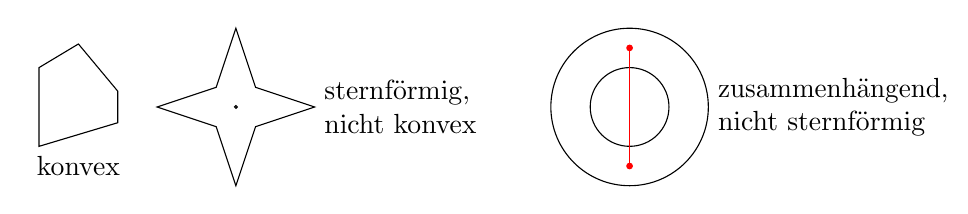
\begin{tikzpicture}

\begin{scope}
\draw (0,0) -- (0,1) -- (0.5,1.3) -- (1,0.7) -- (1,0.3) -- cycle;
\draw (0.5,0) node [below] {konvex};
\end{scope}

\begin{scope}[xshift=2.5cm,yshift=0.5cm]
\draw (0,0) circle (0.5pt);
\draw (-1,0) -- (-0.25,0.25) -- (0,1) -- (0.25,0.25) -- (1,0) -- (0.25,-0.25) -- (0,-1) -- (-0.25,-0.25) -- cycle;
\draw (1,0) node [right,text width=2.5cm] {sternförmig,\\ nicht konvex};
\end{scope}

\begin{scope}[xshift=7.5cm,yshift=0.5cm]
\draw (0,0) circle (1cm) +(0,0) circle (0.5cm);
\filldraw [red] (0,0.75) circle (1pt) (0,-0.75) circle (1pt);
\draw [red] (0,0.75) -- (0,-0.75);
\draw (1,0) node [right,text width=2.7cm] {zusammenhängend,\\ nicht sternförmig};
\end{scope}

\end{tikzpicture}
\end{center}

Klar ist: $M$ konvex \folgt $M$ sternförmig und $M$ sternförmig \folgt $M$ zusammenhängend (nach Satz~\ref{satz2.8}).

\begin{center}
\begin{tikzpicture}

\begin{scope}
\clip (-1,-1) rectangle (1,1);
\fill [red,pattern color=red,pattern=north east lines] (0,0) -- (130:1.5) -- (1,1) -- (1,-1) -- (-130:1.5) -- cycle;
\draw (0,0) -- (130:1.5) (0,0) -- (-130:1.5);
\end{scope}

\draw (0.3,0) arc (0:130:0.3);
\draw (50:0.3) node [right] {$\varphi$};

\draw (1,0) node [right=5pt,text width=7cm] {
Sektoren $\Sigma_\pi$ sind sternförmig (mit Zentrum 1) und $d$ ist konvex $\gdw \varphi<\frac{\pi}{2}$.};

\draw [->] (-1,0) -- (1.1,0);
\draw [->] (0,-1) -- (0,1.1);
\end{tikzpicture}
\end{center}

\begin{thm}[Cauchys Integralsatz für sternförmige Gebiete] \label{thm2.21}
  Seien $D\subseteq\C$ ein sternförmiges Gebiet, $f\in H(D)$ und $\Gamma\subseteq D$ eine geschlossene Kurve. Dann gilt
  \[\integral{\Gamma}{}{f}{z} = 0.\]
\end{thm}
\begin{bem*}
  Nach Satz~\ref{satz2.13} ist die Aussage von Thm.~\ref{thm2.21} äquivalent zu: Jedes $f\in H(D)$ besitzt auf $D$ eine
  Stammfunktion, wenn $D$ sternförmig ist.
\end{bem*}
\begin{proof}
  Sei $z_0$ das Zentrum von $D$. Setze für alle $z\in D$
  \[F(z) = \Integral{\overrightarrow{z_0z}}{}{f(w)}{w} = -\Integral{\overrightarrow{zz_0}}{}{f(w)}{w}.\]
  Sei $r>0$ mit $B(z,r)\subseteq D$, $z\in D$ fest, sowie $0<\abs{h}<r$. Dann:
  \begin{multline*} %TODO sieht furchtbar aus...
    \frac1h \bigl(F(z+h)-F(h)\bigr) = \frac1h \left( \Integral{\overrightarrow{z_0(z+h)}}{}{f}{w} +
      \Integral{\overrightarrow{zz_0}}{}{f}{w} + \Integral{\overrightarrow{(z+h)z}}{}{f}{w} \right) + \frac1h
    \Integral{\overrightarrow{z(z+h)}}{}{f}{w}  \\
    = \frac1h \underbrace{\Integral{\partial\Delta(z_0,z+h,z)}{}{f}{w}}_{=0 \text{ (Satz~\ref{satz2.19})}} + \underbrace{\frac1h
      \integral{0}{1}{f(z+th)h}{t}}_{\to f(z),\ h\to0 \text { nach \eqref{2.7}}}.
  \end{multline*}
  Also ist $F^\prime(z)=f(z)$.
\end{proof}

\begin{bsp} \label{bsp2.22}
  \begin{enumerate}
  \item $\displaystyle\int_{\partial\mathbb{D}}{\frac{\d z}{z+2}}=0$, denn $f(z)=\frac{1}{z+2}$ liegt in $H(D)$ für
    \[D=\{\kmplx{C} \mid \Re z > -\frac32\}.\] Beachte: $D$ ist sternförmig und offen, $\partial\mathbb{D}\subseteq D$.
  \item Cauchy ist im Allgemeinen falsch für Gebiete mit Löchern, z.B. $\C\setminus\{0\}\ad D$. Siehe Bsp.~\ref{bsp2.14}:
    $f(z)=\frac1z$, $f\in H(D)$, $\Gamma=\partial\mathbb{D}$. Dann \[\int_{\partial\mathbb{D}}{\frac{\d z}{z}} = 2\pi\i
    \neq 0.\]
  \end{enumerate}
\end{bsp}

\begin{bem*}
  Thm.~\ref{thm2.21} gilt auch, wenn $f\in C(D,\C) \cap H(D\setminus\{w_0\})$ für ein $w_0\in D$. Denn Satz~\ref{satz2.19} wurde
  für solche $f$ bewiesen.
\end{bem*}

\begin{thm}[Cauchys Integralformel für sternförmige Gebiete]
  Seien $D\subseteq\C$ ein sternförmiges Gebiet, $f\in H(D)$, $\Gamma\subseteq D$ eine geschlossene Kurve. Dann gilt
  \begin{equation} \label{CIF}
    n(\Gamma,z) f(z) = \frac{1}{2\pi\i} \integral{\Gamma}{}{\frac{f(z)}{w-z}}{w}, \quad \forall z\in D\setminus\Gamma.
    \tag{CIF}
  \end{equation}
  Speziell mit $\Gamma=\partial B(c,r)\subseteq D$ für $B(c,r)\subseteq D$ und $z\in B(c,r)$:
  \begin{align}
    \label{2.4}
    f(z) &= \frac{1}{2\pi\i} \Integral{\partial B(c,r)}{}{\frac{f(w)}{w-z}}{w} \\
    \label{2.5}
    &= \frac{1}{2\pi} \integral{0}{2\pi}{f(z+r\e^{\i t})}{t}.
  \end{align}
\end{thm}
\begin{proof}
  Sei $z\in D\setminus\Gamma$ fest. Setze $\displaystyle g(w) = \begin{cases}
    \frac{f(w)-f(z)}{w-z}, &w\in D\setminus\{z\} \\
    f^\prime(z),            &w=z.
  \end{cases}$.\\
  Dann ist $g\in C(D,\C)\cap H(D\setminus\{z\})$. Die Bemerkung nach Bsp.~\ref{bsp2.22} liefert dann
  \[ 0 = \integral{\Gamma}{}{g(w)}{w} \wegen{=}{z\notin\Gamma} \integral{\Gamma}{}{\frac{f(w)}{w-z}}{w} - f(z)
  \underbrace{\int_\Gamma{\frac{\d w}{w-z}}}_{=2\pi\i n(\Gamma,z)}. \]
  Daraus folgt \eqref{CIF} und der Spezialfall \eqref{2.4}. Mit $c=z$ und der Parametrisierung $\gamma(t)=z+r\e^{\i t}$ folgt
  aus \eqref{2.4}
  \[ f(z) = \frac{1}{2\pi\i} \integral{0}{2\pi}{\frac{f(z+r \e^{\i t})}{z+r \e^{\i t} - z}\i r\e^{\i t}}{t}, \]
  also \eqref{2.5}.
\end{proof}

\begin{bsp*}
  Es gilt $\displaystyle\Integral{\partial B(2,1)}{}{\frac{\sqrt{w}}{w-\frac32}}{w} = 2\pi\i\sqrt{\frac32}$.

  Wähle hier $D=B(2,\frac32)$, $f(w)=\sqrt{w}$. Dann ist $D$ konvex, $f\in H(D)$, $\partial B(2, 1)\subseteq D$.
\end{bsp*}

\begin{dfn} \label{dfn2.24}
  Eine Funktion $f\colon D\to\C$ heißt \emph{analytisch}, wenn es für jedes $z\in D$ eine $r(z)>0$ gibt, sodass $B(z,
  r(z))\subseteq D$ und $f$ auf $B(z,r(z))$ eine Potenzreihe mit Entwicklungspunkt $z$ und Koeffizienten $a_n(z)$ besitzt.\\
  Eine Funktion $f\in H(\C)$ heißt \emph{ganz}.
\end{dfn}

\begin{thm}[Entwicklungssatz] \label{thm2.25}
  Sei $f\in H(D)$. Dann ist $f$ analytisch auf $D$.\\
  Sei ferner $z_0\in D$ und $r>0$ mit $\bar{B}(z_0,r)\subseteq D$. Seien \nat{n}, $z\in B(z_0,r)$. Dann gelten die
  \emph{Cauchyformeln}
  \begin{equation} \label{2.6}
    f^{(n)}(z) = \frac{n!}{2\pi\i} \Integral{\partial B(z_0,r)}{}{\frac{f(w)}{(w-z)^{n+1}}}{w}
  \end{equation}
  und die \emph{Cauchy-Abschätzungen}
  \begin{equation} \label{2.7}
    \abs{f^{(n)}(z)} \leq \frac{n!}{r^n} \max_{\abs{w-z_0}=r}{\abs{f(w)}}.
  \end{equation}
  Sei $R(z_0) = \sup{\{s>0 \mid B(z_0,s) \subseteq D\}}$. Dann gilt
  \begin{equation} \label{2.8}
    f(z) = \sum_{n=0}^\infty{(z-z_0)^n\frac{1}{2\pi\i}\Integral{\partial B(z_0,r)}{}{\frac{f(w)}{(w-z_0)^{n+1}}}{w}}
    = \sum_{n=0}^\infty{\frac{f^{(n)}(z_0)}{n!}(z-z_0)^n}
  \end{equation}
  für alle $z\in B(z_0,r)$ mit $0<r<R(z_0)$. Die Reihe in \eqref{2.8} konvergiert absolut und gleichmäßig für $z\in
  B(z_0,r^\prime)$ mit $0<r^\prime<r<R(z_0)$. Wenn $f$ ganz ist, dann gibt es $a_n\in\C$ (\nat{n}), sodass
  \[ f(z) = \sum_{k=0}^\infty{a_nz^n} \quad (\forall z\in\C). \]
\end{thm}

%%%%%%%%%%%%%%%%%%%
%% Vorlesung vom 4.6.

% zu 2.25
\begin{proof}
Seien $z_0\in D$, $r > 0$ mit $\abg{B}(z_0,r)\subseteq D$. Seien $w\in\Gamma\da \partial B(z_0,r)$, $\nat{n}$, $z\in B(z_0,r)$. Dann existiert
\[\frac{\partial^n}{\partial z^n}\frac{f(w)}{w-z} = n!\frac{f(w)}{(w-z)^{n+1}}\]
und
\[(w,z)\mapsto \frac{\partial^n}{\partial z^n}\frac{f(w)}{w-z}\]
ist stetig für $w\in T$, $z\in B(z_0,r)$. Somit folgt aus der \eqref{CIF} und Satz~\ref{satz2.7}d) (mit ``$D=B(z_0,r)$''), dass $f$ auf $D$ beliebig oft differenzierbar ist und \eqref{2.6} gilt. Da $l(\Gamma) = 2\pi r$ und $(w-z_0)^{-n-1}=r^{-n-1}$, folgt \eqref{2.7} aus \eqref{2.6} (mit $z=z_0$).

Seien nun $0<r'<r$ $z\in\abg{B}(z_0,r')$. Dann gilt:
\[\frac{\abs{z-z_0}}{\abs{w-z_0}}\leq\frac{r'}{r}\ad q < 1.\]
Damit:
\[\label{2.25s}\frac{f(w)}{w-z}=\frac{f(w)}{w-z_0}\frac{1}{1-\frac{z-z_0}{w-z_0}} = \frac{f(w)}{w-z_0}\sum_{n=0}^\infty\left(\frac{z-z_0}{w-z_0}\right)^n.\tag{$*$}\]

Diese Reihe konvergiert absolut und gleichmäßig für $w\in\Gamma$ und $z\in\abg{B}(z_0,r')$. Dann gilt:
\[f(z)\!\!\nach{=}{\eqref{CIF}}\!\! \frac{1}{2\pi\i}\integral{\Gamma}{}{\frac{f(w)}{w-z}}{w} \underset{\text{Satz~\ref{satz2.7}c)}}{\overset{\eqref{2.25s}}{=}} \sum_{n=0}^\infty (z-z_0)^n\underbrace{\frac{1}{2\pi\i}\integral{\Gamma}{}{\frac{f(w)}{(w-z_0)^{n+1}}}{w}}_{\overset{\eqref{2.6}}{=}\frac{1}{n!}f^{(n)}(z_0)}.\]
Damit folgt \eqref{2.8}. Wenn $D=\C$, wähle $z =0$, $r$ beliebig groß und erhalte so letzte Bedingung.
\end{proof}

\begin{bsp}\label{bsp2.26}\begin{enumerate}
\item Das Theorem ist falsch im Reellen, Beispiel aus Analysis 1:
\begin{enumerate}
\item $\displaystyle f(x)=\begin{cases}x^{\frac{3}{2}}\sin\frac{1}{x},&x>0,\\0,&x\leq 0.\end{cases}\folgt$ $f$ ist differenzierbar auf $\R$ (mit $f^\prime(0) = 0$) \textit{aber} $f^\prime$ ist unbeschränkt für $x\ra 0_+$, also unstetig und $\nexists f^{\prime\prime}$.

\item $\displaystyle f(x)=\begin{cases}\e^{-\frac{1}{x^2}},&x>0,\\0,&x\leq0.\end{cases}\leadsto f\in C^\infty(\R)$ aber $f^{(n)}(0)=0$ $(\forall\nat{n})$, als Taylorreihe von $f$ in $0$ ist konstant 0, also ungleich $f$.
\end{enumerate}
\item Sei $f(z)=(1+z)^\alpha$ (wobei $\reell{\alpha}$ fest, $z\in D = \C\setminus(-\infty,-1]$) $\leadsto f$ ist holomorph auf $D$. Aus Theorem~\ref{thm2.25} folgt: $f$ hat Potenzreihe in $z_0=0$. Diese ist gleich der Binomialreihe aus Analysis 1. Nach Theorem~\ref{thm2.25} ist der Konvergenzradius $\rho\geq 1$. \textit{Falls} $\rho <1$ hätten alle Ableitungen von $f$ eine stetige Fortsetzung auf $\partial B(0,1)$. Das widerspricht der Definition von $f\folgt\rho=1$.
\end{enumerate}
\end{bsp}

\begin{kor}\label{kor2.27}
Gegeben sei eine Borelmenge $X\subseteq\R^d$ und eine Funktion $h\colon D\times X\to\C$, wobei $D\subseteq\C$ offen, mit:
\begin{enumerate}
\item $\forall z\in D$ ist $x\mapsto h(z,x)$ integrierbar auf $X$.
\item $\forall x\in X$ ist $z\mapsto h(z,x)$ holomorph auf $D$.
\item Es existiert ein integrierbares $g\colon X\to\R_+$ mit $\abs{h(z,x)}\leq g(x)$ $(\forall z\in D,\ x\in X)$. Dann ist
\[z\mapsto H(z)\da \integral{X}{}{h(z,x)}{x}\]
holomorph auf $D$ und es gilt:
\[H^{(k)}(z)=\integral{X}{}{\frac{\partial^k}{\partial z^k}h(z,x)}{x}\quad(\forall\nat{k}).\]
\end{enumerate}
\end{kor}

\begin{proof} Sei $z_0\in D$, $r>0$ fest (aber beliebig) mit $B(z_0,r)\subseteq D$. Sei $z\in B(z_0,r)\!\!\!\folgt\!\!\!\abg{B}(z_0,r)\subseteq D$. \eqref{2.7} für $z$ und $\nat{k}$ liefert
\[\label{2.27s}\abs{\frac{\partial^k}{\partial z^k}h(z,x)}\leq \frac{k!}{r^k}\max_{\abs{w-z}=r}\abs{h(w,x)}\overset{\text{n.V.}}{\leq}\frac{h!}{r^k}g(x)\quad\text{(für jedes feste $x\in X$.)}\tag{$*$}\]

Seien nun $z_n\ra z_0$, mit $z_n\in B(z_0,r)\setminus\{z_0\}$ $(\forall\nat{n})$. Dann:
\begin{gather*}
D_n\da \frac{1}{z_n-z_0}\Bigl(H(z_n)-H(z_0)\Bigr) = \integral{X}{}{\frac{1}{z_n-z_0}\Bigl(h(z_n,x)-h(z_0,x)\Bigr)}{x}\\
\overset{\eqref{2.1}}{=}\integral{X}{}{\frac{1}{z_n-z_0}\integral{0}{1}{\underbrace{\left(\frac{\partial}{\partial z}h\right)\Bigl(z_0+t(z_n-z_0),x\Bigr)}_{\ad\varphi_n(t,x)}\cdot\,(z_n-z_0)}{t}}{x}
\end{gather*}
(Vergleiche hierzu das Vorgehen im Beweis zu Satz~\ref{satz2.7}d)).

{Es gilt:} $\varphi_n(t,x)\ra\frac{\partial}{\partial z}h(z_0,x)$ $(n\ra+\infty)$ gleichmäßig in $t\in[0,1]$, für jedes feste $x\in X$, da
\[z\mapsto\frac{\partial}{\partial z}h(z,x)\]
stetig ist nach Theorem~\ref{thm2.25}. Also:
\[\integral{0}{1}{\varphi_n(t,x)}{t}=\frac{\partial}{\partial z}h(z_0,x)\quad(n\ra+\infty,\ x\in X).\]
Ferner:
\[\abs{\integral{0}{1}{\varphi_n(t,x)}{t}}\overset{*}{\underset{(k=1)}{\leq}}\frac{1}{r}g(x)\quad(\forall\nat{n},\ x\in X),\]
wobei $g(x)$ integrierbar ist.
Majorisierte Konvergenz liefert:
\[D_n\longrightarrow\integral{X}{}{\frac{\partial}{\partial z}h(z_0,x)}{x}\quad(n\ra\infty).\]
$\folgt H$ ist bei $z_0$ differenzierbar $\folgt H\in H(D)$. Ferner:
\[H^\prime(z) = \integral{X}{}{\frac{\partial}{\partial z}h(z,x)}{x}\quad(\forall z\in D).\]
Beachte: $\frac{\partial}{\partial z}h(z,x)$ ist in $x$ messbar, also liefern Theorem~\ref{thm2.25} und \eqref{2.27s} eine iterative Formel für $H^{(k)}$.
\end{proof}

\begin{bsp}[Laplacetransformation]\label{bsp2.28}
Sei $f\colon\R_+\ra\C$ messbar, so dass für gewisse $w\in\R$, $c>0$ gilt:
\[\abs{f(t)}\leq c\e^{wt}\quad(\forall t\geq 0).\]
Dann:
\[\exists\hat{f}(\lambda)=\integral{0}{\infty}{\e^{-\lambda t}f(t)}{t}\]
für $\lambda\in\C$ mit $\Re{\lambda}>w$ und ist dort holomorph mit
\[\hat{f}(\lambda)^{(n)}=(-1)^n\integral{0}{\infty}{\e^{-\lambda t}t^n f(t)}{t}\quad(\forall\lambda\text{ mit }\Re{\lambda}>w,\ \nat{n}).\]

\begin{proof} Setze
\[h(\lambda, t)=\e^{-\lambda t}f(t)\quad\text{für }t\geq 0,\ \Re{\lambda}>w.\]
Klar: $h$ ist in $\lambda$ holomorph $(\forall t\geq 0)$.

Sei $\ep >0$ fest aber beliebig, $\Re{\lambda}\geq w+\ep > w$. Dann:
\[\abs{h(\lambda,t)}=\e^{-\Re{\lambda}t}\abs{f(t)}\leq\e^{-wt}\e^{-\ep t}\abs{f(t)}\overset{\text{n.V.}}{\leq}c\e^{-\ep t}\ad g(t),\]
wobei $g(t)$ integrierbar und unabhängig von $\lambda$ ist.

Korollar~\ref{kor2.27} liefert Holomorphie von $\hat{f}(\lambda)$ für $\Re{\lambda}\geq w+\ep$, folglich die Holomorphie für $\Re{\lambda}>w$, da $\ep>0$ beliebig. Weiter gilt:
\[\hat{f}(\lambda)^{(n)}=\integral{0}{\infty}{\left(\frac{\d}{\d\lambda}\right)^n\e^{-\lambda t}f(t)}{t}=(-1)^n\integral{0}{\infty}{t^n\e^{-\lambda t}f(t)}{t}\quad(\Re{\lambda}>w).\qedhere\]
\end{proof}
\end{bsp}

\begin{kor}[Morera]\label{kor2.29}
Sei $f\in C(D,\C)$ so dass
\[\integral{\partial\Delta}{}{f}{z}=0\]
für alle Dreiecke $\Delta\subseteq D$. Dann: $f\in H(D)$.
\end{kor}

\begin{proof} Sei $z\in D$. Wähle $r>0$ mit $B(z,r)\subseteq D$. Nach dem Beweis von Theorem~\ref{thm2.21} impliziert die Vorraussetzung, dass $f$ auf $B(z,r)$ (sternförmig) eine Stammfunktion $F\in H(B(z,r))$ besitzt. Nach Theorem~\ref{thm2.25} ist $F\in C^2$ und somit ist $f=F^\prime$ differenzierbar auf $B(z,r)$. Daraus folgt die Behauptung.
\end{proof}


%%% Vorlesung vom 8. Juni
\begin{thm}[Liouville] \label{thm2.30}
  Eine beschränkte ganze Funktion ist konstant.
\end{thm}
\begin{proof}
  Sei $f$ eine beschränkte ganze Funktion und \kmplx{z}. \eqref{2.7} mit $n=1$ liefert:
  \[ \abs{f^\prime(z)} \leq \frac1r \max_{\abs{z-w}=r}{\abs{f(w)}} \leq \frac1r \Vert f \Vert _\infty, \]
  wobei hier $r>0$ beliebig ist, da $f\in H(\C)$. Mit $r\to\infty$ folgt $f^\prime(z)=0$ für alle \kmplx{z}. Nach Satz~\ref{satz2.10} ist $f$ konstant.
\end{proof}

\begin{kor}[Fundamentalsatz der Algebra] \label{kor2.31}
  Ein Polynom $p(z)=a_nz^n+\dotsb+a_1z+a_0$ (mit $\kmplx{a_k}\ (k=1,\dotsc,n)$, $a_n\neq0$, \kmplx{z}) hat genau $n$ (eventuell mehrfach gezählte) Nullstellen.
\end{kor}
\begin{proof}
  Sei $p(z)\neq0$ für alle \kmplx{z}. Wir zeigen, dass $p$ konstant ist. Setze dazu $f=\frac1p\in H(\C)$. Wähle $r>0$, sodass
  \[ \sum_{j=0}^{n-1}{\frac{\abs{a_j}}{\abs{a_n}}\abs{z}^{j-n}} \le \frac12 \quad \text{für alle $z$ mit } \abs{z} \ge r. \]
  Sei $\abs{z} \ge r$. Dann gilt
  \[ \abs{p(z)} \ge \abs{a_n}\abs{z}^n - \left(\abs{a_{n-1}}\abs{z}^{n-1} + \dotsb + \abs{a_0}\right) =
  \abs{a_n}\abs{z}^n \left(1-\sum_{j=0}^{n-1}{\frac{\abs{a_j}}{\abs{a_n}}\abs{z}^{j-n}} \right) \ge
  \frac12\abs{a_n}r^n.\]
  Also ist $f(z)\le \frac{2}{\abs{a_n}r^n}$, wenn $\abs{z}\ge r$. Ferner ist $f$ auf $\bar{B}(0,r)$ beschränkt als stetige
  Funktion auf einer kompakten Menge. Damit ist $f$ beschränkt auf ganz $\C$. Mit Liouville (Thm.~\ref{thm2.30}) folgt, dass $f$
  und damit auch $p$ konstant ist.

  Damit hat jedes nichtkonstante Polynom, d.h. jedes Polynom vom Grad $\ge1$ mindestens eine Nullstelle. Mit Polynomdivision
  folgt induktiv die Behauptung.
\end{proof}

\begin{dfn} \label{dfn2.32}
  Sei $U\subseteq\mathbb{K}^l$ offen (wobei $\mathbb{K}\in\{\R,\C\}$) und $f,f_n\colon U\to\mathbb{K}^k$ Funktionen für alle
  \nat{n}. Man sagt, dass $f_n\to f$ für \ninf \ \emph{kompakt konvergiert} (oder "`\emph{gleichmäßig auf kompakten Mengen}"'),
  wenn für jede kompakte Menge $K\subseteq U$ gilt: \[ \sup_{x\in K}{\abs{f(x)-f_n(x)}_2}\to0 \quad (\ninf). \]
\end{dfn}

\begin{bem} \label{bem2.33}
  \begin{enumerate}
  \item Sei $f_n\to f$ (kompakt) und $f_n$ stetig für jedes \nat{n}. Nach Analysis 2 ist dann $f$ stetig auf $K$ für jedes
    kompakte $K$, z.B. $K=\bar{B}(x,r)\subseteq U$. Also ist $f\in C(U,\mathbb{K}^k)$. Im Reellen folgt aber selbst aus $f_n\in
    C^\infty$ nicht, dass $f\in C^1$. Gegenbeispiel aus Analysis 2: $f_n(x) = \sqrt{\frac{1}{n^2}+x^2}$ für $x\in(-1,1)$. Hier
    ist $f_n\in C^\infty((-1,1))$ für alle \nat{n} und $f_n\to f$ (\ninf) gleichmäßig auf $(-1,1)$ mit $f(x)=\abs{x}$. Aber $f$
    ist bei $0$ nicht differenzierbar. %TODO Bild (?)
  \item Die Partialsummen einer Potenzreihe $f(z)=\sum_{n=0}^\infty{a_n(z-z_0)^n}$ mit Konvergenzradius $\rho$ konvergieren
    kompakt auf $B(z_0,\rho)$ gegen $f$. Im Allgemeinen haben wir aber keine gleichmäßige Konvergenz auf $B(z_0,\rho)$.
    \begin{proof}
      Sei $K\subseteq B(z_0,\rho)$ kompakt. Nach Satz vom Maximum existiert ein $z_1\in K$ mit
      \[ \abs{z_0-z_1} = \max_{z\in K}{\abs{z_0-z}} \ad r < \rho, \]
      da $z_1\in K\subseteq B(z_0,\rho)$. Also gilt $K\subseteq\bar{B}(z_0,r)\subseteq B(z_0,\rho)$. Ferner:
      \[ \max_{z\in\bar{B}(z_0,r)}{\abs{a_n}\abs{z-z_0}^n} \le \abs{a_n}r^n \ad b_n \quad (\forall\nat{n}), \]
      \[ \ls_{\ninf}{\sqrt[n]{b_n}} = r\ls_{\ninf}{\sqrt{\abs{a_n}}} = \frac{r}{\rho} < 1. \]
      Nach dem Wurzelkriterium gilt dann $\sum_{n=0}^\infty{b_n}<\infty$. Satz 1.13 (Weierstraß) aus Analysis 2 impliziert, dass
      die Potenzreihe gleichmäßig und absolut auf $\bar{B}(z_0,r)$ konvergiert, und somit auf $K$.
    \end{proof}
  \end{enumerate}
\end{bem}

\begin{thm}[Konvergenzsatz von Weierstraß] \label{thm2.34}
  Seien $f_n\in H(D)$ für \nat{n} und $f_n\to f$ (kompakt) für ein $f\in C(D,\C)$ (\ninf). Dann gilt $f\in H(D)$ und $f_n^{(j)}$
  konvergiert kompakt gegen $f^{(j)}$ für \ninf und jedes \nat{j}.
\end{thm}
\begin{proof}
  Sei $\Delta\subseteq D$ ein abgeschlossenes Dreieck. Dann gilt $f_n\to f$ (gleichmäßig) auf $\partial\Delta\subseteq D$
  (\ninf). Damit:
  \[ 0 \nach{=}{\ref{satz2.19}} \Integral{\partial\Delta}{}{f_n}{z} \nach{\longrightarrow}{\ref{satz2.7}}
  \Integral{\partial\Delta}{}{f}{z} \ (\ninf)
  \quad \folgt \quad \Integral{\partial\Delta}{}{f}{z} = 0. \]
  Nach Morera (Kor.~\ref{kor2.29}) gilt dann $f\in H(D)$.

  Sei $r>0$, $z_0\in D$ mit $\bar{B}(z_0,2r)\subseteq D$. Sei $z\in\bar{B}(z_0,r)$. Dann gilt
  $\bar{B}(z,r)\subseteq\bar{B}(z_0,2r)$. Da $f-f_n\in H(D)$, folgt mit \eqref{2.7}, dass
  \begin{align*} \label{thm2.34_stern}
    \max_{z\in\bar{B}(z_0,r)}{\abs{f^{(j)}(z)-f_n^{(j)}(z)}} & \le
    \max_{z\in\bar{B}(z_0,r)}{\max_{\abs{w-z}=r}{\frac{j!}{r^j}\abs{f(w)-f_n(w)}}} \\ & \le
    \frac{j!}{r^j} \max_{\abs{w-z}\le2r}{\abs{f(w)-f_n(w)}} \\ & \longrightarrow 0\ (\ninf) \text{ nach Voraussetzung,} \tag{$*$}
  \end{align*}
  also $f_n^{(j)} \to f^{(j)}$ auf $\bar{B}(z_0,r)$ (\ninf, \nat{j}).

  Sei $K\subseteq D$ kompakt. Dann gibt es für jedes $z_0\in K$ ein $r(z_0)>0$ mit $B(z_0,2r(z_0))\subseteq D$, da $D$ offen. Klar:
  \[ K \subseteq \bigcup_{z_0\in K}{B(z_0,r(z_0))}. \] Da $K$ kompakt ist, existieren endlich viele $z_1,\dotsc,z_m\in K$ und
  $r_1,\dotsc,r_m>0$ mit $B(z_k,2r_k)\subseteq D$ ($k=1,\dotsc,m$) und $K\subseteq B(z_1,r_1)\cup\dotsb\cup
  B(z_m,r_m)$. \eqref{thm2.34_stern} angewandt auf $\bar{B}(z_k,r_k)$ liefert die Behauptung.
\end{proof}



\section{Weitere Hauptsätze über holomorphe Funktionen}

\begin{thm}[Identitätssatz]\label{thm2.35}
  Sei $D\subseteq\C$ ein Gebiet und $f\in H(D)$. Dann sind äquivalent:
  \begin{enumerate}
  \item $f=0$ auf $D$.
  \item Es gibt ein $z_0\in D$ mit $f^{(m)}(z_0)=0$ für alle \nat{m}.
  \item $N=\{ z\in D \mid f(z)=0 \}$ hat einen Häufungspunkt $z_0\in N$, d.h. es gibt eine Folge $z_n\in D\setminus\{z_0\}$
    (\nat{n}) mit $z_n\to z_0$ und $z_n\in N$.
  \end{enumerate}
  Somit sind zwei Funktionen $g,h\in H(D)$ schon gleich, sobald $g(z_n)=h(z_n)$ auf einer Folge $z_n\to z_0$ mit $z_n,z_0\in D$
  und $z_n\neq z_0$ (\nat{n}) oder sobald für ein $z_0\in D$ gilt: $g^{(m)}(z_0)=h^{(m)}(z_0)$ für alle
  $m\in\mathbb{N}_0$. Insbesondere sind die Koeffizienten einer Potenzreihe eindeutig bestimmt.
\end{thm}
\begin{bem*}
  Der Satz ist falsch, wenn $D$ nicht zusammenhängend ist.
\end{bem*}
\begin{proof}
  Die letzte Behauptung folgt mit $f=g-h$ aus "`(c)$\Rightarrow$(a)"' bzw. "`(b)$\Rightarrow$(a)"'.
  \begin{enumerate}
  \item[a)]$\!\Rightarrow$ c): klar.
  \item[c)]$\!\Rightarrow$ b): Seien $z_n,z_0\in D$, $z_n\neq z_0$, $f(z_n)=0$ ($\forall\nat{n}$), $z_n\to z_0$ (\ninf). Dann
    ist $f(z_0) = 0$.

    Annahme: Es gibt ein \nat{m} mit $f(z_0)=f^\prime(z_0)=\dotsb=f^{(m-1)}(z_0)=0$ und $f^{(m)}(z_0)\neq0$. Thm.~\ref{thm2.25}
    liefert ein $r>0$ mit
    \[ f(z)=\sum_{k=m}^\infty{\underbrace{\frac{f^{(k)}(z_0)}{k!}}_{\ad a_n}(z-z_0)^k}\qquad(\forall z\in B(z_0,r)\subseteq D),\]
    wobei $a_m\neq0$. Damit:
    \[ g(z) \da (z-z_0)^{-m}f(z) = \sum_{k=m}^\infty{a_k(z-z_0)^{k-m}} \wegen{=}{l=k-m} \sum_{l=0}^\infty{a_{l+m}(z-z_0)^l}
    \quad (z\in B(z_0,r)).\]
    Also ist $g\in H(B(z_0,r))$ und $g(z_0)=a_m\neq0$. Aber $g(z_n)=(z_n-z_0)^{-m}f(z_0)=0$, wobei $z_n\neq z_0$, $z_n,z_0\in
    B(z_0,r)$ und $z_n\to z_0$ (\ninf). $\blitz$ zu c). \folgt b) gilt.
  \item[b)]$\!\Rightarrow$ a): \qedhere
  \end{enumerate}
\end{proof}

% Vorlesung vom 18.6.09
%Bew zu 2.41:
\begin{proof} Sei $U\subseteq D$ offen, $z_0\in U$ fest, aber 
beliebig. Nach Korollar~\ref{kor2.37} (mit ``$c=f(z_0)$'') existiert 
ein $r>0$ mit $f(z)\neq f(z_0)$ für alle $z\in\abg{B}(z_0,r)\ad B
\subseteq U$ mit $z\neq z_0$. Da $\partial B$ kompakt, folgt
\[\exists\frac{1}{2}\min_{z\in\partial B}\abs{f(z)-f(z_0)}\ad\delta >0.\]
Sei nun $w\in B(f(z_0),\delta)$ beliebig, aber fest. Dann ist zu 
zeigen: $w\in f(U)$. Dies ist genau dann der Fall, wenn
\[\exists z_1\in U: f(z_1)=2.\]
Für $z\in\partial B$ gilt:
\begin{gather*}\abs{f(z)-w}\geq\abs{f(z)-f(z_0)}-\abs{f(z_0)-w}\geq 
2\delta - \delta = \delta\\
\folgt \min_{z\in\partial B}\abs{f(z)-w}\geq\delta.\end{gather*}
Lemma~\ref{lem2.40} für $g\da f-w$ liefert $z_1\in B(z_0,r)
\subseteq U$ mit $g(z_1)=0\gdw f(z_1)=w$. Also ist $f(U)$ offen. 
Wenn $U$ zusammenhängend ist, dann ist $f(U)$ nach Theorem~1.68 (Ana 2) zusammenhängend.
\end{proof}

\begin{thm}[Maximumsprinzip]\label{thm2.42}
Seien $D\subseteq\C$ ein Gebiet und $f\in H(D)$ nicht konstant.
\begin{enumerate}
\item\label{thm2.42a} Dann hat die Funktion $z\mapsto\abs{f(z)}$ kein lokales Maximum auf $D$.
\item\label{thm2.42b} Wenn ferner $f\in C(\abg{D},\C)$ und $D$ beschränkt ist, dann gilt:
\[\max_{z\in\abg{D}}\abs{f(z)}=\max_{z\in\partial D}\abs{f(z)}.\]
\end{enumerate}
\end{thm}

\begin{proof}\begin{enumerate}
\item Annahme: $\exists\, z_0\in D$, $r>0$ mit $\abs{f(z)}\leq\abs{f(z_0)}$ $(\forall z\in B(z_0,r)\subseteq D)$.

Wähle $w_n\in\C$ mit $\abs{w_n}>\abs{f(z_0)}$ mit $w_n\to f(z_0)$ $(n\to+\infty)$. Nach Theorem~\ref{thm2.41} ist $f(B(z_0,r))$ offen, also
\[\label{2.42s}\exists\,\delta>0: B(f(z_0),\delta)\subseteq f(B(z_0,r)).\tag{$*$}\]
Wähle $\nat{N}$ mit $w_n\in B(f(z_0),\delta)$. Dann folgt mit \eqref{2.42s}:
\[\exists\, z\in B(z_0,r)\text{ mit }f(z)=w_n\folgt\abs{f(z)}=\abs{w_n}>\abs{f(z_0)}\quad\blitz\]

\item Nach Vorraussetzung gibt es $z_1\in\abg{D}$ mit
\[\abs{f(z_1)} = \max_{z\in\abg{D}}\abs{f(z)}.\]
Nach \hyperref[thm2.42a]{a)} gilt $z_1\in\partial D$.\qedhere
\end{enumerate}
\end{proof}

\begin{bem*} Theorem~\ref{thm2.42b} ist im allgemeinen falsch für unbeschränkte Gebiete. \textit{Beispiel}:
\[D=\{z\in\C\colon -\frac{\pi}{2}<\Im{z}<\frac{\pi}{2}\},\quad f(z)=\exp(\exp(z)).\]
Dann ist $f\in H(\C)$ und für $x\in\R$ gilt $x\pm\i\frac{\pi}{2}\in\partial D$,
\[\abs{f\biggl(x\pm\i\frac{\pi}{2}\biggr)}=\bigl\lvert\exp(\e^x\underbrace{\e^{\pm\i\frac{\pi}{2}}}_{=\pm\i})\bigr\rvert=1.\]
Aber $\exp(\exp(x))$ ist unbeschränkt!.
\end{bem*}

\begin{bsp}[Potenzreihenentwicklung für gewöhnliche Differentialgleichungen] (allgemeines in Walter: Gewöhnliche DGL) Wir haben Lösungen von
\[\label{2.43s}\begin{cases}u^{\prime\prime}(x)+b(x)u^\prime(x)+a(x)u(x)=0,\quad x\in\R\\u(0)=u_0,\quad u^\prime(0)=u_1.\end{cases}\tag{$*$}\]
\paragraph{Frage:} Hat $u$ eine Potenzreihe? Einfache Antwort mittels Holomorphie!
\vspace*{-12pt}\paragraph{Voraussetzung:} Sei $D\subseteq\C$ ein Gebiet mit $0\in D$, $a,\,b\in H(D)$ und $R>0$ mit $\abg{B}(0,R)\subseteq D$. Setze
\[\label{2.43ss}M\da\max_{\abs{z}\leq R}\{\abs{a(z)},\,\abs{b(z)}\}.\tag{$**$}\]
Seien $u_0,\,u_1\in\C$ gegeben, löse:
\begin{equation}\label{2.9}\begin{cases}
u^{\prime\prime}(z)+b(z)u^\prime(z)+a(z)u(z)=0,\quad z\in D,\\
u(0)=u_0,\quad u^\prime(0)=u_1.
\end{cases}\end{equation}
Sei $f\in H(B(0,R))$, $r\leq R$. Setze
\[\integral{0}{z}{f(w)}{w}=\Integral{\overrightarrow{DZ}}{}{f(w)}{w},\quad\abs{z}<r.\]
Dann
\[\exists\,\frac{\d}{\d z}\integral{0}{z}{f(w)}{w}=\!\!\!\lim_{\substack{h\to 0\\(h\neq 0,\,\abs{z+h}<r)}}\!\!\!\frac{1}{h}\left(\Integral{0}{z+h}{\!\!f}{w}-\Integral{0}{z}{f}{w}\right)=\lim_{h\to 0}\frac{1}{h}\Integral{z}{z+h}{\!f}{w}\underset{\substack{\text{vgl. Bew.}\\\text{von \ref{satz2.13}}}}{=}f(z).\]

Damit und mit Satz~\ref{satz2.13} folgt:
\[\eqref{2.9}\gdw\begin{cases}u(z)=u_0+\displaystyle\integral{0}{z}{\!u^\prime(w)}{w}\\u^\prime(z)=u_1-\displaystyle\integral{0}{z}{\!\bigl(a(w)u(w)+b(w)u^\prime(w)\bigr)}{w}.\end{cases}\]
Mit ``$v=u^\prime$'' definiere
\[\biggl(T(u,v)\biggr)(z)=\biggl(u_0+\integral{0}{z}{\!v(w)}{w},\, u_1-\integral{0}{z}{\!(au+bv)}{w}\biggr)\]
für $r<\min\{R,1,\frac{1}{2M}\}$, $z\in B(0,r)$, $(u,v)\in H(B(0,R))^2\cap C(\abg{B}(0,R))^2\ad E$.

Setze $q=\min\{r,2m\}<1$. Dann: $T(u,v)\in E$ und $E$ ist ein Vektorraum mit Norm
\[\|(u,v)\|_\infty=\max_{\abs{z}\leq r}\{\abs{u(z)},\,\abs{v(z)}\}.\]

\vspace*{-20pt}\paragraph{Beh.:} $(E,\|\cdot\|)$ ist vollständig.
\begin{proof} Sei $(u_n,v_n)$ eine Cauchyfolge in $E$. $\folgt (u_n),\,(v_n)$ sind Cauchyfolgen in $C(\abg{B}(0,r))$ bezüglich der Supremumsnorm. Dies ist ein Banachraum (Ana 2).
\[\folgt\exists\, u,v\in C(\abg{B}(0,r))\text{ mit }u_n\to u,\,v_n\to v\text{ gleichmäßig auf }\abg{B}(0,r).\]
Aus Theorem~\ref{thm2.34} folgt: $u,v\in H(B(0,r))$. Beachte:
\[\|(u_n,v_n)-(u,v)\|_\infty\lra 0,\quad n\to +\infty.\qedhere\]
\end{proof}

Seien $(u,v)$, $(\tilde{u},\tilde{v})\in E$. Dann:
\begin{align*}
\|T(u,v)-T(\tilde{u},\tilde{v})\|_\infty=&\,\max_{\abs{z}\leq r}\biggl\{\abs{\integral{0}{z}{\bigl(v(w)-\tilde{v}(w)\bigr)}{w}},\\
&\qquad\qquad\qquad\abs{\integral{0}{z}{\biggl(a(w)(u(w)-\tilde{u}(w))+b(w)(v(w)-\tilde{v}(w))\biggr)}{w}}\biggr\}\\
\overset{\eqref{2.43ss}}{\leq}&\max_{\abs{w}\leq\abs{z}\leq r}\{\underset{\leq r}{\abs{z}}\abs{v(w)-\tilde{v}(w)},\,\underset{\leq r}{\abs{z}}(M\abs{u(w)-\tilde{u}(w)}+M\abs{v(w)-\tilde{v}(w)})\}\\
\leq\, &\:\;r\underbrace{\max\{r,2M\}}_{=q<1}\|(u,\tilde{u})-(v,\tilde{v})\|_\infty
\end{align*}

Banachscher Fixpunktsatz: $\exists!\,(u,v)=T(u,v)\folgt u$ löst \eqref{2.9} auf $B(0,r)$.

Aus Theorem~\ref{thm2.25} folgt $\exists\, c_n\in\C,\, n\in\N_0$ mit 
\begin{equation}\label{2.10}\begin{cases}
u(z)=\sum_{n=0}^{+\infty}c_n z^n,\quad\forall z\in B(0,r)\\
c_0=u_0,\quad c_1=u_1.
\end{cases}\end{equation}
Ein Beispiel zur Berechnung von $c_n$: \textbf{Hermitesche DGL:}

Gegeben: $\lambda\in\R$, $u_0,\,u_1\in\R$.
\begin{equation}\label{2.11}\begin{cases}
u^{\prime\prime}(x)-2xu^\prime(x)+\lambda u(x)=0\\
u(0)=u_0,\quad u^\prime(0)=u_1.
\end{cases}\end{equation}
Hier ist $a(z)=\lambda$, $b(z)=-2z$ $(z\in\C)$. Dann folgt nach Satz~\ref{satz1.3}
\begin{gather*}
-2zu^\prime(z)=-2z\sum_{n=1}^{+\infty}nc_nz^{n-1}=\sum_{n=1}^{+\infty}(-2nc_n)z^n,\\
u^{\prime\prime}=\sum_{n=2}^{+\infty}n(n-1)c_nz^{n-2}\overset{k=n-2}{=}\sum_{k=0}^{+\infty}(k+2)(k+1)c_{k+2}z^k
\end{gather*}
für ein $z\in B(0,r)$, $r$ aus \eqref{2.10}. Dann folgt aus \eqref{2.11}
\begin{gather*}
\sum_{n=0}^{+\infty}\bigl[(n+1)(n+2)c_{n+2}-2nc_n+\lambda c_n\bigr]z^n=0,\quad c_0=u_0,\,c_1=u_1.\\
\folgtwegen{\ref{thm2.35}}\begin{cases}(n+1)(n+2)c_{n+2}-2nc_n+\lambda c_n=0,\quad n\in\N_0,\\c_0=u_0,\quad c_1=u_1.\end{cases}\folgt c_{n+2}=\frac{2n-\lambda}{(n+1)(n+2)}c_n\\
\folgt c_k = \begin{cases}
\frac{1}{k!}(2(k-2)-\lambda)(2(k-4)-\lambda)\dotsm(-\lambda)c_0,&k\text{ gerade,}\\
\frac{1}{k!}(2(k-2)-\lambda)\dotsm(2-\lambda)c_1),&k\text{ ungerade.}\end{cases}
\end{gather*}

Zwei linear unabhängige Lösungen erhält man durch:

\begin{enumerate}[label=\arabic*)]
\item $c_0=u_0=1$, $c_1=u_1=0$; Lösung:
\[v_{1,\lambda}(x)=1-\frac{\lambda}{2!}x^2-\frac{4-\lambda}{4!}x^4-\frac{(8-\lambda)(4-\lambda)}{6!}x^6-\dotso\]
\item $c_0=0$, $c_1=1$; Lösung:
\[v_{2,\lambda}(x)=x+\frac{2-\lambda}{3!}x^3+\frac{(6-\lambda)(2-\lambda)}{5!}x^5+\dotso\]
\end{enumerate}

Wenn $\lambda=2m$, $m\in\N_0$: Abbruch der Rekusion wenn
\begin{itemize}
\item[] \textbf{Fall 1:} $m$ gerade, $u_0=1$, $u_1=0$,
\item[] \textbf{Fall 2:} $m$ ungerade, $u_0=0$, $u_1=1$.
\end{itemize}

\vspace*{-16pt}
\begin{align*}
\lambda=0,\,m=0\colon\,&u_0(x)=1\\
\lambda=2,\,m=1\colon\,&u_1(x)=x\\
\lambda=4,\,m=2\colon\,&u_2(x)=1-2x^2\\
\lambda=6,\,m=3\colon\,&u_3(x)=x-\frac{2}{3}x^3
\end{align*}

Diese Lösungen erfüllen
\[\label{2.43+}\integral{\R}{}{\e^{-x^2}\abs{u_n(x)}^2}{x}<\infty\tag{+}\]
Man kann zeigen, dass alle anderen Lösungen von \eqref{2.11} \eqref{2.43+} verletzen.
\end{bsp}

%%%%%%%%%%%%%%%%%%%%
%%% Korrektur zu 3.3c!
% $z_0$ wesentlich $\gdw \forall r>0$ mit $D_0=B(z_0,r)\setminus\{z_0\}\subseteq D$ gilt $\abg{f(D_0)}=\C$.
%%%%%%%%%%%%%%%%%%%%%%

\chapter{3 halt ...}

%%%%%%%%%%%%%%%%%%%%%%%%%%
%VL vom 24.6.

Zusatz zu Theorem~\ref{thm3.5}: Wenn $f\colon D\to f(D)$ biholomorph, dann gilt nach Satz~\ref{satz1.8a}:
\[f^\prime(z)\neq 0\quad(\forall z\in D),\qquad\bigl(f^{-1}\bigr)(w)=\frac{1}{f^\prime\bigl(f^{-1}(w)\bigr)}\quad(w\in f(D)).\]

Seien $a_n\in\C$ $(n\in\Z)$ und $z_0\in\C$ gegeben. Wir sagen, dass die \textit{Laurentreihe}
\[\sum_{n=-\infty}^{+\infty}a_n(z-z_0)^n\]
für ein $z\in\C$ konvergiert, wenn ihr \textit{regulärer Anteil}
\[\sum_{n=0}^{+\infty}a_n(z-z_0)^n\]
und ihr \textit{singulärer Anteil}
\[\sum_{n=1}^{+\infty}a_{-n}(z-z_0)^{-n}\]
konvergiert. Die Laurentreihe ist dann die Summe der beiden Anteile. Entsprechend definiert man absolute beziehungsweise gleichmäßige Konvergenz auf Kompakta.

\begin{thm}[Laurent]\label{thm3.6}
Seien $f\in H(D)$, $z_0\in\C$, $R>0$ mit $D_0=B(z_0,R)\setminus\{z_0\}\subseteq D$. Für $\rho\in(0,R)$, setze
$K_\rho=\partial B(z_0,\rho)$ und
\begin{equation}\label{3.1}
a_n=\frac{1}{2\pi\i}\integral{K_\rho}{}{\frac{f(w)}{w-z_0)^{n+1}}}{w},\quad n\in\Z
\end{equation}
Dann gilt:
\begin{equation}\label{3.2}
f(z)=\sum_{n=-\infty}^{+\infty}a_n(z-z_0)^n\text{ für }z\in D_0
\end{equation}
mit absoluter und gleichmäßiger Konvergenz auf Kompakta in $D_0$. Die Koeffizienten $a_n$ sind dabei eindeutig bestimmt, insbesondere sind sie unabhängig von $\rho$.
\end{thm}

\begin{proof}
\begin{enumerate}[label=\arabic*)]
\item\label{thm3.6:1} \textit{Existenz:} Sei $K\subseteq D_0$ kompakt. Dann existieren
\[0<s<s+\delta<r-\delta<r<R\text{ mit }s+\delta\leq\abs{z-z_0}\leq r-\delta,\quad\forall z\in K\]
(vgl. den Beweis von Theorem~\ref{thm2.25}). Wähle ein $z\in K$. Setze
\[\theta=\arg(z-z_0),\quad S_\varphi=\{z_0+ t\e^{\i\varphi},\ s\leq t\leq r\}\]
für $\varphi\in\R$ und
\[K_\sigma^1=\left\{z=z_0+\sigma\e^{\i\alpha}: \theta-\frac{\pi}{2}\leq\alpha\leq\theta+\frac{\pi}{2}\right\},\quad K_\sigma^2=K_\sigma\setminus K_\sigma^1,\quad\sigma=s,r.\]
Setze weiter
\begin{equation}\label{3.6s}\begin{split}
\Gamma_1&=K_r^1+(-S_{\theta+\frac{\pi}{2}})+(-K_s^1)+S_{\theta-\frac{\pi}{2}},\\
\Gamma_2&=K_r^2+(-S_{\theta-\frac{\pi}{2}})+(-K_s^2)+S_{\theta+\frac{\pi}{2}}.
\end{split}\tag{$*$}\end{equation}

%Bild
\begin{center}
\begin{tikzpicture}[scale=1.5,thick]
%theta=30 grad

\draw (0,0) circle (1cm) circle (2cm);
\draw (120:1) -- (120:2) (-60:1) -- (-60:2);
\draw (120:1.5) node [right] {$S_{\theta+\frac{\pi}{2}}$} (-60:1.5) node [left] {$S_{\theta-\frac{\pi}{2}}$};
\draw (-1,0) node [left] {$K_s$} (50:2.1) node [right] {$K_r$};

\begin{scope}[green]
\draw (0,0) -- (-15:2.5) node [right] {$D_2$} (0,0) -- (-150:2.5) node [left] {$D_1$};
\draw [->] (-15:2.2) arc (-15:0:2.2);
\draw [->] (-15:2.2) arc (-15:-30:2.2);
\draw [->] (-150:2.2) arc (-150:-165:2.2);
\draw [->] (-150:2.2) arc (-150:-135:2.2);
\end{scope}

\begin{scope}[help lines]
\draw (0,0) -- (30:1.5) (0,0) -- (1.5,0);
\draw (0.3,0) arc (0:30:0.3);
\draw (20:0.4) node [right] {$\theta$};
\end{scope}

\filldraw (0,0) circle (0.5pt) (30:1.5) circle (0.5pt);
\draw (0,0) node [above] {$z_0$} (30:1.5) node [right] {$z$};

\begin{scope}[thick,decoration={markings,mark=at position 0.125 with {\arrow{>};}}]
	\path [red,postaction=decorate] (0,0) circle (2cm);
\end{scope}
\begin{scope}[thick,decoration={markings,mark=at position 0.125 with {\arrow{<};}}]
	\path [red,postaction=decorate] (0,0) circle (1cm);
\end{scope}
\begin{scope}[thick,decoration={markings,mark=at position 0.625 with {\arrow{>};}}]
	\path [blue,postaction=decorate] (0,0) circle (2cm);
\end{scope}
\begin{scope}[thick,decoration={markings,mark=at position 0.625 with {\arrow{<};}}]
	\path [blue,postaction=decorate] (0,0) circle (1cm);
\end{scope}
\begin{scope}[thick,decoration={markings,mark=at position 0.4 with {\arrow{>};}}]
	\path [red,postaction=decorate] (120:2) -- (120:1);
	\path [red,postaction=decorate] (-60:1) -- (-60:2);
	\path [blue,postaction=decorate] (120:1) -- (120:2);
	\path [blue,postaction=decorate] (-60:2) -- (-60:1);
\end{scope}

\end{tikzpicture}
\end{center}

Beachte: Es gilt: $n(\Gamma_1,z)=1$, $n(\Gamma_2,z)=0$, sowie
\[\Gamma_1\subseteq \textcolor{green}{D_1}\da D_0\setminus S_{\theta+\pi},\quad\Gamma_2\subseteq\textcolor{green}{D_2}\da D_0\setminus S_{\theta-\frac{\pi}{4}}\]
und $D_1$ und $D_2$ sind sternförmig.

Die \eqref{CIF} auf $D_1$ beziehungsweise $D_2$ liefert:
\[f(z) = \frac{1}{2\pi\i}\integral{\Gamma_1}{}{\frac{f(w)}{w-z}}{w}+\frac{1}{2\pi\i}\underbrace{\integral{\Gamma_2}{}{\frac{f(w)}{w-z}}{w}}_{=0} \overset{\eqref{3.6s}}{=} \underbrack{\frac{1}{2\pi\i}\integral{K_r}{}{\frac{f(w)}{w-z}}{w}}_{\ad f_1(z)}\underbrack{-\frac{1}{2\pi\i}\integral{K_s}{}{\frac{f(w)}{w-z}}{w}}_{\ad f_2(z)}.\]
Der obige Ausdruck für $f_1$ (beziehungsweise für $f_2$) ist für alle $z\in B(z_0,r)$ (beziehungsweise $z\in\C\setminus\abg{B(z_0,s)}$) definiert und nach Satz~\ref{satz2.7} dort holomorph.

Nach Theorem~\ref{thm2.25} existieren $a_n\in\C$ ($n\in\N_0$) mit
\[\label{3.6+}f_1(z)=\sum_{n=0}^{+\infty}a_n(z-z_0)^n,\quad a_n=\frac{1}{2\pi\i}\integral{K_r}{}{\frac{f(w)}{(w-z_0)^{n+1}}}{w},\quad(n\in\N_0).\tag{$+$}\]
Diese Reihe konvergiert absolut und gleichmäßig für $z$ mit $\abs{z-z_0}\leq r-\delta$. Für $\abs{z-z_0}\geq s+\delta$ und $\abs{w-z_0}\leq s$ gilt:
\[\frac{\abs{w-z_0}}{\abs{z-z_0}}\leq\frac{s}{s+\delta}\ad q < 1.\]
Somit:
\begin{align*}\label{3.6++}
f_2(z)\: &= +\frac{1}{2\pi\i}\integral{K_s}{}{\frac{f(w)}{z-z_0}\frac{1}{1-\frac{w-z_0}{z-z_0}}}{w} \overset{q<1}{=} \frac{1}{2\pi\i}\integral{K_s}{}{\frac{f(w)}{z-z_0}\sum_{k=0}^{+\infty}\frac{(w-z_0)^k}{(z-z_0)^k}}{w}\\
&\overset{\substack{\text{Satz}\\\ref{satz2.7}}}{=} \sum_{k=0}^{+\infty}\underbrack{\frac{1}{2\pi\i}\integral{K_s}{}{\frac{f(w)}{(w-z_0)^{-k}}}{w}}_{\ad a_n}(z-z_0)^{-k-1}\tag{$++$}
\end{align*}
mit $n=-k-1\in\{-1,-2,\dotsc\}$. Diese Reihe konvergiert absolut und gleichmäßig für $z$ mit $\abs{z-z_0}\geq s+\delta$. Damit konvergieren auch \eqref{3.6+} und \eqref{3.6++} absolut und gleichmäßig auf $K$. Somit ist die Existenz einer Laurentreihe gezeigt.

\item \textit{Eindeutigkeit und \eqref{3.1}}: Seien $\rho\in(0,R)$ und $b_n\in\C$ ($n\in\Z$) mit
\[f(z)=\sum_{n=-\infty}^{+\infty}b_n(z-z_0)^n\text{ für }z\in D_0\]
mit absoluter und gleichmäßiger Konvergenz auf $K_\rho$ (z.B. $b_n=a_n$ aus \hyperref[thm3.6:1]{Teil 1} mit $0<s<\rho<r<R$). Sei $m\in\Z$. Dann:
\[\label{thm3.6ss}\frac{1}{2\pi\i}\integral{K_\rho}{}{\frac{f(w)}{(w-z_0)^{n+1}}}{w} \overset{\substack{\text{Satz}\\\ref{satz2.7}}}{=} \sum_{n=-\infty}^{+\infty}b_n \frac{1}{2\pi\i}\integral{K_\rho}{}{(w-z_0)^{n-m-1}}{w}=b_m,\tag{$**$}\]
wobei nach Beispiel~\ref{bsp2.6} gilt:
\[\frac{1}{2\pi\i}\integral{K_\rho}{}{(w-z_0)^{n-m-1}}{w}=\begin{cases}0,&n-m-1\neq -1,\\1,&n-m-1=-1.\end{cases}\]

Speziell kann man also in \hyperref[thm3.6:1]{Teil 1} die Radien $s,r$ für $a_n$ durch jedes $\rho\in(s,r)$ ersetzen. Da in \hyperref[thm3.6:1]{Teil 1} $s$ beliebig nahe an 0 und $r$ beliebig nahe an $R$ gewählt werden kann, folgt \eqref{3.1} für jedes $\rho\in(0,R)$. Schließlich liefert \eqref{thm3.6ss} auch die Eindeutigkeit der Koeffizienten in \eqref{3.2}.\qedhere
\end{enumerate}
\end{proof}

\begin{kor}\label{kor3.7}
Seien $f\in H(D)$, $z_0\in\C$, $R>0$ mit $D_0=B(z_0,R)\setminus\{z_0\}\subseteq D$ und $a_n$ die Koeffizienten der Laurentreihe ($n\in\Z$). Dann:
\begin{enumerate}
\item $z_0$ hebbar $\gdw a_n=0$, $\forall n<0$.
\item $z_0$ ist Pol $m$-ter Ordnung $\gdw a_n=0$, $\forall n<-m$ und $a_{-m}\neq 0$ für ein $m\in\N$.
\item $z_0$ ist wesentlich $\gdw\exists\,n_j\lra -\infty$ mit $a_{n_j}\neq 0$ $(\forall j\in\N)$.
\end{enumerate}
\end{kor}

\begin{proof}\begin{itemize}
\item [c)] folgt per Negation aus a) und b).
\item [a)] und b): Bezeichne (nur hier) eine hebbare Singularität als ``Pol 0-ter Ordnung'' (setze dann $m=0$). Nach Definition ($m=0$) beziehungsweise nach Theorem~\ref{thm3.3} ($m>0$) ist $z_0$ genau dann ein Pol $m$-ter Ordnung von $f$, wenn
\[g(z)\da (z-z_0)^mf(z)\]
bei $z_0$ holomorph fortgesetzt werden kann, wobei $g(z_0)\neq 0$, wenn $m>0$. Nach Theorem~\ref{thm2.25} ist dies genau dann der Fall, wenn $g$ auf einem Kreis $B(z_0,r)$, $r\leq R$, eine Potenzreihe mit Koeffizienten $b_n$, $n\in\N_0$, besitzt, wobei $b_0\neq 0$ falls $m>0$. Also genau dann, wenn
\[f(z)=\sum_{k=0}^{+\infty}b_k(z-z_0)^{k-m}\text{ für alle }z\in B(z_0,r)\setminus\{z_0\}.\]
Dies ist eine Laurentreihe mit Koeffizienten $a_{-m}=b_0\neq 0$, wenn $m>0$.

Also liefert die Eindeutigkeit in Theorem~\ref{thm3.6} die Behautungen a) und b).\qedhere
\end{itemize}
\end{proof}

\begin{bsp}\label{bsp3.8}\begin{enumerate}
\item $\displaystyle\e^{\frac{1}{z}}=\sum_{k=0}^{+\infty}\frac{1}{k!}\left(\frac{1}{z}\right)^k \overset{(n=-k)}{=}\sum_{n=-\infty}^{0}\frac{1}{(-n)!}z^n$, $(z\neq 0)$, also ist $z=0$ wesentlich.
\item $\displaystyle z^{-6}(\cos(z)-1)=z^{-6}\left(\sum_{k=0}^{+\infty}\frac{(-1)^k}{(2k)!}z^{2k}-1\right) = \sum_{k=1}^{+\infty}\frac{(-1)^k}{(2k)!}z^{2k-6}\overset{j=k-3}{=}-\sum_{j=-2}^{+\infty}\frac{(-1)^j}{(2j+6)!}z^{2j}$
\[=\underbrack{-\frac{z^{-4}}{2}+\frac{z^{-2}}{4!}}_{\text{sing. Teil}}\underbrack{-\frac{1}{6!}+\frac{z^2}{8!}-\dotsb}_{\text{reg. Teil}}\]
für $(z\neq 0)$. Also ist 0 Pol mit $m=4$.
\item Sei $z\in B(0,\frac{1}{2})\setminus\{0\}$. Dann:
\[f(z)=\frac{1+z}{z-z^2} = \frac{1+z}{z}\frac{1}{1-z}=\left(1+\frac{1}{z}\right)\sum_{n=0}^{+\infty}z^n=\frac{1}{z}+\sum_{n=0}^{+\infty}2z^n.\]
Also ist 0 Pol 1. Ordnung.
\end{enumerate}\end{bsp}

\end{document}
